\documentclass[11pt]{article}
\usepackage[a4paper,margin=2.4cm]{geometry}
\usepackage{tikz}
\usepackage{gnuplot-lua-tikz}
\usepackage{amsmath,amssymb}
\usepackage{booktabs}
\usepackage{graphicx}
\usepackage[hidelinks]{hyperref}
\usetikzlibrary{positioning,arrows.meta,shapes.geometric}

\newcommand{\immHomA}{2.98}
\newcommand{\immHomB}{2.38}
\newcommand{\iiHomA}{6.15}
\newcommand{\iiHomB}{4.06}
\newcommand{\hqHomB}{14.8}
\newcommand{\trueHomB}{149}
\newcommand{\lqHomB}{3.49}
\newcommand{\falseHomB}{27.9}
\newcommand{\olgaRHomB}{0.974}
\newcommand{\olgaRHomA}{0.960}
\newcommand{\airrHomB}{1.00}
\newcommand{\airrHomA}{0.995}
\newcommand{\psHomB}{0.947}
\newcommand{\psHomA}{0.985}
\newcommand{\psGene}{0.025}
\newcommand{\psMi}{-0.001}
\newcommand{\mlrHomB}{1.97}
\newcommand{\immGene}{0.203}
\newcommand{\immMi}{0.047}
\newcommand{\immGeneA}{0.235}
\newcommand{\immGeneB}{0.171}
\newcommand{\iiGene}{0.391}
\newcommand{\iiMi}{0.275}
\newcommand{\hqGene}{0.570}
\newcommand{\trueMi}{1.04}
\newcommand{\olgaRGene}{0.002}
\newcommand{\olgaRMi}{0.000}
\newcommand{\iiWithin}{92.4}
\newcommand{\immWithin}{80.0}
\newcommand{\hqWithin}{67.6}
\newcommand{\psWithin}{4.35}
\newcommand{\pubAny}{68.4}
\newcommand{\pubA}{55.7}
\newcommand{\pubB}{28.2}
\newcommand{\npHomA}{1.28}
\newcommand{\npHomB}{1.00}
\newcommand{\immHomBLo}{1.48}
\newcommand{\immHomBHi}{3.82}
\newcommand{\immHomALo}{2.02}
\newcommand{\immHomAHi}{4.40}
\newcommand{\npHomALo}{1.03}
\newcommand{\npHomAHi}{1.59}
\newcommand{\immMiLo}{0.019}
\newcommand{\immMiHi}{0.074}
\newcommand{\psMiLo}{-0.022}
\newcommand{\psMiHi}{0.020}
\newcommand{\npMi}{-0.002}
\newcommand{\npMiLo}{-0.004}
\newcommand{\npMiHi}{0.000}
\newcommand{\immMiPub}{0.046}
\newcommand{\immMiPubLo}{0.018}
\newcommand{\immMiPubHi}{0.074}
\newcommand{\psMiPub}{0.002}
\newcommand{\psMiPubLo}{-0.021}
\newcommand{\psMiPubHi}{0.024}
\newcommand{\immWithinB}{40}
\newcommand{\immWithinA}{42}
\newcommand{\olgaWithinB}{0}
\newcommand{\olgaWithinA}{3}
\newcommand{\psWithinB}{1}
\newcommand{\psNep}{20}
\newcommand{\iiNep}{7}
\newcommand{\immNep}{20}
\newcommand{\npN}{316}
\newcommand{\npEdgesB}{0}
\newcommand{\npEdgesA}{4}
\newcommand{\npNepB}{18}
\newcommand{\npMiNep}{18}
\newcommand{\homAnovaFB}{22.2}
\newcommand{\homAnovaPB}{<0.001}
\newcommand{\homAnovaFA}{13.9}
\newcommand{\homAnovaPA}{<0.001}
\newcommand{\pImmvsMlrB}{=1.00}
\newcommand{\geneAnovaF}{8.14}
\newcommand{\geneAnovaP}{<0.001}
\newcommand{\miAnovaF}{10.1}
\newcommand{\miAnovaP}{<0.001}


\title{\textbf{An audit of the immrep25 unseen-peptide benchmark}\\[2pt]
\large Signal-to-noise of CDR3 homology and V/J chain pairing across the positive set}
\author{Anna E. Koneva \and Mikhail Shugay\thanks{ISALGO lab.
Correspondence: \texttt{mikhail.shugay@gmail.com}}}
\date{\today}

\begin{document}
\maketitle

\begin{abstract}
\noindent We ask whether the \emph{positive} TCR--peptide assignments in the
immrep25 unseen-peptide benchmark carry epitope-specific signal, or only noise and
publicity. Two biologically-grounded probes---within- vs.\ between-epitope CDR3
\emph{homology} and per-epitope V/J \emph{chain pairing}---are evaluated one-vs-many
per epitope and aggregated across epitopes, then calibrated against cohorts of known
quality (TCRvdb experimentally verified / refuted; VDJdb high- / low-reference-support)
and three controls that fix the noise floor at S/N${=}1$: two OLGA controls (raw random
and generation-probability--matched) and a real post-thymic-selection bulk repertoire
(AIRR). On both probes and both chains the immrep25 positives sit just above that floor
and one to three orders of magnitude below every quality cohort; their weak homology is
fully explained by public TCRs (it collapses to the floor once public TCRs are removed)
and their inter-chain pairing shows essentially no coupling. We conclude the positive labels carry no meaningful epitope-specific
signal beyond noise and publicity.
\end{abstract}

\section{Data and design}\label{sec:data}

\paragraph{Cohorts.} Every cohort is reduced to a common per-chain schema
(one CDR3 with its V/J and epitope) and a paired schema
($\mathrm{CDR3}_\alpha,V_\alpha,J_\alpha,\mathrm{CDR3}_\beta,V_\beta,J_\beta$, epitope).
The six cohorts span the expected signal-to-noise (S/N) range:

\begin{center}\small
\begin{tabular}{@{}lll@{}}
\toprule
cohort & definition & role \\
\midrule
TCRvdb true  & TCRvdb, $p_{\text{adj}}<10^{-5}$ & experimentally verified (top) \\
VDJdb HQ     & VDJdb human MHC-I, $\ge 2$ references per (TCR, epitope) & strongly supported \\
VDJdb LQ     & VDJdb human MHC-I, single reference & weakly supported \\
TCRvdb false & TCRvdb, $p_{\text{adj}}\ge 10^{-5}$ & experimentally refuted \\
immrep25 pos & immrep25 \texttt{label}=1 & \textbf{system under test} \\
AIRR random & real repertoire (isalgo/airr\_control), random labels & real-data floor \\
AIRR rank-ladder & top-1000 real clonotypes; epitope $=$ frequency-rank bin of 50 & structured real control \\
OLGA pgen-ladder & 50 per epitope, $P_{\text{gen}}$-matched to that immrep epitope & structured null \\
OLGA random  & raw OLGA generation, random labels & noise floor \\
\bottomrule
\end{tabular}
\end{center}

\noindent Cohorts draw on VDJdb~\cite{Shugay_2017}, the functionally-validated
TCRvdb/MATCHMAKERS database~\cite{Messemaker_2025}, the immrep25 unseen-peptide
benchmark~\cite{Richardson2026}, and an OLGA control built from the TCR generation
model of Murugan~et~al.~\cite{Murugan_2012}. The immrep25 test set covers 20
nine-mer peptides that are \emph{absent from VDJdb}, with 50 positives (and 450
negatives) each; only positives are audited.
VDJdb HQ is defined per chain (TRA and TRB separately) as a (TCR, epitope) supported
by $\ge 2$ distinct references, with a paired complex counted HQ if \emph{either}
chain qualifies. TCRvdb true/false are dominated by the same two epitopes
(YLQPRTFLL, GLCTLVAML), giving an epitope-matched verified-vs-refuted contrast.

\paragraph{One-vs-many.} Every metric is computed \emph{per epitope} against all
others (each epitope with $\ge 30$ records vs.\ the rest of its cohort) and then
aggregated to a dataset value---geometric mean $\pm$ 95\% CI for homology S/N, mean
$\pm$ 95\% CI for pairing---across epitopes. The signal therefore attaches to
individual epitopes and the reported error bars are the epitope-to-epitope spread
($n$ = number of qualifying epitopes); no bootstrap resampling is used.

\paragraph{Controls with realistic epitope structure.} Random synthetic labels give
S/N${=}1$ by construction, so we also build controls whose \emph{epitope grouping is
structured}, to check whether any generic property could manufacture within-epitope
homology. \textbf{OLGA pgen-ladder}: for each of the 20 immrep25 epitopes we draw 50
OLGA sequences whose per-chain $P_{\text{gen}}$ matches \emph{that} epitope's positives
(so each control epitope inherits the real epitope's generation degree).
\textbf{AIRR rank-ladder}: the top 1000 real clonotypes by clone frequency, cut into 20
consecutive rank bins of 50 that serve as epitopes (so each ``epitope'' is a set of
equally-public clones). Two random-label floors (OLGA random, AIRR random) are kept for
reference.

\paragraph{Pipeline.}
\begin{center}
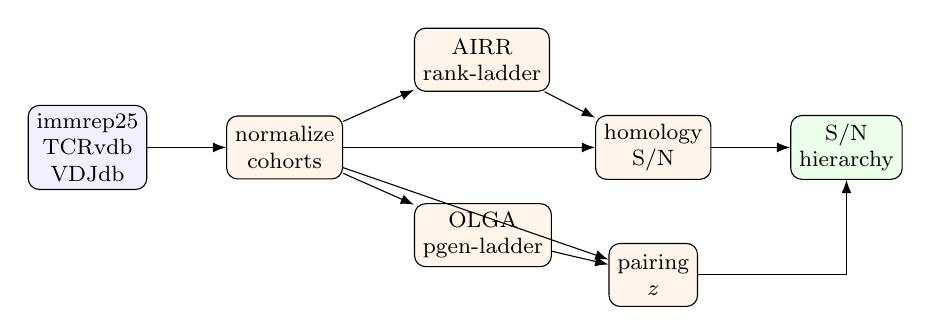
\begin{tikzpicture}[node distance=6mm and 10mm,>=Latex,
  box/.style={draw,rounded corners,align=center,font=\footnotesize,inner sep=3pt,minimum height=8mm},
  data/.style={box,fill=blue!6}, proc/.style={box,fill=orange!8}, result/.style={box,fill=green!8}]
\node[data] (imm) {immrep25\\TCRvdb\\VDJdb};
\node[proc,right=of imm] (coh) {normalize\\cohorts};
\node[proc,above right=3mm and 9mm of coh] (airr) {AIRR\\rank-ladder};
\node[proc,below right=3mm and 9mm of coh] (olga) {OLGA\\pgen-ladder};
\node[proc,right=32mm of coh] (hom) {homology\\S/N};
\node[proc,below=8mm of hom] (pair) {pairing\\$z$};
\node[result,right=10mm of hom] (fig) {S/N\\hierarchy};
\draw[->] (imm)--(coh);
\draw[->] (coh)--(airr); \draw[->] (coh)--(olga);
\draw[->] (airr)--(hom); \draw[->] (olga)--(pair);
\draw[->] (coh)--(hom); \draw[->] (coh)--(pair);
\draw[->] (hom)--(fig); \draw[->] (pair.east)-|(fig);
\end{tikzpicture}
\end{center}

\section{Homology test}\label{sec:homology}

\paragraph{Metric.} For a single chain, TCRs are grouped by epitope. Only
equal-length CDR3s can share a Hamming distance, so pairs are counted within
length bins. With $N_e$ TCRs for epitope $e$ in a cohort of $N$,
\[
P_{\text{self}}=\sum_e \binom{N_e}{2},\qquad
P_{\text{nonself}}=\binom{N}{2}-P_{\text{self}},
\]
(over equal-length pairs) and, writing $m_{\le d}$/$l_{\le d}$ for within-/between-epitope
pairs at Hamming $\le d$,
\[
\mathrm{S/N}(d)=\frac{m_{\le d}/P_{\text{self}}}{l_{\le d}/P_{\text{nonself}}}.
\]
The comparison is of \emph{rates}: non-self pairs vastly outnumber self pairs, so
raw counts are not comparable---only after normalising by $P_{\text{self}}$ and
$P_{\text{nonself}}$ does the enrichment appear. $d{=}0$ isolates publicity
(identical CDR3s); $d{=}1$ is the substitution-neighbour convergence signal
exploited by curated specificity databases~\cite{Shugay_2017}; signal $\Rightarrow$ S/N $\gg 1$, noise $\Rightarrow$
S/N $\approx 1$.

\paragraph{Result.} Figure~\ref{fig:hom} places the cohorts on the S/N axis at the
matched design. The ordering is
VDJdb-HQ $>$ TCRvdb-true $\gtrsim$ TCRvdb-false $>$ VDJdb-LQ $\gg$ immrep25 $>$ OLGA.
On TR$\beta$ the verified cohorts reach S/N $=\hqHomB$ (VDJdb-HQ) and $\trueHomB$
(TCRvdb-true), whereas immrep25 positives give only $\immHomB$ and the
$P_{\text{gen}}$-matched OLGA floor is $\olgaHomB$. The same picture holds on
TR$\alpha$ (immrep25 $\immHomA$ vs.\ OLGA $\olgaHomA$).

\begin{figure}[h]\centering
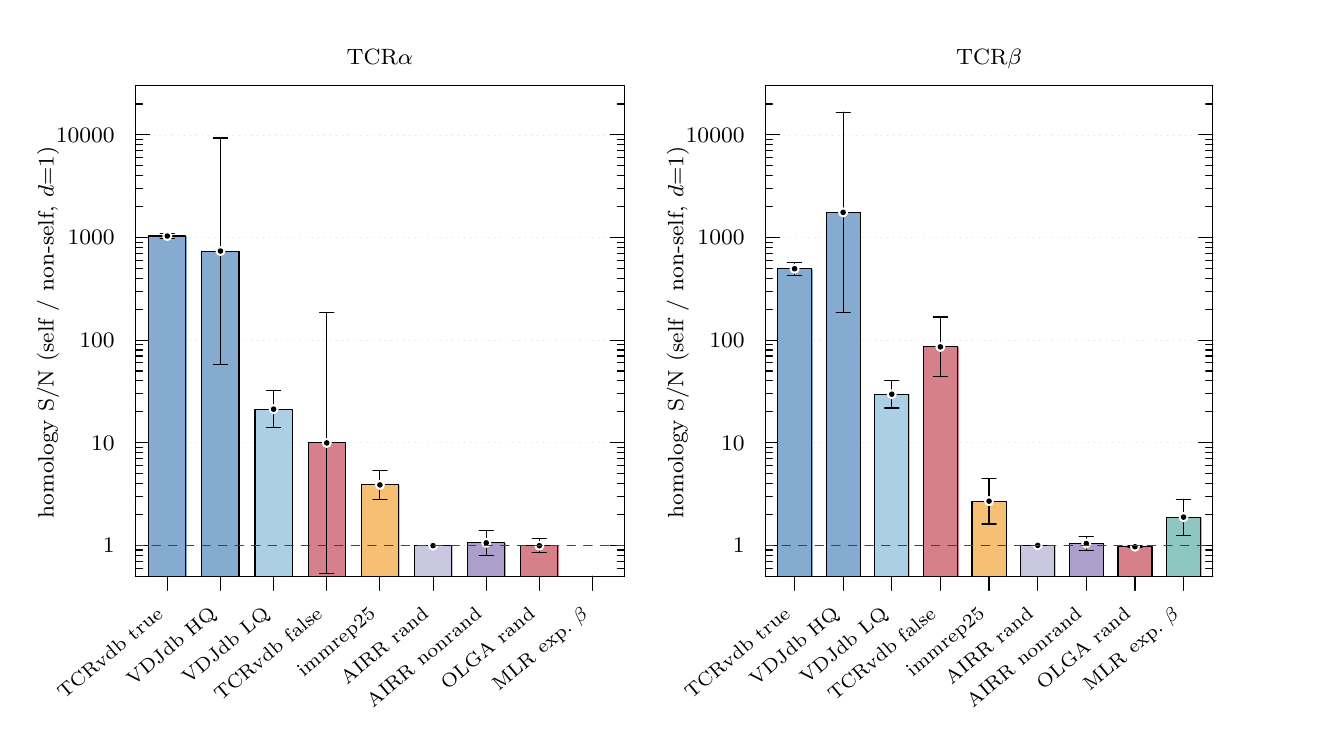
\begin{tikzpicture}[gnuplot]
%% generated with GNUPLOT 6.0p4 (Lua 5.5; terminal rev. Jun 2020, script rev. 120)
%% Sun Jul  5 18:01:10 2026
\tikzset{every node/.append style={font={\fontsize{8.0pt}{9.6pt}\selectfont}}}
\path (0.000,0.000) rectangle (16.000,8.000);
\gpcolor{color=gp lt color border}
\gpsetlinetype{gp lt border}
\gpsetdashtype{gp dt solid}
\gpsetlinewidth{1.00}
\draw[gp path] (1.348,1.033)--(1.438,1.033);
\draw[gp path] (7.558,1.033)--(7.468,1.033);
\draw[gp path] (1.348,1.136)--(1.438,1.136);
\draw[gp path] (7.558,1.136)--(7.468,1.136);
\draw[gp path] (1.348,1.223)--(1.438,1.223);
\draw[gp path] (7.558,1.223)--(7.468,1.223);
\draw[gp path] (1.348,1.299)--(1.438,1.299);
\draw[gp path] (7.558,1.299)--(7.468,1.299);
\draw[gp path] (1.348,1.366)--(1.438,1.366);
\draw[gp path] (7.558,1.366)--(7.468,1.366);
\gpcolor{rgb color={0.867,0.867,0.867}}
\gpsetlinetype{gp lt axes}
\gpsetdashtype{gp dt axes}
\gpsetlinewidth{0.50}
\draw[gp path] (1.348,1.425)--(7.558,1.425);
\gpcolor{color=gp lt color border}
\gpsetlinetype{gp lt border}
\gpsetdashtype{gp dt solid}
\gpsetlinewidth{1.00}
\draw[gp path] (1.348,1.425)--(1.528,1.425);
\draw[gp path] (7.558,1.425)--(7.378,1.425);
\node[gp node right] at (1.201,1.425) {$1$};
\draw[gp path] (1.348,1.818)--(1.438,1.818);
\draw[gp path] (7.558,1.818)--(7.468,1.818);
\draw[gp path] (1.348,2.047)--(1.438,2.047);
\draw[gp path] (7.558,2.047)--(7.468,2.047);
\draw[gp path] (1.348,2.210)--(1.438,2.210);
\draw[gp path] (7.558,2.210)--(7.468,2.210);
\draw[gp path] (1.348,2.336)--(1.438,2.336);
\draw[gp path] (7.558,2.336)--(7.468,2.336);
\draw[gp path] (1.348,2.440)--(1.438,2.440);
\draw[gp path] (7.558,2.440)--(7.468,2.440);
\draw[gp path] (1.348,2.527)--(1.438,2.527);
\draw[gp path] (7.558,2.527)--(7.468,2.527);
\draw[gp path] (1.348,2.602)--(1.438,2.602);
\draw[gp path] (7.558,2.602)--(7.468,2.602);
\draw[gp path] (1.348,2.669)--(1.438,2.669);
\draw[gp path] (7.558,2.669)--(7.468,2.669);
\gpcolor{rgb color={0.867,0.867,0.867}}
\gpsetlinetype{gp lt axes}
\gpsetdashtype{gp dt axes}
\gpsetlinewidth{0.50}
\draw[gp path] (1.348,2.729)--(7.558,2.729);
\gpcolor{color=gp lt color border}
\gpsetlinetype{gp lt border}
\gpsetdashtype{gp dt solid}
\gpsetlinewidth{1.00}
\draw[gp path] (1.348,2.729)--(1.528,2.729);
\draw[gp path] (7.558,2.729)--(7.378,2.729);
\node[gp node right] at (1.201,2.729) {$10$};
\draw[gp path] (1.348,3.121)--(1.438,3.121);
\draw[gp path] (7.558,3.121)--(7.468,3.121);
\draw[gp path] (1.348,3.351)--(1.438,3.351);
\draw[gp path] (7.558,3.351)--(7.468,3.351);
\draw[gp path] (1.348,3.514)--(1.438,3.514);
\draw[gp path] (7.558,3.514)--(7.468,3.514);
\draw[gp path] (1.348,3.640)--(1.438,3.640);
\draw[gp path] (7.558,3.640)--(7.468,3.640);
\draw[gp path] (1.348,3.743)--(1.438,3.743);
\draw[gp path] (7.558,3.743)--(7.468,3.743);
\draw[gp path] (1.348,3.830)--(1.438,3.830);
\draw[gp path] (7.558,3.830)--(7.468,3.830);
\draw[gp path] (1.348,3.906)--(1.438,3.906);
\draw[gp path] (7.558,3.906)--(7.468,3.906);
\draw[gp path] (1.348,3.973)--(1.438,3.973);
\draw[gp path] (7.558,3.973)--(7.468,3.973);
\gpcolor{rgb color={0.867,0.867,0.867}}
\gpsetlinetype{gp lt axes}
\gpsetdashtype{gp dt axes}
\gpsetlinewidth{0.50}
\draw[gp path] (1.348,4.032)--(7.558,4.032);
\gpcolor{color=gp lt color border}
\gpsetlinetype{gp lt border}
\gpsetdashtype{gp dt solid}
\gpsetlinewidth{1.00}
\draw[gp path] (1.348,4.032)--(1.528,4.032);
\draw[gp path] (7.558,4.032)--(7.378,4.032);
\node[gp node right] at (1.201,4.032) {$100$};
\draw[gp path] (1.348,4.425)--(1.438,4.425);
\draw[gp path] (7.558,4.425)--(7.468,4.425);
\draw[gp path] (1.348,4.654)--(1.438,4.654);
\draw[gp path] (7.558,4.654)--(7.468,4.654);
\draw[gp path] (1.348,4.817)--(1.438,4.817);
\draw[gp path] (7.558,4.817)--(7.468,4.817);
\draw[gp path] (1.348,4.943)--(1.438,4.943);
\draw[gp path] (7.558,4.943)--(7.468,4.943);
\draw[gp path] (1.348,5.047)--(1.438,5.047);
\draw[gp path] (7.558,5.047)--(7.468,5.047);
\draw[gp path] (1.348,5.134)--(1.438,5.134);
\draw[gp path] (7.558,5.134)--(7.468,5.134);
\draw[gp path] (1.348,5.209)--(1.438,5.209);
\draw[gp path] (7.558,5.209)--(7.468,5.209);
\draw[gp path] (1.348,5.276)--(1.438,5.276);
\draw[gp path] (7.558,5.276)--(7.468,5.276);
\gpcolor{rgb color={0.867,0.867,0.867}}
\gpsetlinetype{gp lt axes}
\gpsetdashtype{gp dt axes}
\gpsetlinewidth{0.50}
\draw[gp path] (1.348,5.336)--(7.558,5.336);
\gpcolor{color=gp lt color border}
\gpsetlinetype{gp lt border}
\gpsetdashtype{gp dt solid}
\gpsetlinewidth{1.00}
\draw[gp path] (1.348,5.336)--(1.528,5.336);
\draw[gp path] (7.558,5.336)--(7.378,5.336);
\node[gp node right] at (1.201,5.336) {$1000$};
\draw[gp path] (1.348,5.728)--(1.438,5.728);
\draw[gp path] (7.558,5.728)--(7.468,5.728);
\draw[gp path] (1.348,5.958)--(1.438,5.958);
\draw[gp path] (7.558,5.958)--(7.468,5.958);
\draw[gp path] (1.348,6.120)--(1.438,6.120);
\draw[gp path] (7.558,6.120)--(7.468,6.120);
\draw[gp path] (1.348,6.247)--(1.438,6.247);
\draw[gp path] (7.558,6.247)--(7.468,6.247);
\draw[gp path] (1.348,6.350)--(1.438,6.350);
\draw[gp path] (7.558,6.350)--(7.468,6.350);
\draw[gp path] (1.348,6.437)--(1.438,6.437);
\draw[gp path] (7.558,6.437)--(7.468,6.437);
\draw[gp path] (1.348,6.513)--(1.438,6.513);
\draw[gp path] (7.558,6.513)--(7.468,6.513);
\draw[gp path] (1.348,6.579)--(1.438,6.579);
\draw[gp path] (7.558,6.579)--(7.468,6.579);
\gpcolor{rgb color={0.867,0.867,0.867}}
\gpsetlinetype{gp lt axes}
\gpsetdashtype{gp dt axes}
\gpsetlinewidth{0.50}
\draw[gp path] (1.348,6.639)--(7.558,6.639);
\gpcolor{color=gp lt color border}
\gpsetlinetype{gp lt border}
\gpsetdashtype{gp dt solid}
\gpsetlinewidth{1.00}
\draw[gp path] (1.348,6.639)--(1.528,6.639);
\draw[gp path] (7.558,6.639)--(7.378,6.639);
\node[gp node right] at (1.201,6.639) {$10000$};
\draw[gp path] (1.348,7.031)--(1.438,7.031);
\draw[gp path] (7.558,7.031)--(7.468,7.031);
\draw[gp path] (1.348,7.261)--(1.438,7.261);
\draw[gp path] (7.558,7.261)--(7.468,7.261);
\draw[gp path] (1.753,1.033)--(1.753,0.853);
\node[gp node right,rotate=40.0,font={\fontsize{7.0pt}{8.4pt}\selectfont}] at (1.753,0.682) {TCRvdb true};
\draw[gp path] (2.428,1.033)--(2.428,0.853);
\node[gp node right,rotate=40.0,font={\fontsize{7.0pt}{8.4pt}\selectfont}] at (2.428,0.682) {VDJdb HQ};
\draw[gp path] (3.103,1.033)--(3.103,0.853);
\node[gp node right,rotate=40.0,font={\fontsize{7.0pt}{8.4pt}\selectfont}] at (3.103,0.682) {VDJdb LQ};
\draw[gp path] (3.778,1.033)--(3.778,0.853);
\node[gp node right,rotate=40.0,font={\fontsize{7.0pt}{8.4pt}\selectfont}] at (3.778,0.682) {TCRvdb false};
\draw[gp path] (4.453,1.033)--(4.453,0.853);
\node[gp node right,rotate=40.0,font={\fontsize{7.0pt}{8.4pt}\selectfont}] at (4.453,0.682) {immrep25};
\draw[gp path] (5.128,1.033)--(5.128,0.853);
\node[gp node right,rotate=40.0,font={\fontsize{7.0pt}{8.4pt}\selectfont}] at (5.128,0.682) {AIRR rand};
\draw[gp path] (5.803,1.033)--(5.803,0.853);
\node[gp node right,rotate=40.0,font={\fontsize{7.0pt}{8.4pt}\selectfont}] at (5.803,0.682) {AIRR nonrand};
\draw[gp path] (6.478,1.033)--(6.478,0.853);
\node[gp node right,rotate=40.0,font={\fontsize{7.0pt}{8.4pt}\selectfont}] at (6.478,0.682) {OLGA rand};
\draw[gp path] (7.153,1.033)--(7.153,0.853);
\node[gp node right,rotate=40.0,font={\fontsize{7.0pt}{8.4pt}\selectfont}] at (7.153,0.682) {MLR exp.\ $\beta$};
\draw[gp path] (1.348,7.261)--(1.348,1.033)--(7.558,1.033)--(7.558,7.261)--cycle;
\gpfill{rgb color={0.129,0.400,0.675},color=.!55} (1.517,1.033)--(1.990,1.033)--(1.990,5.355)--(1.517,5.355)--cycle;
\draw[gp path] (1.517,1.033)--(1.517,5.354)--(1.989,5.354)--(1.989,1.033)--cycle;
\gpfill{rgb color={0.129,0.400,0.675},color=.!55} (2.192,1.033)--(2.665,1.033)--(2.665,5.164)--(2.192,5.164)--cycle;
\draw[gp path] (2.192,1.033)--(2.192,5.163)--(2.664,5.163)--(2.664,1.033)--cycle;
\gpfill{rgb color={0.404,0.663,0.812},color=.!55} (2.867,1.033)--(3.340,1.033)--(3.340,3.156)--(2.867,3.156)--cycle;
\draw[gp path] (2.867,1.033)--(2.867,3.155)--(3.339,3.155)--(3.339,1.033)--cycle;
\gpfill{rgb color={0.698,0.094,0.169},color=.!55} (3.542,1.033)--(4.015,1.033)--(4.015,2.727)--(3.542,2.727)--cycle;
\draw[gp path] (3.542,1.033)--(3.542,2.726)--(4.014,2.726)--(4.014,1.033)--cycle;
\gpfill{rgb color={0.937,0.541,0.000},color=.!55} (4.217,1.033)--(4.690,1.033)--(4.690,2.194)--(4.217,2.194)--cycle;
\draw[gp path] (4.217,1.033)--(4.217,2.193)--(4.689,2.193)--(4.689,1.033)--cycle;
\gpfill{rgb color={0.620,0.604,0.784},color=.!55} (4.892,1.033)--(5.365,1.033)--(5.365,1.423)--(4.892,1.423)--cycle;
\draw[gp path] (4.892,1.033)--(4.892,1.422)--(5.364,1.422)--(5.364,1.033)--cycle;
\gpfill{rgb color={0.416,0.318,0.639},color=.!55} (5.567,1.033)--(6.040,1.033)--(6.040,1.458)--(5.567,1.458)--cycle;
\draw[gp path] (5.567,1.033)--(5.567,1.457)--(6.039,1.457)--(6.039,1.033)--cycle;
\gpfill{rgb color={0.698,0.094,0.169},color=.!55} (6.242,1.033)--(6.715,1.033)--(6.715,1.422)--(6.242,1.422)--cycle;
\draw[gp path] (6.242,1.033)--(6.242,1.421)--(6.714,1.421)--(6.714,1.033)--cycle;
\gpcolor{rgb color={0.000,0.000,0.000}}
\draw[gp path] (1.753,5.328)--(1.753,5.381);
\draw[gp path] (1.663,5.328)--(1.843,5.328);
\draw[gp path] (1.663,5.381)--(1.843,5.381);
\draw[gp path] (2.428,3.726)--(2.428,6.599);
\draw[gp path] (2.338,3.726)--(2.518,3.726);
\draw[gp path] (2.338,6.599)--(2.518,6.599);
\draw[gp path] (3.103,2.921)--(3.103,3.389);
\draw[gp path] (3.013,2.921)--(3.193,2.921);
\draw[gp path] (3.013,3.389)--(3.193,3.389);
\draw[gp path] (3.778,1.071)--(3.778,4.380);
\draw[gp path] (3.688,1.071)--(3.868,1.071);
\draw[gp path] (3.688,4.380)--(3.868,4.380);
\draw[gp path] (4.453,2.009)--(4.453,2.378);
\draw[gp path] (4.363,2.009)--(4.543,2.009);
\draw[gp path] (4.363,2.378)--(4.543,2.378);
\draw[gp path] (5.128,1.419)--(5.128,1.426);
\draw[gp path] (5.038,1.419)--(5.218,1.419);
\draw[gp path] (5.038,1.426)--(5.218,1.426);
\draw[gp path] (5.803,1.298)--(5.803,1.615);
\draw[gp path] (5.713,1.298)--(5.893,1.298);
\draw[gp path] (5.713,1.615)--(5.893,1.615);
\draw[gp path] (6.478,1.330)--(6.478,1.511);
\draw[gp path] (6.388,1.330)--(6.568,1.330);
\draw[gp path] (6.388,1.511)--(6.568,1.511);
\gpcolor{color=gpbgfillcolor}
\gpsetpointsize{4.00}
\gp3point{gp mark 7}{}{(1.753,5.354)}
\gpcolor{rgb color={0.000,0.000,0.000}}
\gpsetpointsize{2.00}
\gp3point{gp mark 7}{}{(1.753,5.354)}
\gpcolor{color=gpbgfillcolor}
\gpsetpointsize{4.00}
\gp3point{gp mark 7}{}{(2.428,5.163)}
\gpcolor{rgb color={0.000,0.000,0.000}}
\gpsetpointsize{2.00}
\gp3point{gp mark 7}{}{(2.428,5.163)}
\gpcolor{color=gpbgfillcolor}
\gpsetpointsize{4.00}
\gp3point{gp mark 7}{}{(3.103,3.155)}
\gpcolor{rgb color={0.000,0.000,0.000}}
\gpsetpointsize{2.00}
\gp3point{gp mark 7}{}{(3.103,3.155)}
\gpcolor{color=gpbgfillcolor}
\gpsetpointsize{4.00}
\gp3point{gp mark 7}{}{(3.778,2.726)}
\gpcolor{rgb color={0.000,0.000,0.000}}
\gpsetpointsize{2.00}
\gp3point{gp mark 7}{}{(3.778,2.726)}
\gpcolor{color=gpbgfillcolor}
\gpsetpointsize{4.00}
\gp3point{gp mark 7}{}{(4.453,2.193)}
\gpcolor{rgb color={0.000,0.000,0.000}}
\gpsetpointsize{2.00}
\gp3point{gp mark 7}{}{(4.453,2.193)}
\gpcolor{color=gpbgfillcolor}
\gpsetpointsize{4.00}
\gp3point{gp mark 7}{}{(5.128,1.422)}
\gpcolor{rgb color={0.000,0.000,0.000}}
\gpsetpointsize{2.00}
\gp3point{gp mark 7}{}{(5.128,1.422)}
\gpcolor{color=gpbgfillcolor}
\gpsetpointsize{4.00}
\gp3point{gp mark 7}{}{(5.803,1.457)}
\gpcolor{rgb color={0.000,0.000,0.000}}
\gpsetpointsize{2.00}
\gp3point{gp mark 7}{}{(5.803,1.457)}
\gpcolor{color=gpbgfillcolor}
\gpsetpointsize{4.00}
\gp3point{gp mark 7}{}{(6.478,1.421)}
\gpcolor{rgb color={0.000,0.000,0.000}}
\gpsetpointsize{2.00}
\gp3point{gp mark 7}{}{(6.478,1.421)}
\gpcolor{rgb color={0.267,0.267,0.267}}
\gpsetdashtype{gp dt 2}
\draw[gp path] (1.348,1.425)--(1.411,1.425)--(1.473,1.425)--(1.536,1.425)--(1.599,1.425)%
  --(1.662,1.425)--(1.724,1.425)--(1.787,1.425)--(1.850,1.425)--(1.913,1.425)--(1.975,1.425)%
  --(2.038,1.425)--(2.101,1.425)--(2.163,1.425)--(2.226,1.425)--(2.289,1.425)--(2.352,1.425)%
  --(2.414,1.425)--(2.477,1.425)--(2.540,1.425)--(2.603,1.425)--(2.665,1.425)--(2.728,1.425)%
  --(2.791,1.425)--(2.853,1.425)--(2.916,1.425)--(2.979,1.425)--(3.042,1.425)--(3.104,1.425)%
  --(3.167,1.425)--(3.230,1.425)--(3.293,1.425)--(3.355,1.425)--(3.418,1.425)--(3.481,1.425)%
  --(3.543,1.425)--(3.606,1.425)--(3.669,1.425)--(3.732,1.425)--(3.794,1.425)--(3.857,1.425)%
  --(3.920,1.425)--(3.983,1.425)--(4.045,1.425)--(4.108,1.425)--(4.171,1.425)--(4.233,1.425)%
  --(4.296,1.425)--(4.359,1.425)--(4.422,1.425)--(4.484,1.425)--(4.547,1.425)--(4.610,1.425)%
  --(4.673,1.425)--(4.735,1.425)--(4.798,1.425)--(4.861,1.425)--(4.923,1.425)--(4.986,1.425)%
  --(5.049,1.425)--(5.112,1.425)--(5.174,1.425)--(5.237,1.425)--(5.300,1.425)--(5.363,1.425)%
  --(5.425,1.425)--(5.488,1.425)--(5.551,1.425)--(5.613,1.425)--(5.676,1.425)--(5.739,1.425)%
  --(5.802,1.425)--(5.864,1.425)--(5.927,1.425)--(5.990,1.425)--(6.053,1.425)--(6.115,1.425)%
  --(6.178,1.425)--(6.241,1.425)--(6.303,1.425)--(6.366,1.425)--(6.429,1.425)--(6.492,1.425)%
  --(6.554,1.425)--(6.617,1.425)--(6.680,1.425)--(6.743,1.425)--(6.805,1.425)--(6.868,1.425)%
  --(6.931,1.425)--(6.993,1.425)--(7.056,1.425)--(7.119,1.425)--(7.182,1.425)--(7.244,1.425)%
  --(7.307,1.425)--(7.370,1.425)--(7.433,1.425)--(7.495,1.425)--(7.558,1.425);
\gpcolor{color=gp lt color border}
\gpsetdashtype{gp dt solid}
\draw[gp path] (1.348,7.261)--(1.348,1.033)--(7.558,1.033)--(7.558,7.261)--cycle;
\node[gp node center,rotate=-270.0,font={\fontsize{8.0pt}{9.6pt}\selectfont}] at (0.232,4.147) {homology S/N (self / non-self, $d{=}1$)};
\node[gp node center,font={\fontsize{8.0pt}{9.6pt}\selectfont}] at (4.453,7.630) {TCR$\alpha$};
%% coordinates of the plot area
\gpdefrectangularnode{gp plot 1}{\pgfpoint{1.348cm}{1.033cm}}{\pgfpoint{7.558cm}{7.261cm}}
\draw[gp path] (9.348,1.033)--(9.438,1.033);
\draw[gp path] (15.030,1.033)--(14.940,1.033);
\draw[gp path] (9.348,1.136)--(9.438,1.136);
\draw[gp path] (15.030,1.136)--(14.940,1.136);
\draw[gp path] (9.348,1.223)--(9.438,1.223);
\draw[gp path] (15.030,1.223)--(14.940,1.223);
\draw[gp path] (9.348,1.299)--(9.438,1.299);
\draw[gp path] (15.030,1.299)--(14.940,1.299);
\draw[gp path] (9.348,1.366)--(9.438,1.366);
\draw[gp path] (15.030,1.366)--(14.940,1.366);
\gpcolor{rgb color={0.867,0.867,0.867}}
\gpsetlinetype{gp lt axes}
\gpsetdashtype{gp dt axes}
\gpsetlinewidth{0.50}
\draw[gp path] (9.348,1.425)--(15.030,1.425);
\gpcolor{color=gp lt color border}
\gpsetlinetype{gp lt border}
\gpsetdashtype{gp dt solid}
\gpsetlinewidth{1.00}
\draw[gp path] (9.348,1.425)--(9.528,1.425);
\draw[gp path] (15.030,1.425)--(14.850,1.425);
\node[gp node right,font={\fontsize{8.0pt}{9.6pt}\selectfont}] at (9.201,1.425) {$1$};
\draw[gp path] (9.348,1.818)--(9.438,1.818);
\draw[gp path] (15.030,1.818)--(14.940,1.818);
\draw[gp path] (9.348,2.047)--(9.438,2.047);
\draw[gp path] (15.030,2.047)--(14.940,2.047);
\draw[gp path] (9.348,2.210)--(9.438,2.210);
\draw[gp path] (15.030,2.210)--(14.940,2.210);
\draw[gp path] (9.348,2.336)--(9.438,2.336);
\draw[gp path] (15.030,2.336)--(14.940,2.336);
\draw[gp path] (9.348,2.440)--(9.438,2.440);
\draw[gp path] (15.030,2.440)--(14.940,2.440);
\draw[gp path] (9.348,2.527)--(9.438,2.527);
\draw[gp path] (15.030,2.527)--(14.940,2.527);
\draw[gp path] (9.348,2.602)--(9.438,2.602);
\draw[gp path] (15.030,2.602)--(14.940,2.602);
\draw[gp path] (9.348,2.669)--(9.438,2.669);
\draw[gp path] (15.030,2.669)--(14.940,2.669);
\gpcolor{rgb color={0.867,0.867,0.867}}
\gpsetlinetype{gp lt axes}
\gpsetdashtype{gp dt axes}
\gpsetlinewidth{0.50}
\draw[gp path] (9.348,2.729)--(15.030,2.729);
\gpcolor{color=gp lt color border}
\gpsetlinetype{gp lt border}
\gpsetdashtype{gp dt solid}
\gpsetlinewidth{1.00}
\draw[gp path] (9.348,2.729)--(9.528,2.729);
\draw[gp path] (15.030,2.729)--(14.850,2.729);
\node[gp node right,font={\fontsize{8.0pt}{9.6pt}\selectfont}] at (9.201,2.729) {$10$};
\draw[gp path] (9.348,3.121)--(9.438,3.121);
\draw[gp path] (15.030,3.121)--(14.940,3.121);
\draw[gp path] (9.348,3.351)--(9.438,3.351);
\draw[gp path] (15.030,3.351)--(14.940,3.351);
\draw[gp path] (9.348,3.514)--(9.438,3.514);
\draw[gp path] (15.030,3.514)--(14.940,3.514);
\draw[gp path] (9.348,3.640)--(9.438,3.640);
\draw[gp path] (15.030,3.640)--(14.940,3.640);
\draw[gp path] (9.348,3.743)--(9.438,3.743);
\draw[gp path] (15.030,3.743)--(14.940,3.743);
\draw[gp path] (9.348,3.830)--(9.438,3.830);
\draw[gp path] (15.030,3.830)--(14.940,3.830);
\draw[gp path] (9.348,3.906)--(9.438,3.906);
\draw[gp path] (15.030,3.906)--(14.940,3.906);
\draw[gp path] (9.348,3.973)--(9.438,3.973);
\draw[gp path] (15.030,3.973)--(14.940,3.973);
\gpcolor{rgb color={0.867,0.867,0.867}}
\gpsetlinetype{gp lt axes}
\gpsetdashtype{gp dt axes}
\gpsetlinewidth{0.50}
\draw[gp path] (9.348,4.032)--(15.030,4.032);
\gpcolor{color=gp lt color border}
\gpsetlinetype{gp lt border}
\gpsetdashtype{gp dt solid}
\gpsetlinewidth{1.00}
\draw[gp path] (9.348,4.032)--(9.528,4.032);
\draw[gp path] (15.030,4.032)--(14.850,4.032);
\node[gp node right,font={\fontsize{8.0pt}{9.6pt}\selectfont}] at (9.201,4.032) {$100$};
\draw[gp path] (9.348,4.425)--(9.438,4.425);
\draw[gp path] (15.030,4.425)--(14.940,4.425);
\draw[gp path] (9.348,4.654)--(9.438,4.654);
\draw[gp path] (15.030,4.654)--(14.940,4.654);
\draw[gp path] (9.348,4.817)--(9.438,4.817);
\draw[gp path] (15.030,4.817)--(14.940,4.817);
\draw[gp path] (9.348,4.943)--(9.438,4.943);
\draw[gp path] (15.030,4.943)--(14.940,4.943);
\draw[gp path] (9.348,5.047)--(9.438,5.047);
\draw[gp path] (15.030,5.047)--(14.940,5.047);
\draw[gp path] (9.348,5.134)--(9.438,5.134);
\draw[gp path] (15.030,5.134)--(14.940,5.134);
\draw[gp path] (9.348,5.209)--(9.438,5.209);
\draw[gp path] (15.030,5.209)--(14.940,5.209);
\draw[gp path] (9.348,5.276)--(9.438,5.276);
\draw[gp path] (15.030,5.276)--(14.940,5.276);
\gpcolor{rgb color={0.867,0.867,0.867}}
\gpsetlinetype{gp lt axes}
\gpsetdashtype{gp dt axes}
\gpsetlinewidth{0.50}
\draw[gp path] (9.348,5.336)--(15.030,5.336);
\gpcolor{color=gp lt color border}
\gpsetlinetype{gp lt border}
\gpsetdashtype{gp dt solid}
\gpsetlinewidth{1.00}
\draw[gp path] (9.348,5.336)--(9.528,5.336);
\draw[gp path] (15.030,5.336)--(14.850,5.336);
\node[gp node right,font={\fontsize{8.0pt}{9.6pt}\selectfont}] at (9.201,5.336) {$1000$};
\draw[gp path] (9.348,5.728)--(9.438,5.728);
\draw[gp path] (15.030,5.728)--(14.940,5.728);
\draw[gp path] (9.348,5.958)--(9.438,5.958);
\draw[gp path] (15.030,5.958)--(14.940,5.958);
\draw[gp path] (9.348,6.120)--(9.438,6.120);
\draw[gp path] (15.030,6.120)--(14.940,6.120);
\draw[gp path] (9.348,6.247)--(9.438,6.247);
\draw[gp path] (15.030,6.247)--(14.940,6.247);
\draw[gp path] (9.348,6.350)--(9.438,6.350);
\draw[gp path] (15.030,6.350)--(14.940,6.350);
\draw[gp path] (9.348,6.437)--(9.438,6.437);
\draw[gp path] (15.030,6.437)--(14.940,6.437);
\draw[gp path] (9.348,6.513)--(9.438,6.513);
\draw[gp path] (15.030,6.513)--(14.940,6.513);
\draw[gp path] (9.348,6.579)--(9.438,6.579);
\draw[gp path] (15.030,6.579)--(14.940,6.579);
\gpcolor{rgb color={0.867,0.867,0.867}}
\gpsetlinetype{gp lt axes}
\gpsetdashtype{gp dt axes}
\gpsetlinewidth{0.50}
\draw[gp path] (9.348,6.639)--(15.030,6.639);
\gpcolor{color=gp lt color border}
\gpsetlinetype{gp lt border}
\gpsetdashtype{gp dt solid}
\gpsetlinewidth{1.00}
\draw[gp path] (9.348,6.639)--(9.528,6.639);
\draw[gp path] (15.030,6.639)--(14.850,6.639);
\node[gp node right,font={\fontsize{8.0pt}{9.6pt}\selectfont}] at (9.201,6.639) {$10000$};
\draw[gp path] (9.348,7.031)--(9.438,7.031);
\draw[gp path] (15.030,7.031)--(14.940,7.031);
\draw[gp path] (9.348,7.261)--(9.438,7.261);
\draw[gp path] (15.030,7.261)--(14.940,7.261);
\draw[gp path] (9.719,1.033)--(9.719,0.853);
\node[gp node right,rotate=40.0,font={\fontsize{7.0pt}{8.4pt}\selectfont}] at (9.719,0.682) {TCRvdb true};
\draw[gp path] (10.336,1.033)--(10.336,0.853);
\node[gp node right,rotate=40.0,font={\fontsize{7.0pt}{8.4pt}\selectfont}] at (10.336,0.682) {VDJdb HQ};
\draw[gp path] (10.954,1.033)--(10.954,0.853);
\node[gp node right,rotate=40.0,font={\fontsize{7.0pt}{8.4pt}\selectfont}] at (10.954,0.682) {VDJdb LQ};
\draw[gp path] (11.571,1.033)--(11.571,0.853);
\node[gp node right,rotate=40.0,font={\fontsize{7.0pt}{8.4pt}\selectfont}] at (11.571,0.682) {TCRvdb false};
\draw[gp path] (12.189,1.033)--(12.189,0.853);
\node[gp node right,rotate=40.0,font={\fontsize{7.0pt}{8.4pt}\selectfont}] at (12.189,0.682) {immrep25};
\draw[gp path] (12.807,1.033)--(12.807,0.853);
\node[gp node right,rotate=40.0,font={\fontsize{7.0pt}{8.4pt}\selectfont}] at (12.807,0.682) {AIRR rand};
\draw[gp path] (13.424,1.033)--(13.424,0.853);
\node[gp node right,rotate=40.0,font={\fontsize{7.0pt}{8.4pt}\selectfont}] at (13.424,0.682) {AIRR nonrand};
\draw[gp path] (14.042,1.033)--(14.042,0.853);
\node[gp node right,rotate=40.0,font={\fontsize{7.0pt}{8.4pt}\selectfont}] at (14.042,0.682) {OLGA rand};
\draw[gp path] (14.659,1.033)--(14.659,0.853);
\node[gp node right,rotate=40.0,font={\fontsize{7.0pt}{8.4pt}\selectfont}] at (14.659,0.682) {MLR exp.\ $\beta$};
\draw[gp path] (9.348,7.261)--(9.348,1.033)--(15.030,1.033)--(15.030,7.261)--cycle;
\gpfill{rgb color={0.129,0.400,0.675},color=.!55} (9.502,1.033)--(9.936,1.033)--(9.936,4.939)--(9.502,4.939)--cycle;
\draw[gp path] (9.502,1.033)--(9.502,4.938)--(9.935,4.938)--(9.935,1.033)--cycle;
\gpfill{rgb color={0.129,0.400,0.675},color=.!55} (10.120,1.033)--(10.553,1.033)--(10.553,5.655)--(10.120,5.655)--cycle;
\draw[gp path] (10.120,1.033)--(10.120,5.654)--(10.552,5.654)--(10.552,1.033)--cycle;
\gpfill{rgb color={0.404,0.663,0.812},color=.!55} (10.738,1.033)--(11.171,1.033)--(11.171,3.346)--(10.738,3.346)--cycle;
\draw[gp path] (10.738,1.033)--(10.738,3.345)--(11.170,3.345)--(11.170,1.033)--cycle;
\gpfill{rgb color={0.698,0.094,0.169},color=.!55} (11.355,1.033)--(11.789,1.033)--(11.789,3.947)--(11.355,3.947)--cycle;
\draw[gp path] (11.355,1.033)--(11.355,3.946)--(11.788,3.946)--(11.788,1.033)--cycle;
\gpfill{rgb color={0.937,0.541,0.000},color=.!55} (11.973,1.033)--(12.406,1.033)--(12.406,1.988)--(11.973,1.988)--cycle;
\draw[gp path] (11.973,1.033)--(11.973,1.987)--(12.405,1.987)--(12.405,1.033)--cycle;
\gpfill{rgb color={0.620,0.604,0.784},color=.!55} (12.590,1.033)--(13.024,1.033)--(13.024,1.426)--(12.590,1.426)--cycle;
\draw[gp path] (12.590,1.033)--(12.590,1.425)--(13.023,1.425)--(13.023,1.033)--cycle;
\gpfill{rgb color={0.416,0.318,0.639},color=.!55} (13.208,1.033)--(13.641,1.033)--(13.641,1.450)--(13.208,1.450)--cycle;
\draw[gp path] (13.208,1.033)--(13.208,1.449)--(13.640,1.449)--(13.640,1.033)--cycle;
\gpfill{rgb color={0.698,0.094,0.169},color=.!55} (13.826,1.033)--(14.259,1.033)--(14.259,1.409)--(13.826,1.409)--cycle;
\draw[gp path] (13.826,1.033)--(13.826,1.408)--(14.258,1.408)--(14.258,1.033)--cycle;
\gpfill{rgb color={0.208,0.592,0.561},color=.!55} (14.443,1.033)--(14.877,1.033)--(14.877,1.785)--(14.443,1.785)--cycle;
\draw[gp path] (14.443,1.033)--(14.443,1.784)--(14.876,1.784)--(14.876,1.033)--cycle;
\gpcolor{rgb color={0.000,0.000,0.000}}
\draw[gp path] (9.719,4.858)--(9.719,5.019);
\draw[gp path] (9.629,4.858)--(9.809,4.858);
\draw[gp path] (9.629,5.019)--(9.809,5.019);
\draw[gp path] (10.336,4.383)--(10.336,6.926);
\draw[gp path] (10.246,4.383)--(10.426,4.383);
\draw[gp path] (10.246,6.926)--(10.426,6.926);
\draw[gp path] (10.954,3.170)--(10.954,3.519);
\draw[gp path] (10.864,3.170)--(11.044,3.170);
\draw[gp path] (10.864,3.519)--(11.044,3.519);
\draw[gp path] (11.571,3.566)--(11.571,4.326);
\draw[gp path] (11.481,3.566)--(11.661,3.566);
\draw[gp path] (11.481,4.326)--(11.661,4.326);
\draw[gp path] (12.189,1.697)--(12.189,2.276);
\draw[gp path] (12.099,1.697)--(12.279,1.697);
\draw[gp path] (12.099,2.276)--(12.279,2.276);
\draw[gp path] (12.717,1.425)--(12.897,1.425);
\draw[gp path] (12.717,1.425)--(12.897,1.425);
\draw[gp path] (13.424,1.362)--(13.424,1.535);
\draw[gp path] (13.334,1.362)--(13.514,1.362);
\draw[gp path] (13.334,1.535)--(13.514,1.535);
\draw[gp path] (14.042,1.399)--(14.042,1.417);
\draw[gp path] (13.952,1.399)--(14.132,1.399);
\draw[gp path] (13.952,1.417)--(14.132,1.417);
\draw[gp path] (14.659,1.556)--(14.659,2.011);
\draw[gp path] (14.569,1.556)--(14.749,1.556);
\draw[gp path] (14.569,2.011)--(14.749,2.011);
\gpcolor{color=gpbgfillcolor}
\gpsetpointsize{4.00}
\gp3point{gp mark 7}{}{(9.719,4.938)}
\gpcolor{rgb color={0.000,0.000,0.000}}
\gpsetpointsize{2.00}
\gp3point{gp mark 7}{}{(9.719,4.938)}
\gpcolor{color=gpbgfillcolor}
\gpsetpointsize{4.00}
\gp3point{gp mark 7}{}{(10.336,5.654)}
\gpcolor{rgb color={0.000,0.000,0.000}}
\gpsetpointsize{2.00}
\gp3point{gp mark 7}{}{(10.336,5.654)}
\gpcolor{color=gpbgfillcolor}
\gpsetpointsize{4.00}
\gp3point{gp mark 7}{}{(10.954,3.345)}
\gpcolor{rgb color={0.000,0.000,0.000}}
\gpsetpointsize{2.00}
\gp3point{gp mark 7}{}{(10.954,3.345)}
\gpcolor{color=gpbgfillcolor}
\gpsetpointsize{4.00}
\gp3point{gp mark 7}{}{(11.571,3.946)}
\gpcolor{rgb color={0.000,0.000,0.000}}
\gpsetpointsize{2.00}
\gp3point{gp mark 7}{}{(11.571,3.946)}
\gpcolor{color=gpbgfillcolor}
\gpsetpointsize{4.00}
\gp3point{gp mark 7}{}{(12.189,1.987)}
\gpcolor{rgb color={0.000,0.000,0.000}}
\gpsetpointsize{2.00}
\gp3point{gp mark 7}{}{(12.189,1.987)}
\gpcolor{color=gpbgfillcolor}
\gpsetpointsize{4.00}
\gp3point{gp mark 7}{}{(12.807,1.425)}
\gpcolor{rgb color={0.000,0.000,0.000}}
\gpsetpointsize{2.00}
\gp3point{gp mark 7}{}{(12.807,1.425)}
\gpcolor{color=gpbgfillcolor}
\gpsetpointsize{4.00}
\gp3point{gp mark 7}{}{(13.424,1.449)}
\gpcolor{rgb color={0.000,0.000,0.000}}
\gpsetpointsize{2.00}
\gp3point{gp mark 7}{}{(13.424,1.449)}
\gpcolor{color=gpbgfillcolor}
\gpsetpointsize{4.00}
\gp3point{gp mark 7}{}{(14.042,1.408)}
\gpcolor{rgb color={0.000,0.000,0.000}}
\gpsetpointsize{2.00}
\gp3point{gp mark 7}{}{(14.042,1.408)}
\gpcolor{color=gpbgfillcolor}
\gpsetpointsize{4.00}
\gp3point{gp mark 7}{}{(14.659,1.784)}
\gpcolor{rgb color={0.000,0.000,0.000}}
\gpsetpointsize{2.00}
\gp3point{gp mark 7}{}{(14.659,1.784)}
\gpcolor{rgb color={0.267,0.267,0.267}}
\gpsetdashtype{gp dt 2}
\draw[gp path] (9.348,1.425)--(9.405,1.425)--(9.463,1.425)--(9.520,1.425)--(9.578,1.425)%
  --(9.635,1.425)--(9.692,1.425)--(9.750,1.425)--(9.807,1.425)--(9.865,1.425)--(9.922,1.425)%
  --(9.979,1.425)--(10.037,1.425)--(10.094,1.425)--(10.152,1.425)--(10.209,1.425)--(10.266,1.425)%
  --(10.324,1.425)--(10.381,1.425)--(10.438,1.425)--(10.496,1.425)--(10.553,1.425)--(10.611,1.425)%
  --(10.668,1.425)--(10.725,1.425)--(10.783,1.425)--(10.840,1.425)--(10.898,1.425)--(10.955,1.425)%
  --(11.012,1.425)--(11.070,1.425)--(11.127,1.425)--(11.185,1.425)--(11.242,1.425)--(11.299,1.425)%
  --(11.357,1.425)--(11.414,1.425)--(11.472,1.425)--(11.529,1.425)--(11.586,1.425)--(11.644,1.425)%
  --(11.701,1.425)--(11.759,1.425)--(11.816,1.425)--(11.873,1.425)--(11.931,1.425)--(11.988,1.425)%
  --(12.046,1.425)--(12.103,1.425)--(12.160,1.425)--(12.218,1.425)--(12.275,1.425)--(12.332,1.425)%
  --(12.390,1.425)--(12.447,1.425)--(12.505,1.425)--(12.562,1.425)--(12.619,1.425)--(12.677,1.425)%
  --(12.734,1.425)--(12.792,1.425)--(12.849,1.425)--(12.906,1.425)--(12.964,1.425)--(13.021,1.425)%
  --(13.079,1.425)--(13.136,1.425)--(13.193,1.425)--(13.251,1.425)--(13.308,1.425)--(13.366,1.425)%
  --(13.423,1.425)--(13.480,1.425)--(13.538,1.425)--(13.595,1.425)--(13.653,1.425)--(13.710,1.425)%
  --(13.767,1.425)--(13.825,1.425)--(13.882,1.425)--(13.940,1.425)--(13.997,1.425)--(14.054,1.425)%
  --(14.112,1.425)--(14.169,1.425)--(14.226,1.425)--(14.284,1.425)--(14.341,1.425)--(14.399,1.425)%
  --(14.456,1.425)--(14.513,1.425)--(14.571,1.425)--(14.628,1.425)--(14.686,1.425)--(14.743,1.425)%
  --(14.800,1.425)--(14.858,1.425)--(14.915,1.425)--(14.973,1.425)--(15.030,1.425);
\gpcolor{color=gp lt color border}
\gpsetdashtype{gp dt solid}
\draw[gp path] (9.348,7.261)--(9.348,1.033)--(15.030,1.033)--(15.030,7.261)--cycle;
\node[gp node center,rotate=-270.0,font={\fontsize{8.0pt}{9.6pt}\selectfont}] at (8.232,4.147) {homology S/N (self / non-self, $d{=}1$)};
\node[gp node center,font={\fontsize{8.0pt}{9.6pt}\selectfont}] at (12.189,7.630) {TCR$\beta$};
%% coordinates of the plot area
\gpdefrectangularnode{gp plot 2}{\pgfpoint{9.348cm}{1.033cm}}{\pgfpoint{15.030cm}{7.261cm}}
\end{tikzpicture}
%% gnuplot variables

\caption{Homology S/N ($d{=}1$) per cohort, TR$\alpha$ and TR$\beta$, matched
design ($E{=}2$, $K{=}30$, 200 bootstraps; bars = median, whiskers = 95\% CI).
The whiskers are bootstrap confidence intervals over resampled epitopes \emph{and}
TCRs, so their width mainly reflects between-epitope variation (each bootstrap draws
$E{=}2$ epitopes; per-epitope $n{=}50$ for immrep25). Dashed line: noise floor
S/N${=}1$. immrep25 positives sit just above the OLGA random floor and far below
every quality cohort.}
\label{fig:hom}
\end{figure}

\paragraph{By-epitope breakdown.} To show what drives those intervals,
Fig.~\ref{fig:bee} plots the within-epitope neighbour rate for every epitope with
$n\ge 50$ (one point per epitope); the vertical gap to each cohort's non-self rate
(red bar) is the S/N. immrep25's swarm hugs its non-self line, whereas the verified
cohorts sit orders of magnitude above. Table~\ref{tab:epi} lists all 20 immrep25
epitopes: in total they contribute only $\immWithinB$ (TR$\beta$) / $\immWithinA$
(TR$\alpha$) within-epitope Hamming-$1$ neighbours --- versus $\olgaWithinB$ /
$\olgaWithinA$ for the $P_{\text{gen}}$-matched OLGA control and tens of thousands
for the VDJdb cohorts --- and even that handful is concentrated in a few epitopes
(e.g.\ YLFNADIWI) and is entirely public (\S\ref{sec:publicity}).

\begin{figure}[h]\centering
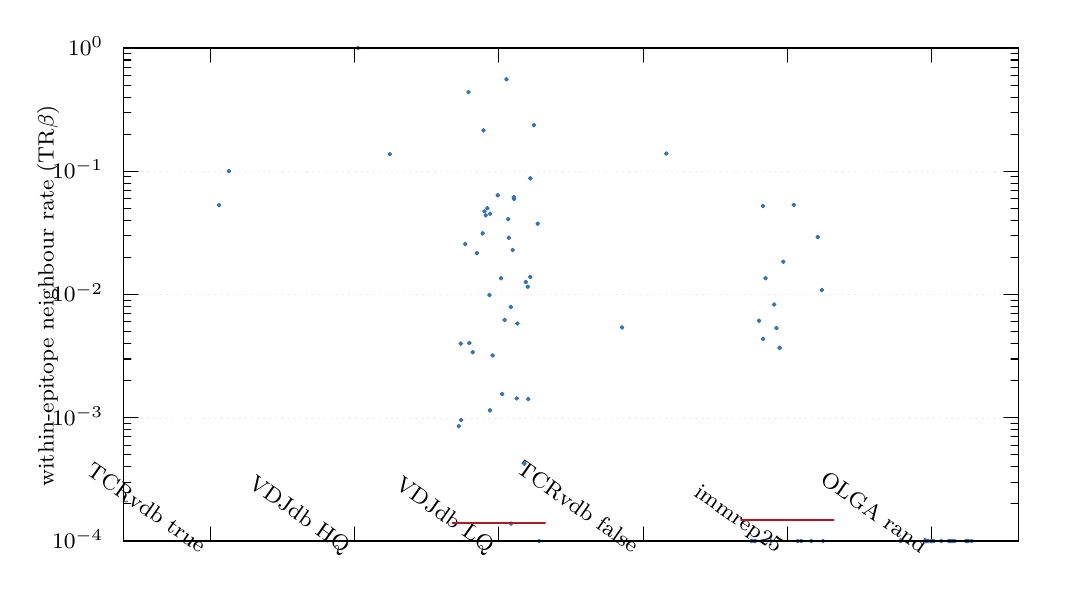
\begin{tikzpicture}[gnuplot]
%% generated with GNUPLOT 6.0p4 (Lua 5.5; terminal rev. Jun 2020, script rev. 120)
%% Fri Jul  3 23:53:18 2026
\tikzset{every node/.append style={font={\fontsize{8.0pt}{9.6pt}\selectfont}}}
\path (0.000,0.000) rectangle (13.000,7.000);
\gpcolor{rgb color={0.867,0.867,0.867}}
\gpsetlinetype{gp lt axes}
\gpsetdashtype{gp dt axes}
\gpsetlinewidth{0.50}
\draw[gp path] (1.201,0.492)--(12.558,0.492);
\gpcolor{color=gp lt color border}
\gpsetlinetype{gp lt border}
\gpsetdashtype{gp dt solid}
\gpsetlinewidth{1.00}
\draw[gp path] (1.201,0.492)--(1.381,0.492);
\draw[gp path] (12.558,0.492)--(12.378,0.492);
\node[gp node right] at (1.054,0.492) {$10^{-4}$};
\draw[gp path] (1.201,0.963)--(1.291,0.963);
\draw[gp path] (12.558,0.963)--(12.468,0.963);
\draw[gp path] (1.201,1.239)--(1.291,1.239);
\draw[gp path] (12.558,1.239)--(12.468,1.239);
\draw[gp path] (1.201,1.434)--(1.291,1.434);
\draw[gp path] (12.558,1.434)--(12.468,1.434);
\draw[gp path] (1.201,1.586)--(1.291,1.586);
\draw[gp path] (12.558,1.586)--(12.468,1.586);
\draw[gp path] (1.201,1.710)--(1.291,1.710);
\draw[gp path] (12.558,1.710)--(12.468,1.710);
\draw[gp path] (1.201,1.815)--(1.291,1.815);
\draw[gp path] (12.558,1.815)--(12.468,1.815);
\draw[gp path] (1.201,1.906)--(1.291,1.906);
\draw[gp path] (12.558,1.906)--(12.468,1.906);
\draw[gp path] (1.201,1.986)--(1.291,1.986);
\draw[gp path] (12.558,1.986)--(12.468,1.986);
\gpcolor{rgb color={0.867,0.867,0.867}}
\gpsetlinetype{gp lt axes}
\gpsetdashtype{gp dt axes}
\gpsetlinewidth{0.50}
\draw[gp path] (1.201,2.057)--(12.558,2.057);
\gpcolor{color=gp lt color border}
\gpsetlinetype{gp lt border}
\gpsetdashtype{gp dt solid}
\gpsetlinewidth{1.00}
\draw[gp path] (1.201,2.057)--(1.381,2.057);
\draw[gp path] (12.558,2.057)--(12.378,2.057);
\node[gp node right] at (1.054,2.057) {$10^{-3}$};
\draw[gp path] (1.201,2.528)--(1.291,2.528);
\draw[gp path] (12.558,2.528)--(12.468,2.528);
\draw[gp path] (1.201,2.804)--(1.291,2.804);
\draw[gp path] (12.558,2.804)--(12.468,2.804);
\draw[gp path] (1.201,3.000)--(1.291,3.000);
\draw[gp path] (12.558,3.000)--(12.468,3.000);
\draw[gp path] (1.201,3.151)--(1.291,3.151);
\draw[gp path] (12.558,3.151)--(12.468,3.151);
\draw[gp path] (1.201,3.275)--(1.291,3.275);
\draw[gp path] (12.558,3.275)--(12.468,3.275);
\draw[gp path] (1.201,3.380)--(1.291,3.380);
\draw[gp path] (12.558,3.380)--(12.468,3.380);
\draw[gp path] (1.201,3.471)--(1.291,3.471);
\draw[gp path] (12.558,3.471)--(12.468,3.471);
\draw[gp path] (1.201,3.551)--(1.291,3.551);
\draw[gp path] (12.558,3.551)--(12.468,3.551);
\gpcolor{rgb color={0.867,0.867,0.867}}
\gpsetlinetype{gp lt axes}
\gpsetdashtype{gp dt axes}
\gpsetlinewidth{0.50}
\draw[gp path] (1.201,3.623)--(12.558,3.623);
\gpcolor{color=gp lt color border}
\gpsetlinetype{gp lt border}
\gpsetdashtype{gp dt solid}
\gpsetlinewidth{1.00}
\draw[gp path] (1.201,3.623)--(1.381,3.623);
\draw[gp path] (12.558,3.623)--(12.378,3.623);
\node[gp node right] at (1.054,3.623) {$10^{-2}$};
\draw[gp path] (1.201,4.094)--(1.291,4.094);
\draw[gp path] (12.558,4.094)--(12.468,4.094);
\draw[gp path] (1.201,4.369)--(1.291,4.369);
\draw[gp path] (12.558,4.369)--(12.468,4.369);
\draw[gp path] (1.201,4.565)--(1.291,4.565);
\draw[gp path] (12.558,4.565)--(12.468,4.565);
\draw[gp path] (1.201,4.717)--(1.291,4.717);
\draw[gp path] (12.558,4.717)--(12.468,4.717);
\draw[gp path] (1.201,4.841)--(1.291,4.841);
\draw[gp path] (12.558,4.841)--(12.468,4.841);
\draw[gp path] (1.201,4.945)--(1.291,4.945);
\draw[gp path] (12.558,4.945)--(12.468,4.945);
\draw[gp path] (1.201,5.036)--(1.291,5.036);
\draw[gp path] (12.558,5.036)--(12.468,5.036);
\draw[gp path] (1.201,5.116)--(1.291,5.116);
\draw[gp path] (12.558,5.116)--(12.468,5.116);
\gpcolor{rgb color={0.867,0.867,0.867}}
\gpsetlinetype{gp lt axes}
\gpsetdashtype{gp dt axes}
\gpsetlinewidth{0.50}
\draw[gp path] (1.201,5.188)--(12.558,5.188);
\gpcolor{color=gp lt color border}
\gpsetlinetype{gp lt border}
\gpsetdashtype{gp dt solid}
\gpsetlinewidth{1.00}
\draw[gp path] (1.201,5.188)--(1.381,5.188);
\draw[gp path] (12.558,5.188)--(12.378,5.188);
\node[gp node right] at (1.054,5.188) {$10^{-1}$};
\draw[gp path] (1.201,5.659)--(1.291,5.659);
\draw[gp path] (12.558,5.659)--(12.468,5.659);
\draw[gp path] (1.201,5.935)--(1.291,5.935);
\draw[gp path] (12.558,5.935)--(12.468,5.935);
\draw[gp path] (1.201,6.130)--(1.291,6.130);
\draw[gp path] (12.558,6.130)--(12.468,6.130);
\draw[gp path] (1.201,6.282)--(1.291,6.282);
\draw[gp path] (12.558,6.282)--(12.468,6.282);
\draw[gp path] (1.201,6.406)--(1.291,6.406);
\draw[gp path] (12.558,6.406)--(12.468,6.406);
\draw[gp path] (1.201,6.511)--(1.291,6.511);
\draw[gp path] (12.558,6.511)--(12.468,6.511);
\draw[gp path] (1.201,6.601)--(1.291,6.601);
\draw[gp path] (12.558,6.601)--(12.468,6.601);
\draw[gp path] (1.201,6.681)--(1.291,6.681);
\draw[gp path] (12.558,6.681)--(12.468,6.681);
\gpcolor{rgb color={0.867,0.867,0.867}}
\gpsetlinetype{gp lt axes}
\gpsetdashtype{gp dt axes}
\gpsetlinewidth{0.50}
\draw[gp path] (1.201,6.753)--(12.558,6.753);
\gpcolor{color=gp lt color border}
\gpsetlinetype{gp lt border}
\gpsetdashtype{gp dt solid}
\gpsetlinewidth{1.00}
\draw[gp path] (1.201,6.753)--(1.381,6.753);
\draw[gp path] (12.558,6.753)--(12.378,6.753);
\node[gp node right] at (1.054,6.753) {$10^{0}$};
\draw[gp path] (2.300,0.492)--(2.300,0.672);
\draw[gp path] (2.300,6.753)--(2.300,6.573);
\node[gp node right,rotate=-35.0] at (2.300,0.345) {TCRvdb true};
\draw[gp path] (4.132,0.492)--(4.132,0.672);
\draw[gp path] (4.132,6.753)--(4.132,6.573);
\node[gp node right,rotate=-35.0] at (4.132,0.345) {VDJdb HQ};
\draw[gp path] (5.964,0.492)--(5.964,0.672);
\draw[gp path] (5.964,6.753)--(5.964,6.573);
\node[gp node right,rotate=-35.0] at (5.964,0.345) {VDJdb LQ};
\draw[gp path] (7.795,0.492)--(7.795,0.672);
\draw[gp path] (7.795,6.753)--(7.795,6.573);
\node[gp node right,rotate=-35.0] at (7.795,0.345) {TCRvdb false};
\draw[gp path] (9.627,0.492)--(9.627,0.672);
\draw[gp path] (9.627,6.753)--(9.627,6.573);
\node[gp node right,rotate=-35.0] at (9.627,0.345) {immrep25};
\draw[gp path] (11.459,0.492)--(11.459,0.672);
\draw[gp path] (11.459,6.753)--(11.459,6.573);
\node[gp node right,rotate=-35.0] at (11.459,0.345) {OLGA rand};
\draw[gp path] (1.201,6.753)--(1.201,0.492)--(12.558,0.492)--(12.558,6.753)--cycle;
\gpcolor{rgb color={0.208,0.451,0.725}}
\gpsetpointsize{1.60}
\gp3point{gp mark 7}{}{(2.409,4.758)}
\gp3point{gp mark 7}{}{(2.535,5.189)}
\gp3point{gp mark 7}{}{(4.177,6.753)}
\gp3point{gp mark 7}{}{(4.578,5.406)}
\gp3point{gp mark 7}{}{(6.288,1.475)}
\gp3point{gp mark 7}{}{(5.454,1.951)}
\gp3point{gp mark 7}{}{(6.330,3.721)}
\gp3point{gp mark 7}{}{(5.485,2.029)}
\gp3point{gp mark 7}{}{(6.199,3.254)}
\gp3point{gp mark 7}{}{(5.631,2.890)}
\gp3point{gp mark 7}{}{(6.336,2.294)}
\gp3point{gp mark 7}{}{(6.006,2.358)}
\gp3point{gp mark 7}{}{(5.758,4.399)}
\gp3point{gp mark 7}{}{(5.884,2.849)}
\gp3point{gp mark 7}{}{(5.480,2.999)}
\gp3point{gp mark 7}{}{(5.578,6.193)}
\gp3point{gp mark 7}{}{(6.139,4.188)}
\gp3point{gp mark 7}{}{(6.115,3.465)}
\gp3point{gp mark 7}{}{(6.082,4.579)}
\gp3point{gp mark 7}{}{(5.844,3.616)}
\gp3point{gp mark 7}{}{(6.474,0.492)}
\gp3point{gp mark 7}{}{(6.457,4.522)}
\gp3point{gp mark 7}{}{(6.154,4.859)}
\gp3point{gp mark 7}{}{(6.118,0.713)}
\gp3point{gp mark 7}{}{(6.157,4.836)}
\gp3point{gp mark 7}{}{(5.850,2.151)}
\gp3point{gp mark 7}{}{(5.589,3.006)}
\gp3point{gp mark 7}{}{(6.191,2.303)}
\gp3point{gp mark 7}{}{(5.990,3.828)}
\gp3point{gp mark 7}{}{(5.769,5.707)}
\gp3point{gp mark 7}{}{(5.949,4.883)}
\gp3point{gp mark 7}{}{(6.363,3.846)}
\gp3point{gp mark 7}{}{(6.409,5.773)}
\gp3point{gp mark 7}{}{(5.818,4.718)}
\gp3point{gp mark 7}{}{(6.037,3.299)}
\gp3point{gp mark 7}{}{(5.781,4.679)}
\gp3point{gp mark 7}{}{(6.060,6.356)}
\gp3point{gp mark 7}{}{(5.797,4.628)}
\gp3point{gp mark 7}{}{(5.852,4.648)}
\gp3point{gp mark 7}{}{(6.364,5.097)}
\gp3point{gp mark 7}{}{(5.684,4.148)}
\gp3point{gp mark 7}{}{(6.090,4.343)}
\gp3point{gp mark 7}{}{(5.537,4.263)}
\gp3point{gp mark 7}{}{(6.305,3.781)}
\gp3point{gp mark 7}{}{(8.090,5.413)}
\gp3point{gp mark 7}{}{(7.528,3.204)}
\gp3point{gp mark 7}{}{(10.013,4.352)}
\gp3point{gp mark 7}{}{(9.174,0.492)}
\gp3point{gp mark 7}{}{(9.459,3.496)}
\gp3point{gp mark 7}{}{(9.268,3.290)}
\gp3point{gp mark 7}{}{(9.576,4.039)}
\gp3point{gp mark 7}{}{(9.931,0.492)}
\gp3point{gp mark 7}{}{(9.351,3.830)}
\gp3point{gp mark 7}{}{(9.168,0.492)}
\gp3point{gp mark 7}{}{(9.529,2.945)}
\gp3point{gp mark 7}{}{(9.318,4.746)}
\gp3point{gp mark 7}{}{(9.207,0.492)}
\gp3point{gp mark 7}{}{(9.710,4.760)}
\gp3point{gp mark 7}{}{(9.421,0.492)}
\gp3point{gp mark 7}{}{(9.804,0.492)}
\gp3point{gp mark 7}{}{(9.319,3.059)}
\gp3point{gp mark 7}{}{(10.081,0.492)}
\gp3point{gp mark 7}{}{(9.489,3.197)}
\gp3point{gp mark 7}{}{(9.222,0.492)}
\gp3point{gp mark 7}{}{(9.760,0.492)}
\gp3point{gp mark 7}{}{(10.065,3.679)}
\gp3point{gp mark 7}{}{(11.398,0.492)}
\gp3point{gp mark 7}{}{(11.925,0.492)}
\gp3point{gp mark 7}{}{(11.459,0.492)}
\gp3point{gp mark 7}{}{(11.382,0.492)}
\gp3point{gp mark 7}{}{(11.582,0.492)}
\gp3point{gp mark 7}{}{(11.967,0.492)}
\gp3point{gp mark 7}{}{(11.919,0.492)}
\gp3point{gp mark 7}{}{(11.418,0.492)}
\gp3point{gp mark 7}{}{(11.723,0.492)}
\gp3point{gp mark 7}{}{(11.456,0.492)}
\gp3point{gp mark 7}{}{(11.489,0.492)}
\gp3point{gp mark 7}{}{(11.752,0.492)}
\gp3point{gp mark 7}{}{(11.371,0.492)}
\gp3point{gp mark 7}{}{(11.699,0.492)}
\gp3point{gp mark 7}{}{(11.676,0.492)}
\gp3point{gp mark 7}{}{(11.902,0.492)}
\gp3point{gp mark 7}{}{(11.064,0.492)}
\gp3point{gp mark 7}{}{(11.694,0.492)}
\gp3point{gp mark 7}{}{(11.897,0.492)}
\gpcolor{rgb color={0.698,0.094,0.169}}
\gpsetlinewidth{2.00}
\draw[gp path](1.714,0.492)--(2.886,0.492);
\draw[gp path](3.546,0.492)--(4.718,0.492);
\draw[gp path](5.377,0.721)--(6.550,0.721);
\draw[gp path](7.209,0.492)--(8.382,0.492);
\draw[gp path](9.041,0.758)--(10.213,0.758);
\draw[gp path](10.873,0.492)--(12.045,0.492);
\gpcolor{color=gp lt color border}
\gpsetlinewidth{1.00}
\draw[gp path] (1.201,6.753)--(1.201,0.492)--(12.558,0.492)--(12.558,6.753)--cycle;
\node[gp node center,rotate=-270.0] at (0.232,3.622) {within-epitope neighbour rate (TR$\beta$)};
%% coordinates of the plot area
\gpdefrectangularnode{gp plot 1}{\pgfpoint{1.201cm}{0.492cm}}{\pgfpoint{12.558cm}{6.753cm}}
\end{tikzpicture}
%% gnuplot variables

\caption{Per-epitope within-epitope neighbour rate (TR$\beta$, Hamming$\le 1$); each
point is one epitope ($n\ge 50$). Red bars = cohort pooled cross-epitope (non-self)
rate; the vertical gap is the homology S/N.}
\label{fig:bee}
\end{figure}

\begin{table}[h]\centering\small
\begin{tabular}{lrrrr}
\toprule
epitope & $n$ & $\beta$ nbrs & $\alpha$ nbrs & $\beta$ S/N \\
\midrule
\texttt{YLFNADIWI} & 50 & 20 & 1 & 29.35 \\
\texttt{MTDYDYLEV} & 50 & 13 & 3 & 27.00 \\
\texttt{TVYPYGTSL} & 50 & 5 & 2 & 11.00 \\
\texttt{ILHTHVPEV} & 50 & 5 & 7 & 9.11 \\
\texttt{YMFYDGYDV} & 50 & 3 & 2 & 6.28 \\
\texttt{SQFNWTIYL} & 50 & 2 & 1 & 5.00 \\
\texttt{REDDYSVWL} & 50 & 2 & 1 & 4.52 \\
\texttt{SEESAFYVL} & 50 & 1 & 2 & 3.00 \\
\texttt{FLDCKSYIL} & 50 & 1 & 4 & 2.86 \\
\texttt{GEVLACYAL} & 50 & 1 & 1 & 2.83 \\
\texttt{FEAQPGALL} & 50 & 1 & 3 & 2.59 \\
\texttt{MEMPDYLLL} & 50 & 0 & 3 & 1.00 \\
\texttt{HLDDYPYLM} & 50 & 0 & 1 & 1.00 \\
\texttt{KLYPFLWFA} & 50 & 0 & 11 & 1.00 \\
\texttt{GENALTYAL} & 50 & 0 & 3 & 1.00 \\
\texttt{YENGSTPVL} & 50 & 0 & 1 & 0.95 \\
\texttt{YEDGVIFYL} & 50 & 0 & 5 & 0.91 \\
\texttt{ILMHATYFL} & 50 & 0 & 1 & 0.90 \\
\texttt{MENWSALEL} & 50 & 0 & 0 & 0.88 \\
\texttt{YESYIPGAL} & 50 & 0 & 1 & 0.83 \\
\midrule
\textbf{immrep25 (geom.\ mean)} & 1000 & 54 & 53 & 2.69 \\
AIRR unique & 1000 & 0 & 0 & 1.00 \\
AIRR top-freq & 1000 & 6 & 46 & 0.92 \\
OLGA pgen-matched & 1000 & 0 & 0 & 1.00 \\
\bottomrule
\end{tabular}

\caption{immrep25 positives by epitope ($n$ TCRs) and their count of within-epitope
Hamming-$1$ CDR3 neighbours per chain, versus the OLGA control. Sorted by TR$\beta$.}
\label{tab:epi}
\end{table}

\paragraph{Graph view.} The S/N ratio is the within- vs.\ between-epitope
edge-density of the homology graph (nodes${=}$CDR3, edges${=}$Hamming${\le}1$).
Figure~\ref{fig:homgraph} renders it (graphviz \texttt{sfdp} layout): the verified
cohorts form dense epitope-coloured cliques, while immrep25 and OLGA are almost
edgeless point clouds.

\begin{figure}[h]\centering
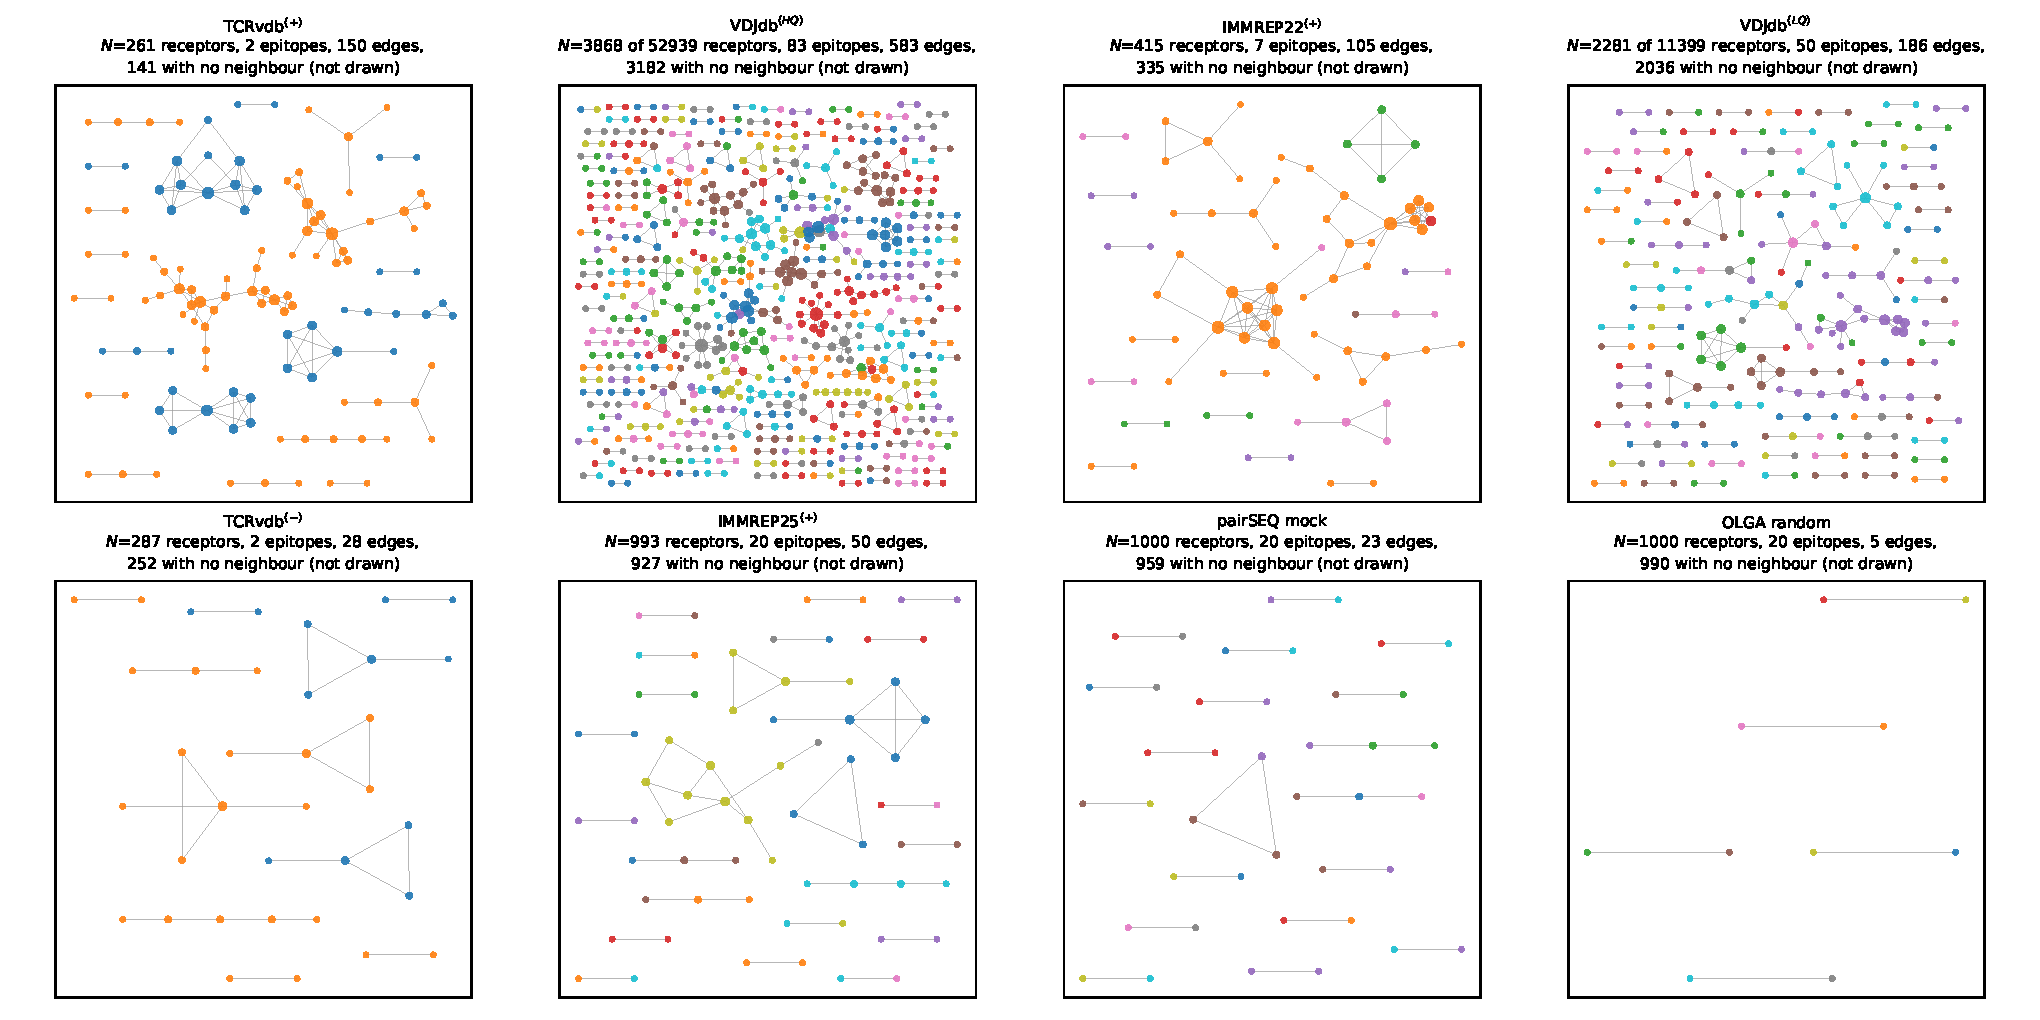
\includegraphics[width=\linewidth]{../results/figures/fig_homology_graph_TRB.pdf}
\caption{TR$\beta$ homology graph per cohort (equal sampling). Edge counts:
VDJdb-HQ $\sim$550, TCRvdb-true 75, versus immrep25 $\sim$17 and OLGA $\sim$1.}
\label{fig:homgraph}
\end{figure}

\section{Pairing test}\label{sec:pairing}

\paragraph{Metric.} Genome-wide $\alpha/\beta$ pairing is close to
random~\cite{Shcherbinin_2020}, but given an epitope the V/J usage is constrained. Two
signals are scored against permutation nulls, per cohort at the matched design:
\begin{itemize}\itemsep2pt
\item \textbf{gene-usage bias}: $\overline{\mathrm{KL}}=\sum_e w_e\,
  \mathrm{KL}\!\left(P_e(\text{gene})\,\|\,Q(\text{gene})\right)$ over axes
  $V\alpha,J\alpha,V\beta,J\beta$, with $P_e$ the within-epitope gene distribution
  and $Q$ the cohort background; null $=$ shuffle epitope labels.
\item \textbf{inter-chain MI}: $\overline{I}=\sum_e w_e\,
  I\!\left((V\alpha,J\alpha);(V\beta,J\beta)\right)$ within epitope
  (Miller--Madow corrected); null $=$ shuffle the $\alpha\!\leftrightarrow\!\beta$
  pairing within each epitope (keeps marginals, destroys coupling).
\end{itemize}
Both are reported as $z=(\text{obs}-\mu_{\text{null}})/\sigma_{\text{null}}$;
signal $\Rightarrow z\gg0$, random $\Rightarrow z\approx0$.

\paragraph{Result.} Figure~\ref{fig:pair} shows both $z$-scores. The verified
cohorts are strongly non-random (VDJdb-HQ gene-bias $z=\hqGeneZ$), while immrep25
positives are at the floor: gene-usage bias $z=\immGeneZ$ and, decisively, an
inter-chain coupling of $z=\immMiZ$---i.e.\ \emph{no} $\alpha$--$\beta$ coupling
beyond marginals, exactly the random-pairing expectation shared with OLGA. (The
large raw MI at $K{=}30$ is finite-sample bias; the pairing-shuffle null removes
it.)

\begin{figure}[h]\centering
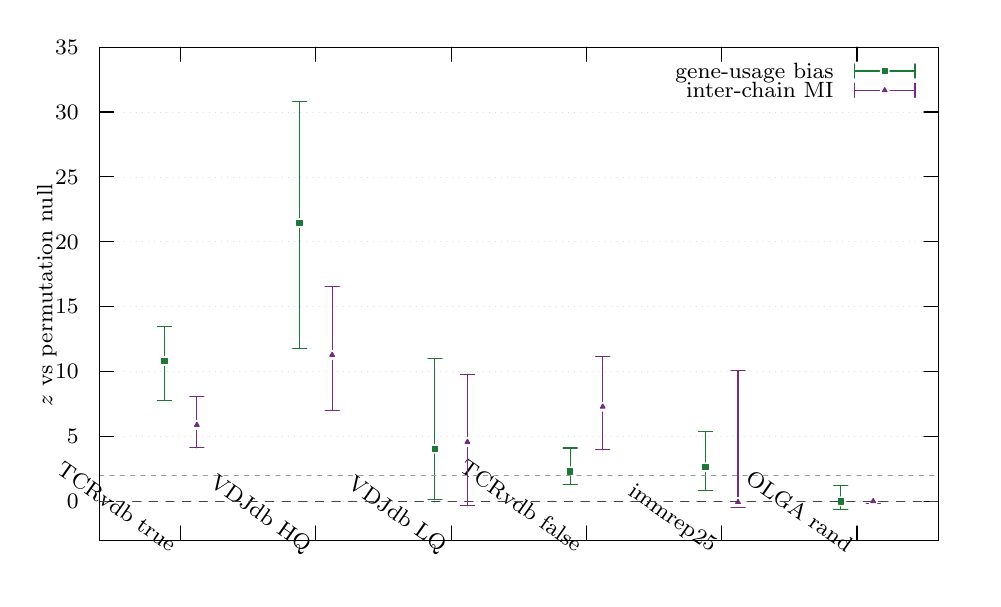
\begin{tikzpicture}[gnuplot]
%% generated with GNUPLOT 6.0p4 (Lua 5.5; terminal rev. Jun 2020, script rev. 120)
%% Fri Jul  3 23:53:18 2026
\tikzset{every node/.append style={font={\fontsize{8.0pt}{9.6pt}\selectfont}}}
\path (0.000,0.000) rectangle (12.000,7.000);
\gpcolor{rgb color={0.867,0.867,0.867}}
\gpsetlinetype{gp lt axes}
\gpsetdashtype{gp dt axes}
\gpsetlinewidth{0.50}
\draw[gp path] (0.907,0.986)--(11.558,0.986);
\gpcolor{color=gp lt color border}
\gpsetlinetype{gp lt border}
\gpsetdashtype{gp dt solid}
\gpsetlinewidth{1.00}
\draw[gp path] (0.907,0.986)--(1.087,0.986);
\draw[gp path] (11.558,0.986)--(11.378,0.986);
\node[gp node right] at (0.760,0.986) {$0$};
\gpcolor{rgb color={0.867,0.867,0.867}}
\gpsetlinetype{gp lt axes}
\gpsetdashtype{gp dt axes}
\gpsetlinewidth{0.50}
\draw[gp path] (0.907,1.810)--(11.558,1.810);
\gpcolor{color=gp lt color border}
\gpsetlinetype{gp lt border}
\gpsetdashtype{gp dt solid}
\gpsetlinewidth{1.00}
\draw[gp path] (0.907,1.810)--(1.087,1.810);
\draw[gp path] (11.558,1.810)--(11.378,1.810);
\node[gp node right] at (0.760,1.810) {$5$};
\gpcolor{rgb color={0.867,0.867,0.867}}
\gpsetlinetype{gp lt axes}
\gpsetdashtype{gp dt axes}
\gpsetlinewidth{0.50}
\draw[gp path] (0.907,2.634)--(11.558,2.634);
\gpcolor{color=gp lt color border}
\gpsetlinetype{gp lt border}
\gpsetdashtype{gp dt solid}
\gpsetlinewidth{1.00}
\draw[gp path] (0.907,2.634)--(1.087,2.634);
\draw[gp path] (11.558,2.634)--(11.378,2.634);
\node[gp node right] at (0.760,2.634) {$10$};
\gpcolor{rgb color={0.867,0.867,0.867}}
\gpsetlinetype{gp lt axes}
\gpsetdashtype{gp dt axes}
\gpsetlinewidth{0.50}
\draw[gp path] (0.907,3.458)--(11.558,3.458);
\gpcolor{color=gp lt color border}
\gpsetlinetype{gp lt border}
\gpsetdashtype{gp dt solid}
\gpsetlinewidth{1.00}
\draw[gp path] (0.907,3.458)--(1.087,3.458);
\draw[gp path] (11.558,3.458)--(11.378,3.458);
\node[gp node right] at (0.760,3.458) {$15$};
\gpcolor{rgb color={0.867,0.867,0.867}}
\gpsetlinetype{gp lt axes}
\gpsetdashtype{gp dt axes}
\gpsetlinewidth{0.50}
\draw[gp path] (0.907,4.282)--(11.558,4.282);
\gpcolor{color=gp lt color border}
\gpsetlinetype{gp lt border}
\gpsetdashtype{gp dt solid}
\gpsetlinewidth{1.00}
\draw[gp path] (0.907,4.282)--(1.087,4.282);
\draw[gp path] (11.558,4.282)--(11.378,4.282);
\node[gp node right] at (0.760,4.282) {$20$};
\gpcolor{rgb color={0.867,0.867,0.867}}
\gpsetlinetype{gp lt axes}
\gpsetdashtype{gp dt axes}
\gpsetlinewidth{0.50}
\draw[gp path] (0.907,5.105)--(11.558,5.105);
\gpcolor{color=gp lt color border}
\gpsetlinetype{gp lt border}
\gpsetdashtype{gp dt solid}
\gpsetlinewidth{1.00}
\draw[gp path] (0.907,5.105)--(1.087,5.105);
\draw[gp path] (11.558,5.105)--(11.378,5.105);
\node[gp node right] at (0.760,5.105) {$25$};
\gpcolor{rgb color={0.867,0.867,0.867}}
\gpsetlinetype{gp lt axes}
\gpsetdashtype{gp dt axes}
\gpsetlinewidth{0.50}
\draw[gp path] (0.907,5.929)--(11.558,5.929);
\gpcolor{color=gp lt color border}
\gpsetlinetype{gp lt border}
\gpsetdashtype{gp dt solid}
\gpsetlinewidth{1.00}
\draw[gp path] (0.907,5.929)--(1.087,5.929);
\draw[gp path] (11.558,5.929)--(11.378,5.929);
\node[gp node right] at (0.760,5.929) {$30$};
\gpcolor{rgb color={0.867,0.867,0.867}}
\gpsetlinetype{gp lt axes}
\gpsetdashtype{gp dt axes}
\gpsetlinewidth{0.50}
\draw[gp path] (0.907,6.753)--(11.558,6.753);
\gpcolor{color=gp lt color border}
\gpsetlinetype{gp lt border}
\gpsetdashtype{gp dt solid}
\gpsetlinewidth{1.00}
\draw[gp path] (0.907,6.753)--(1.087,6.753);
\draw[gp path] (11.558,6.753)--(11.378,6.753);
\node[gp node right] at (0.760,6.753) {$35$};
\draw[gp path] (1.938,0.492)--(1.938,0.672);
\draw[gp path] (1.938,6.753)--(1.938,6.573);
\node[gp node right,rotate=-35.0] at (1.938,0.345) {TCRvdb true};
\draw[gp path] (3.656,0.492)--(3.656,0.672);
\draw[gp path] (3.656,6.753)--(3.656,6.573);
\node[gp node right,rotate=-35.0] at (3.656,0.345) {VDJdb HQ};
\draw[gp path] (5.374,0.492)--(5.374,0.672);
\draw[gp path] (5.374,6.753)--(5.374,6.573);
\node[gp node right,rotate=-35.0] at (5.374,0.345) {VDJdb LQ};
\draw[gp path] (7.091,0.492)--(7.091,0.672);
\draw[gp path] (7.091,6.753)--(7.091,6.573);
\node[gp node right,rotate=-35.0] at (7.091,0.345) {TCRvdb false};
\draw[gp path] (8.809,0.492)--(8.809,0.672);
\draw[gp path] (8.809,6.753)--(8.809,6.573);
\node[gp node right,rotate=-35.0] at (8.809,0.345) {immrep25};
\draw[gp path] (10.527,0.492)--(10.527,0.672);
\draw[gp path] (10.527,6.753)--(10.527,6.573);
\node[gp node right,rotate=-35.0] at (10.527,0.345) {OLGA rand};
\draw[gp path] (0.907,6.753)--(0.907,0.492)--(11.558,0.492)--(11.558,6.753)--cycle;
\node[gp node right] at (10.349,6.450) {gene-usage bias};
\gpcolor{rgb color={0.106,0.471,0.216}}
\draw[gp path] (10.496,6.450)--(11.264,6.450);
\draw[gp path] (10.496,6.540)--(10.496,6.360);
\draw[gp path] (11.264,6.540)--(11.264,6.360);
\draw[gp path] (1.732,2.268)--(1.732,3.200);
\draw[gp path] (1.642,2.268)--(1.822,2.268);
\draw[gp path] (1.642,3.200)--(1.822,3.200);
\draw[gp path] (3.449,2.920)--(3.449,6.059);
\draw[gp path] (3.359,2.920)--(3.539,2.920);
\draw[gp path] (3.359,6.059)--(3.539,6.059);
\draw[gp path] (5.167,1.003)--(5.167,2.798);
\draw[gp path] (5.077,1.003)--(5.257,1.003);
\draw[gp path] (5.077,2.798)--(5.257,2.798);
\draw[gp path] (6.885,1.198)--(6.885,1.662);
\draw[gp path] (6.795,1.198)--(6.975,1.198);
\draw[gp path] (6.795,1.662)--(6.975,1.662);
\draw[gp path] (8.603,1.123)--(8.603,1.869);
\draw[gp path] (8.513,1.123)--(8.693,1.123);
\draw[gp path] (8.513,1.869)--(8.693,1.869);
\draw[gp path] (10.321,0.878)--(10.321,1.188);
\draw[gp path] (10.231,0.878)--(10.411,0.878);
\draw[gp path] (10.231,1.188)--(10.411,1.188);
\gpcolor{color=gpbgfillcolor}
\gpsetpointsize{4.00}
\gp3point{gp mark 7}{}{(1.732,2.769)}
\gpcolor{rgb color={0.106,0.471,0.216}}
\gpsetpointsize{2.40}
\gp3point{gp mark 5}{}{(1.732,2.769)}
\gpcolor{color=gpbgfillcolor}
\gpsetpointsize{4.00}
\gp3point{gp mark 7}{}{(3.449,4.519)}
\gpcolor{rgb color={0.106,0.471,0.216}}
\gpsetpointsize{2.40}
\gp3point{gp mark 5}{}{(3.449,4.519)}
\gpcolor{color=gpbgfillcolor}
\gpsetpointsize{4.00}
\gp3point{gp mark 7}{}{(5.167,1.652)}
\gpcolor{rgb color={0.106,0.471,0.216}}
\gpsetpointsize{2.40}
\gp3point{gp mark 5}{}{(5.167,1.652)}
\gpcolor{color=gpbgfillcolor}
\gpsetpointsize{4.00}
\gp3point{gp mark 7}{}{(6.885,1.366)}
\gpcolor{rgb color={0.106,0.471,0.216}}
\gpsetpointsize{2.40}
\gp3point{gp mark 5}{}{(6.885,1.366)}
\gpcolor{color=gpbgfillcolor}
\gpsetpointsize{4.00}
\gp3point{gp mark 7}{}{(8.603,1.418)}
\gpcolor{rgb color={0.106,0.471,0.216}}
\gpsetpointsize{2.40}
\gp3point{gp mark 5}{}{(8.603,1.418)}
\gpcolor{color=gpbgfillcolor}
\gpsetpointsize{4.00}
\gp3point{gp mark 7}{}{(10.321,0.984)}
\gpcolor{rgb color={0.106,0.471,0.216}}
\gpsetpointsize{2.40}
\gp3point{gp mark 5}{}{(10.321,0.984)}
\gpcolor{color=gpbgfillcolor}
\gpsetpointsize{4.00}
\gp3point{gp mark 7}{}{(10.880,6.450)}
\gpcolor{rgb color={0.106,0.471,0.216}}
\gpsetpointsize{2.40}
\gp3point{gp mark 5}{}{(10.880,6.450)}
\gpcolor{color=gp lt color border}
\node[gp node right] at (10.349,6.204) {inter-chain MI};
\gpcolor{rgb color={0.463,0.165,0.514}}
\draw[gp path] (10.496,6.204)--(11.264,6.204);
\draw[gp path] (10.496,6.294)--(10.496,6.114);
\draw[gp path] (11.264,6.294)--(11.264,6.114);
\draw[gp path] (2.144,1.663)--(2.144,2.315);
\draw[gp path] (2.054,1.663)--(2.234,1.663);
\draw[gp path] (2.054,2.315)--(2.234,2.315);
\draw[gp path] (3.862,2.140)--(3.862,3.711);
\draw[gp path] (3.772,2.140)--(3.952,2.140);
\draw[gp path] (3.772,3.711)--(3.952,3.711);
\draw[gp path] (5.580,0.928)--(5.580,2.598);
\draw[gp path] (5.490,0.928)--(5.670,0.928);
\draw[gp path] (5.490,2.598)--(5.670,2.598);
\draw[gp path] (7.298,1.638)--(7.298,2.819);
\draw[gp path] (7.208,1.638)--(7.388,1.638);
\draw[gp path] (7.208,2.819)--(7.388,2.819);
\draw[gp path] (9.016,0.907)--(9.016,2.643);
\draw[gp path] (8.926,0.907)--(9.106,0.907);
\draw[gp path] (8.926,2.643)--(9.106,2.643);
\draw[gp path] (10.733,0.960)--(10.733,0.986);
\draw[gp path] (10.643,0.960)--(10.823,0.960);
\draw[gp path] (10.643,0.986)--(10.823,0.986);
\gpcolor{color=gpbgfillcolor}
\gpsetpointsize{4.00}
\gp3point{gp mark 7}{}{(2.144,1.955)}
\gpcolor{rgb color={0.463,0.165,0.514}}
\gpsetpointsize{2.40}
\gp3point{gp mark 9}{}{(2.144,1.955)}
\gpcolor{color=gpbgfillcolor}
\gpsetpointsize{4.00}
\gp3point{gp mark 7}{}{(3.862,2.844)}
\gpcolor{rgb color={0.463,0.165,0.514}}
\gpsetpointsize{2.40}
\gp3point{gp mark 9}{}{(3.862,2.844)}
\gpcolor{color=gpbgfillcolor}
\gpsetpointsize{4.00}
\gp3point{gp mark 7}{}{(5.580,1.739)}
\gpcolor{rgb color={0.463,0.165,0.514}}
\gpsetpointsize{2.40}
\gp3point{gp mark 9}{}{(5.580,1.739)}
\gpcolor{color=gpbgfillcolor}
\gpsetpointsize{4.00}
\gp3point{gp mark 7}{}{(7.298,2.186)}
\gpcolor{rgb color={0.463,0.165,0.514}}
\gpsetpointsize{2.40}
\gp3point{gp mark 9}{}{(7.298,2.186)}
\gpcolor{color=gpbgfillcolor}
\gpsetpointsize{4.00}
\gp3point{gp mark 7}{}{(9.016,0.976)}
\gpcolor{rgb color={0.463,0.165,0.514}}
\gpsetpointsize{2.40}
\gp3point{gp mark 9}{}{(9.016,0.976)}
\gpcolor{color=gpbgfillcolor}
\gpsetpointsize{4.00}
\gp3point{gp mark 7}{}{(10.733,0.986)}
\gpcolor{rgb color={0.463,0.165,0.514}}
\gpsetpointsize{2.40}
\gp3point{gp mark 9}{}{(10.733,0.986)}
\gpcolor{color=gpbgfillcolor}
\gpsetpointsize{4.00}
\gp3point{gp mark 7}{}{(10.880,6.204)}
\gpcolor{rgb color={0.463,0.165,0.514}}
\gpsetpointsize{2.40}
\gp3point{gp mark 9}{}{(10.880,6.204)}
\gpcolor{rgb color={0.267,0.267,0.267}}
\gpsetdashtype{gp dt 2}
\draw[gp path] (0.907,0.986)--(1.015,0.986)--(1.122,0.986)--(1.230,0.986)--(1.337,0.986)%
  --(1.445,0.986)--(1.553,0.986)--(1.660,0.986)--(1.768,0.986)--(1.875,0.986)--(1.983,0.986)%
  --(2.090,0.986)--(2.198,0.986)--(2.306,0.986)--(2.413,0.986)--(2.521,0.986)--(2.628,0.986)%
  --(2.736,0.986)--(2.844,0.986)--(2.951,0.986)--(3.059,0.986)--(3.166,0.986)--(3.274,0.986)%
  --(3.381,0.986)--(3.489,0.986)--(3.597,0.986)--(3.704,0.986)--(3.812,0.986)--(3.919,0.986)%
  --(4.027,0.986)--(4.135,0.986)--(4.242,0.986)--(4.350,0.986)--(4.457,0.986)--(4.565,0.986)%
  --(4.673,0.986)--(4.780,0.986)--(4.888,0.986)--(4.995,0.986)--(5.103,0.986)--(5.210,0.986)%
  --(5.318,0.986)--(5.426,0.986)--(5.533,0.986)--(5.641,0.986)--(5.748,0.986)--(5.856,0.986)%
  --(5.964,0.986)--(6.071,0.986)--(6.179,0.986)--(6.286,0.986)--(6.394,0.986)--(6.501,0.986)%
  --(6.609,0.986)--(6.717,0.986)--(6.824,0.986)--(6.932,0.986)--(7.039,0.986)--(7.147,0.986)%
  --(7.255,0.986)--(7.362,0.986)--(7.470,0.986)--(7.577,0.986)--(7.685,0.986)--(7.792,0.986)%
  --(7.900,0.986)--(8.008,0.986)--(8.115,0.986)--(8.223,0.986)--(8.330,0.986)--(8.438,0.986)%
  --(8.546,0.986)--(8.653,0.986)--(8.761,0.986)--(8.868,0.986)--(8.976,0.986)--(9.084,0.986)%
  --(9.191,0.986)--(9.299,0.986)--(9.406,0.986)--(9.514,0.986)--(9.621,0.986)--(9.729,0.986)%
  --(9.837,0.986)--(9.944,0.986)--(10.052,0.986)--(10.159,0.986)--(10.267,0.986)--(10.375,0.986)%
  --(10.482,0.986)--(10.590,0.986)--(10.697,0.986)--(10.805,0.986)--(10.912,0.986)--(11.020,0.986)%
  --(11.128,0.986)--(11.235,0.986)--(11.343,0.986)--(11.450,0.986)--(11.558,0.986);
\gpcolor{rgb color={0.600,0.600,0.600}}
\gpsetdashtype{gp dt 3}
\draw[gp path] (0.907,1.316)--(1.015,1.316)--(1.122,1.316)--(1.230,1.316)--(1.337,1.316)%
  --(1.445,1.316)--(1.553,1.316)--(1.660,1.316)--(1.768,1.316)--(1.875,1.316)--(1.983,1.316)%
  --(2.090,1.316)--(2.198,1.316)--(2.306,1.316)--(2.413,1.316)--(2.521,1.316)--(2.628,1.316)%
  --(2.736,1.316)--(2.844,1.316)--(2.951,1.316)--(3.059,1.316)--(3.166,1.316)--(3.274,1.316)%
  --(3.381,1.316)--(3.489,1.316)--(3.597,1.316)--(3.704,1.316)--(3.812,1.316)--(3.919,1.316)%
  --(4.027,1.316)--(4.135,1.316)--(4.242,1.316)--(4.350,1.316)--(4.457,1.316)--(4.565,1.316)%
  --(4.673,1.316)--(4.780,1.316)--(4.888,1.316)--(4.995,1.316)--(5.103,1.316)--(5.210,1.316)%
  --(5.318,1.316)--(5.426,1.316)--(5.533,1.316)--(5.641,1.316)--(5.748,1.316)--(5.856,1.316)%
  --(5.964,1.316)--(6.071,1.316)--(6.179,1.316)--(6.286,1.316)--(6.394,1.316)--(6.501,1.316)%
  --(6.609,1.316)--(6.717,1.316)--(6.824,1.316)--(6.932,1.316)--(7.039,1.316)--(7.147,1.316)%
  --(7.255,1.316)--(7.362,1.316)--(7.470,1.316)--(7.577,1.316)--(7.685,1.316)--(7.792,1.316)%
  --(7.900,1.316)--(8.008,1.316)--(8.115,1.316)--(8.223,1.316)--(8.330,1.316)--(8.438,1.316)%
  --(8.546,1.316)--(8.653,1.316)--(8.761,1.316)--(8.868,1.316)--(8.976,1.316)--(9.084,1.316)%
  --(9.191,1.316)--(9.299,1.316)--(9.406,1.316)--(9.514,1.316)--(9.621,1.316)--(9.729,1.316)%
  --(9.837,1.316)--(9.944,1.316)--(10.052,1.316)--(10.159,1.316)--(10.267,1.316)--(10.375,1.316)%
  --(10.482,1.316)--(10.590,1.316)--(10.697,1.316)--(10.805,1.316)--(10.912,1.316)--(11.020,1.316)%
  --(11.128,1.316)--(11.235,1.316)--(11.343,1.316)--(11.450,1.316)--(11.558,1.316);
\gpcolor{color=gp lt color border}
\gpsetdashtype{gp dt solid}
\draw[gp path] (0.907,6.753)--(0.907,0.492)--(11.558,0.492)--(11.558,6.753)--cycle;
\node[gp node center,rotate=-270.0] at (0.232,3.622) {$z$ vs permutation null};
%% coordinates of the plot area
\gpdefrectangularnode{gp plot 1}{\pgfpoint{0.907cm}{0.492cm}}{\pgfpoint{11.558cm}{6.753cm}}
\end{tikzpicture}
%% gnuplot variables

\caption{Pairing non-randomness $z$ (median, 95\% CI) per cohort: gene-usage bias
(squares) and inter-chain mutual information (triangles). Dashed line $z{=}0$
(random), dotted $z{=}2$. immrep25 and OLGA sit at the random line on both.}
\label{fig:pair}
\end{figure}

\section{Publicity control}\label{sec:publicity}

The one alternative to ``pure noise'' is \emph{publicity}: immrep25 might reuse
public TCRs whose chance homology mimics epitope signal. Although only $0.3\%$ of
positives share \emph{both} chains exactly with VDJdb, allowing a single
substitution and either chain, $\pubAny\%$ of immrep25 positives are within
Hamming $\le 1$ of a known VDJdb/TCRvdb TCR ($\pubA\%$ on $\alpha$, $\pubB\%$ on
$\beta$)---the $\alpha$ chain being especially germline-public. Consistently, the
positives are enriched for high generation probability relative to raw OLGA
sampling (Fig.~\ref{fig:pgen}), i.e.\ they are ``easy-to-generate'', public-leaning
sequences; this is exactly why the random control must be $P_{\text{gen}}$-matched.

Removing public positives collapses the (already weak) homology to the noise floor:
one-vs-many S/N falls from $\immHomB$ to $\npHomB$ on TR$\beta$ and from $\immHomA$ to
$\npHomA$ on TR$\alpha$ (Fig.~\ref{fig:pub}). The residual signal was therefore
publicity, not epitope-specific convergence.

\begin{figure}[h]\centering
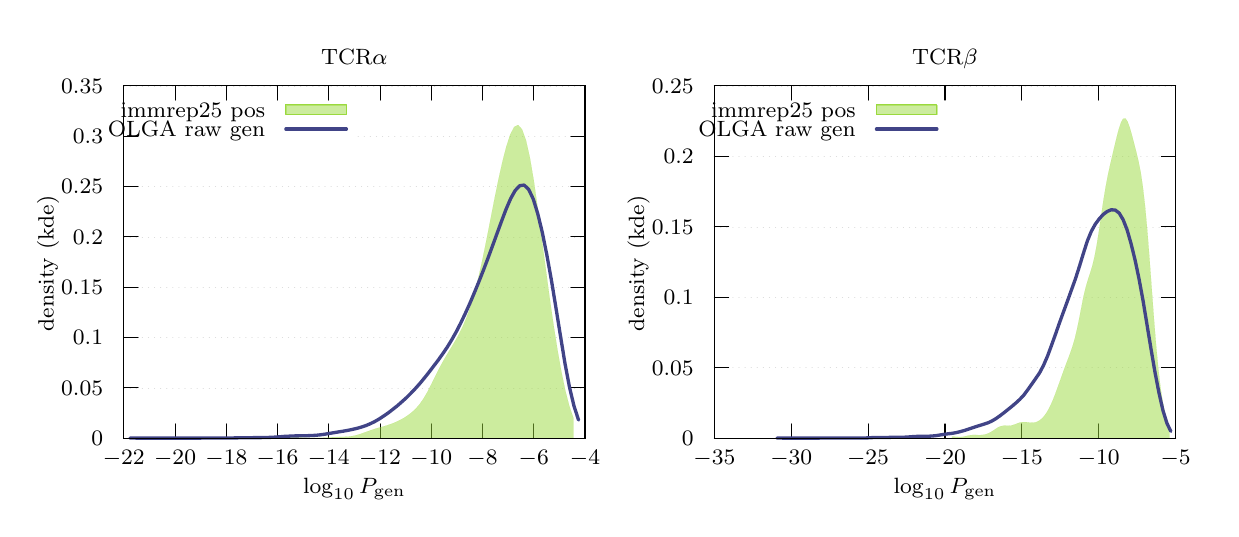
\begin{tikzpicture}[gnuplot]
%% generated with GNUPLOT 6.0p4 (Lua 5.5; terminal rev. Jun 2020, script rev. 120)
%% Sat Jul  4 05:10:26 2026
\tikzset{every node/.append style={font={\fontsize{8.0pt}{9.6pt}\selectfont}}}
\path (0.000,0.000) rectangle (15.000,6.000);
\gpcolor{rgb color={0.867,0.867,0.867}}
\gpsetlinetype{gp lt axes}
\gpsetdashtype{gp dt axes}
\gpsetlinewidth{0.50}
\draw[gp path] (1.201,0.787)--(7.058,0.787);
\gpcolor{color=gp lt color border}
\gpsetlinetype{gp lt border}
\gpsetdashtype{gp dt solid}
\gpsetlinewidth{1.00}
\draw[gp path] (1.201,0.787)--(1.381,0.787);
\draw[gp path] (7.058,0.787)--(6.878,0.787);
\node[gp node right] at (1.054,0.787) {$0$};
\gpcolor{rgb color={0.867,0.867,0.867}}
\gpsetlinetype{gp lt axes}
\gpsetdashtype{gp dt axes}
\gpsetlinewidth{0.50}
\draw[gp path] (1.201,1.426)--(7.058,1.426);
\gpcolor{color=gp lt color border}
\gpsetlinetype{gp lt border}
\gpsetdashtype{gp dt solid}
\gpsetlinewidth{1.00}
\draw[gp path] (1.201,1.426)--(1.381,1.426);
\draw[gp path] (7.058,1.426)--(6.878,1.426);
\node[gp node right] at (1.054,1.426) {$0.05$};
\gpcolor{rgb color={0.867,0.867,0.867}}
\gpsetlinetype{gp lt axes}
\gpsetdashtype{gp dt axes}
\gpsetlinewidth{0.50}
\draw[gp path] (1.201,2.065)--(7.058,2.065);
\gpcolor{color=gp lt color border}
\gpsetlinetype{gp lt border}
\gpsetdashtype{gp dt solid}
\gpsetlinewidth{1.00}
\draw[gp path] (1.201,2.065)--(1.381,2.065);
\draw[gp path] (7.058,2.065)--(6.878,2.065);
\node[gp node right] at (1.054,2.065) {$0.1$};
\gpcolor{rgb color={0.867,0.867,0.867}}
\gpsetlinetype{gp lt axes}
\gpsetdashtype{gp dt axes}
\gpsetlinewidth{0.50}
\draw[gp path] (1.201,2.704)--(7.058,2.704);
\gpcolor{color=gp lt color border}
\gpsetlinetype{gp lt border}
\gpsetdashtype{gp dt solid}
\gpsetlinewidth{1.00}
\draw[gp path] (1.201,2.704)--(1.381,2.704);
\draw[gp path] (7.058,2.704)--(6.878,2.704);
\node[gp node right] at (1.054,2.704) {$0.15$};
\gpcolor{rgb color={0.867,0.867,0.867}}
\gpsetlinetype{gp lt axes}
\gpsetdashtype{gp dt axes}
\gpsetlinewidth{0.50}
\draw[gp path] (1.201,3.344)--(7.058,3.344);
\gpcolor{color=gp lt color border}
\gpsetlinetype{gp lt border}
\gpsetdashtype{gp dt solid}
\gpsetlinewidth{1.00}
\draw[gp path] (1.201,3.344)--(1.381,3.344);
\draw[gp path] (7.058,3.344)--(6.878,3.344);
\node[gp node right] at (1.054,3.344) {$0.2$};
\gpcolor{rgb color={0.867,0.867,0.867}}
\gpsetlinetype{gp lt axes}
\gpsetdashtype{gp dt axes}
\gpsetlinewidth{0.50}
\draw[gp path] (1.201,3.983)--(7.058,3.983);
\gpcolor{color=gp lt color border}
\gpsetlinetype{gp lt border}
\gpsetdashtype{gp dt solid}
\gpsetlinewidth{1.00}
\draw[gp path] (1.201,3.983)--(1.381,3.983);
\draw[gp path] (7.058,3.983)--(6.878,3.983);
\node[gp node right] at (1.054,3.983) {$0.25$};
\gpcolor{rgb color={0.867,0.867,0.867}}
\gpsetlinetype{gp lt axes}
\gpsetdashtype{gp dt axes}
\gpsetlinewidth{0.50}
\draw[gp path] (1.201,4.622)--(1.348,4.622);
\draw[gp path] (4.174,4.622)--(7.058,4.622);
\gpcolor{color=gp lt color border}
\gpsetlinetype{gp lt border}
\gpsetdashtype{gp dt solid}
\gpsetlinewidth{1.00}
\draw[gp path] (1.201,4.622)--(1.381,4.622);
\draw[gp path] (7.058,4.622)--(6.878,4.622);
\node[gp node right] at (1.054,4.622) {$0.3$};
\gpcolor{rgb color={0.867,0.867,0.867}}
\gpsetlinetype{gp lt axes}
\gpsetdashtype{gp dt axes}
\gpsetlinewidth{0.50}
\draw[gp path] (1.201,5.261)--(7.058,5.261);
\gpcolor{color=gp lt color border}
\gpsetlinetype{gp lt border}
\gpsetdashtype{gp dt solid}
\gpsetlinewidth{1.00}
\draw[gp path] (1.201,5.261)--(1.381,5.261);
\draw[gp path] (7.058,5.261)--(6.878,5.261);
\node[gp node right] at (1.054,5.261) {$0.35$};
\draw[gp path] (1.201,0.787)--(1.201,0.967);
\draw[gp path] (1.201,5.261)--(1.201,5.081);
\node[gp node center] at (1.201,0.541) {$-22$};
\draw[gp path] (1.852,0.787)--(1.852,0.967);
\draw[gp path] (1.852,5.261)--(1.852,5.081);
\node[gp node center] at (1.852,0.541) {$-20$};
\draw[gp path] (2.503,0.787)--(2.503,0.967);
\draw[gp path] (2.503,5.261)--(2.503,5.081);
\node[gp node center] at (2.503,0.541) {$-18$};
\draw[gp path] (3.153,0.787)--(3.153,0.967);
\draw[gp path] (3.153,5.261)--(3.153,5.081);
\node[gp node center] at (3.153,0.541) {$-16$};
\draw[gp path] (3.804,0.787)--(3.804,0.967);
\draw[gp path] (3.804,5.261)--(3.804,5.081);
\node[gp node center] at (3.804,0.541) {$-14$};
\draw[gp path] (4.455,0.787)--(4.455,0.967);
\draw[gp path] (4.455,5.261)--(4.455,5.081);
\node[gp node center] at (4.455,0.541) {$-12$};
\draw[gp path] (5.106,0.787)--(5.106,0.967);
\draw[gp path] (5.106,5.261)--(5.106,5.081);
\node[gp node center] at (5.106,0.541) {$-10$};
\draw[gp path] (5.756,0.787)--(5.756,0.967);
\draw[gp path] (5.756,5.261)--(5.756,5.081);
\node[gp node center] at (5.756,0.541) {$-8$};
\draw[gp path] (6.407,0.787)--(6.407,0.967);
\draw[gp path] (6.407,5.261)--(6.407,5.081);
\node[gp node center] at (6.407,0.541) {$-6$};
\draw[gp path] (7.058,0.787)--(7.058,0.967);
\draw[gp path] (7.058,5.261)--(7.058,5.081);
\node[gp node center] at (7.058,0.541) {$-4$};
\draw[gp path] (1.201,5.261)--(1.201,0.787)--(7.058,0.787)--(7.058,5.261)--cycle;
\node[gp node right] at (3.112,4.958) {immrep25 pos};
\gpfill{rgb color={0.603,0.850,0.238},opacity=0.50} (3.259,4.897)--(4.027,4.897)--(4.027,5.020)--(3.259,5.020)--cycle;
\gpcolor{rgb color={0.603,0.850,0.238}}
\draw[gp path] (3.259,4.897)--(4.027,4.897)--(4.027,5.019)--(3.259,5.019)--cycle;
\gpfill{rgb color={0.603,0.850,0.238},opacity=0.50} (1.956,0.800)--(2.006,0.799)--(2.056,0.796)--(2.106,0.794)%
    --(2.156,0.791)--(2.206,0.789)--(2.256,0.788)--(2.306,0.787)--(2.356,0.787)%
    --(2.406,0.787)--(2.456,0.787)--(2.506,0.787)--(2.556,0.787)--(2.606,0.787)%
    --(2.657,0.787)--(2.707,0.787)--(2.757,0.788)--(2.807,0.788)--(2.857,0.790)%
    --(2.907,0.792)--(2.957,0.796)--(3.007,0.799)--(3.057,0.801)--(3.107,0.803)%
    --(3.157,0.803)--(3.207,0.803)--(3.257,0.803)--(3.307,0.802)--(3.357,0.801)%
    --(3.407,0.798)--(3.457,0.795)--(3.507,0.792)--(3.557,0.790)--(3.607,0.789)%
    --(3.657,0.789)--(3.707,0.790)--(3.757,0.793)--(3.807,0.796)--(3.857,0.799)%
    --(3.907,0.801)--(3.957,0.802)--(4.007,0.804)--(4.057,0.807)--(4.107,0.814)%
    --(4.157,0.825)--(4.207,0.840)--(4.257,0.858)--(4.307,0.876)--(4.357,0.894)%
    --(4.407,0.910)--(4.457,0.924)--(4.507,0.938)--(4.557,0.954)--(4.608,0.971)%
    --(4.658,0.992)--(4.708,1.016)--(4.758,1.043)--(4.808,1.076)--(4.858,1.114)%
    --(4.908,1.160)--(4.958,1.218)--(5.008,1.290)--(5.058,1.376)--(5.108,1.474)%
    --(5.158,1.576)--(5.208,1.675)--(5.258,1.767)--(5.308,1.853)--(5.358,1.935)%
    --(5.408,2.019)--(5.458,2.109)--(5.508,2.211)--(5.558,2.331)--(5.608,2.474)%
    --(5.658,2.645)--(5.708,2.843)--(5.758,3.068)--(5.808,3.313)--(5.858,3.568)%
    --(5.908,3.824)--(5.958,4.069)--(6.008,4.293)--(6.058,4.488)--(6.108,4.641)%
    --(6.158,4.738)--(6.208,4.763)--(6.258,4.708)--(6.308,4.569)--(6.358,4.347)%
    --(6.408,4.052)--(6.458,3.702)--(6.508,3.322)--(6.559,2.937)--(6.609,2.565)%
    --(6.659,2.219)--(6.709,1.903)--(6.759,1.623)--(6.809,1.385)--(6.859,1.192)%
    --(6.909,1.046)--(6.909,0.787)--(1.956,0.787)--cycle;
\gpcolor{color=gp lt color border}
\node[gp node right] at (3.112,4.712) {OLGA raw gen};
\gpcolor{rgb color={0.254,0.265,0.530}}
\gpsetlinewidth{3.00}
\draw[gp path] (3.259,4.712)--(4.027,4.712);
\draw[gp path] (1.278,0.788)--(1.335,0.788)--(1.393,0.787)--(1.450,0.787)--(1.508,0.787)%
  --(1.565,0.787)--(1.623,0.787)--(1.680,0.787)--(1.738,0.787)--(1.796,0.787)--(1.853,0.787)%
  --(1.911,0.787)--(1.968,0.787)--(2.026,0.787)--(2.083,0.787)--(2.141,0.787)--(2.199,0.788)%
  --(2.256,0.788)--(2.314,0.788)--(2.371,0.788)--(2.429,0.788)--(2.486,0.789)--(2.544,0.789)%
  --(2.601,0.790)--(2.659,0.791)--(2.717,0.792)--(2.774,0.793)--(2.832,0.793)--(2.889,0.794)%
  --(2.947,0.794)--(3.004,0.795)--(3.062,0.797)--(3.120,0.800)--(3.177,0.804)--(3.235,0.809)%
  --(3.292,0.812)--(3.350,0.815)--(3.407,0.816)--(3.465,0.817)--(3.522,0.818)--(3.580,0.820)%
  --(3.638,0.823)--(3.695,0.829)--(3.753,0.837)--(3.810,0.847)--(3.868,0.856)--(3.925,0.866)%
  --(3.983,0.875)--(4.041,0.885)--(4.098,0.897)--(4.156,0.910)--(4.213,0.926)--(4.271,0.945)%
  --(4.328,0.969)--(4.386,0.997)--(4.443,1.030)--(4.501,1.068)--(4.559,1.108)--(4.616,1.152)%
  --(4.674,1.198)--(4.731,1.248)--(4.789,1.300)--(4.846,1.357)--(4.904,1.418)--(4.962,1.483)%
  --(5.019,1.552)--(5.077,1.625)--(5.134,1.700)--(5.192,1.776)--(5.249,1.856)--(5.307,1.941)%
  --(5.364,2.034)--(5.422,2.137)--(5.480,2.250)--(5.537,2.370)--(5.595,2.498)--(5.652,2.633)%
  --(5.710,2.774)--(5.767,2.919)--(5.825,3.071)--(5.882,3.226)--(5.940,3.385)--(5.998,3.543)%
  --(6.055,3.694)--(6.113,3.828)--(6.170,3.931)--(6.228,3.993)--(6.285,4.001)--(6.343,3.945)%
  --(6.401,3.822)--(6.458,3.636)--(6.516,3.397)--(6.573,3.114)--(6.631,2.794)--(6.688,2.446)%
  --(6.746,2.086)--(6.803,1.738)--(6.861,1.433)--(6.919,1.190)--(6.976,1.017);
\gpcolor{color=gp lt color border}
\gpsetlinewidth{1.00}
\draw[gp path] (1.201,5.261)--(1.201,0.787)--(7.058,0.787)--(7.058,5.261)--cycle;
\node[gp node center,rotate=-270.0] at (0.232,3.024) {density (kde)};
\node[gp node center] at (4.129,0.172) {$\log_{10} P_\mathrm{gen}$};
\node[gp node center] at (4.129,5.630) {TCR$\alpha$};
%% coordinates of the plot area
\gpdefrectangularnode{gp plot 1}{\pgfpoint{1.201cm}{0.787cm}}{\pgfpoint{7.058cm}{5.261cm}}
\gpcolor{rgb color={0.867,0.867,0.867}}
\gpsetlinetype{gp lt axes}
\gpsetdashtype{gp dt axes}
\gpsetlinewidth{0.50}
\draw[gp path] (8.701,0.787)--(14.558,0.787);
\gpcolor{color=gp lt color border}
\gpsetlinetype{gp lt border}
\gpsetdashtype{gp dt solid}
\gpsetlinewidth{1.00}
\draw[gp path] (8.701,0.787)--(8.881,0.787);
\draw[gp path] (14.558,0.787)--(14.378,0.787);
\node[gp node right] at (8.554,0.787) {$0$};
\gpcolor{rgb color={0.867,0.867,0.867}}
\gpsetlinetype{gp lt axes}
\gpsetdashtype{gp dt axes}
\gpsetlinewidth{0.50}
\draw[gp path] (8.701,1.682)--(14.558,1.682);
\gpcolor{color=gp lt color border}
\gpsetlinetype{gp lt border}
\gpsetdashtype{gp dt solid}
\gpsetlinewidth{1.00}
\draw[gp path] (8.701,1.682)--(8.881,1.682);
\draw[gp path] (14.558,1.682)--(14.378,1.682);
\node[gp node right] at (8.554,1.682) {$0.05$};
\gpcolor{rgb color={0.867,0.867,0.867}}
\gpsetlinetype{gp lt axes}
\gpsetdashtype{gp dt axes}
\gpsetlinewidth{0.50}
\draw[gp path] (8.701,2.577)--(14.558,2.577);
\gpcolor{color=gp lt color border}
\gpsetlinetype{gp lt border}
\gpsetdashtype{gp dt solid}
\gpsetlinewidth{1.00}
\draw[gp path] (8.701,2.577)--(8.881,2.577);
\draw[gp path] (14.558,2.577)--(14.378,2.577);
\node[gp node right] at (8.554,2.577) {$0.1$};
\gpcolor{rgb color={0.867,0.867,0.867}}
\gpsetlinetype{gp lt axes}
\gpsetdashtype{gp dt axes}
\gpsetlinewidth{0.50}
\draw[gp path] (8.701,3.471)--(14.558,3.471);
\gpcolor{color=gp lt color border}
\gpsetlinetype{gp lt border}
\gpsetdashtype{gp dt solid}
\gpsetlinewidth{1.00}
\draw[gp path] (8.701,3.471)--(8.881,3.471);
\draw[gp path] (14.558,3.471)--(14.378,3.471);
\node[gp node right] at (8.554,3.471) {$0.15$};
\gpcolor{rgb color={0.867,0.867,0.867}}
\gpsetlinetype{gp lt axes}
\gpsetdashtype{gp dt axes}
\gpsetlinewidth{0.50}
\draw[gp path] (8.701,4.366)--(14.558,4.366);
\gpcolor{color=gp lt color border}
\gpsetlinetype{gp lt border}
\gpsetdashtype{gp dt solid}
\gpsetlinewidth{1.00}
\draw[gp path] (8.701,4.366)--(8.881,4.366);
\draw[gp path] (14.558,4.366)--(14.378,4.366);
\node[gp node right] at (8.554,4.366) {$0.2$};
\gpcolor{rgb color={0.867,0.867,0.867}}
\gpsetlinetype{gp lt axes}
\gpsetdashtype{gp dt axes}
\gpsetlinewidth{0.50}
\draw[gp path] (8.701,5.261)--(14.558,5.261);
\gpcolor{color=gp lt color border}
\gpsetlinetype{gp lt border}
\gpsetdashtype{gp dt solid}
\gpsetlinewidth{1.00}
\draw[gp path] (8.701,5.261)--(8.881,5.261);
\draw[gp path] (14.558,5.261)--(14.378,5.261);
\node[gp node right] at (8.554,5.261) {$0.25$};
\draw[gp path] (8.701,0.787)--(8.701,0.967);
\draw[gp path] (8.701,5.261)--(8.701,5.081);
\node[gp node center] at (8.701,0.541) {$-35$};
\draw[gp path] (9.677,0.787)--(9.677,0.967);
\draw[gp path] (9.677,5.261)--(9.677,5.081);
\node[gp node center] at (9.677,0.541) {$-30$};
\draw[gp path] (10.653,0.787)--(10.653,0.967);
\draw[gp path] (10.653,5.261)--(10.653,5.081);
\node[gp node center] at (10.653,0.541) {$-25$};
\draw[gp path] (11.630,0.787)--(11.630,0.967);
\draw[gp path] (11.630,5.261)--(11.630,5.081);
\node[gp node center] at (11.630,0.541) {$-20$};
\draw[gp path] (12.606,0.787)--(12.606,0.967);
\draw[gp path] (12.606,5.261)--(12.606,5.081);
\node[gp node center] at (12.606,0.541) {$-15$};
\draw[gp path] (13.582,0.787)--(13.582,0.967);
\draw[gp path] (13.582,5.261)--(13.582,5.081);
\node[gp node center] at (13.582,0.541) {$-10$};
\draw[gp path] (14.558,0.787)--(14.558,0.967);
\draw[gp path] (14.558,5.261)--(14.558,5.081);
\node[gp node center] at (14.558,0.541) {$-5$};
\draw[gp path] (8.701,5.261)--(8.701,0.787)--(14.558,0.787)--(14.558,5.261)--cycle;
\node[gp node right] at (10.612,4.958) {immrep25 pos};
\gpfill{rgb color={0.603,0.850,0.238},opacity=0.50} (10.759,4.897)--(11.527,4.897)--(11.527,5.020)--(10.759,5.020)--cycle;
\gpcolor{rgb color={0.603,0.850,0.238}}
\draw[gp path] (10.759,4.897)--(11.527,4.897)--(11.527,5.019)--(10.759,5.019)--cycle;
\gpfill{rgb color={0.603,0.850,0.238},opacity=0.50} (11.717,0.805)--(11.745,0.805)--(11.773,0.803)--(11.801,0.801)%
    --(11.829,0.801)--(11.857,0.804)--(11.885,0.810)--(11.912,0.816)--(11.940,0.822)%
    --(11.968,0.826)--(11.996,0.828)--(12.024,0.827)--(12.052,0.826)--(12.080,0.826)%
    --(12.108,0.828)--(12.136,0.833)--(12.163,0.841)--(12.191,0.853)--(12.219,0.868)%
    --(12.247,0.886)--(12.275,0.905)--(12.303,0.923)--(12.331,0.936)--(12.359,0.943)%
    --(12.387,0.945)--(12.414,0.944)--(12.442,0.944)--(12.470,0.947)--(12.498,0.955)%
    --(12.526,0.965)--(12.554,0.976)--(12.582,0.985)--(12.610,0.990)--(12.638,0.991)%
    --(12.665,0.989)--(12.693,0.986)--(12.721,0.983)--(12.749,0.983)--(12.777,0.987)%
    --(12.805,0.997)--(12.833,1.014)--(12.861,1.037)--(12.889,1.067)--(12.916,1.105)%
    --(12.944,1.151)--(12.972,1.207)--(13.000,1.271)--(13.028,1.343)--(13.056,1.419)%
    --(13.084,1.497)--(13.112,1.575)--(13.139,1.651)--(13.167,1.726)--(13.195,1.800)%
    --(13.223,1.875)--(13.251,1.958)--(13.279,2.055)--(13.307,2.173)--(13.335,2.310)%
    --(13.363,2.455)--(13.390,2.591)--(13.418,2.707)--(13.446,2.801)--(13.474,2.886)%
    --(13.502,2.979)--(13.530,3.097)--(13.558,3.248)--(13.586,3.426)--(13.614,3.617)%
    --(13.641,3.804)--(13.669,3.973)--(13.697,4.120)--(13.725,4.249)--(13.753,4.369)%
    --(13.781,4.488)--(13.809,4.605)--(13.837,4.712)--(13.865,4.796)--(13.892,4.844)%
    --(13.920,4.847)--(13.948,4.807)--(13.976,4.730)--(14.004,4.632)--(14.032,4.525)%
    --(14.060,4.416)--(14.088,4.298)--(14.116,4.156)--(14.143,3.970)--(14.171,3.726)%
    --(14.199,3.420)--(14.227,3.064)--(14.255,2.681)--(14.283,2.304)--(14.311,1.959)%
    --(14.339,1.667)--(14.366,1.432)--(14.394,1.250)--(14.422,1.113)--(14.450,1.011)%
    --(14.478,0.936)--(14.478,0.787)--(11.717,0.787)--cycle;
\gpcolor{color=gp lt color border}
\node[gp node right] at (10.612,4.712) {OLGA raw gen};
\gpcolor{rgb color={0.254,0.265,0.530}}
\gpsetlinewidth{3.00}
\draw[gp path] (10.759,4.712)--(11.527,4.712);
\draw[gp path] (9.495,0.788)--(9.546,0.788)--(9.596,0.787)--(9.647,0.787)--(9.697,0.787)%
  --(9.748,0.787)--(9.799,0.787)--(9.849,0.787)--(9.900,0.787)--(9.950,0.787)--(10.001,0.787)%
  --(10.051,0.788)--(10.102,0.788)--(10.152,0.788)--(10.203,0.788)--(10.253,0.788)--(10.304,0.788)%
  --(10.354,0.789)--(10.405,0.789)--(10.456,0.788)--(10.506,0.788)--(10.557,0.788)--(10.607,0.789)%
  --(10.658,0.791)--(10.708,0.794)--(10.759,0.795)--(10.809,0.795)--(10.860,0.795)--(10.910,0.796)%
  --(10.961,0.798)--(11.011,0.798)--(11.062,0.798)--(11.113,0.799)--(11.163,0.802)--(11.214,0.806)%
  --(11.264,0.809)--(11.315,0.810)--(11.365,0.810)--(11.416,0.811)--(11.466,0.814)--(11.517,0.819)%
  --(11.567,0.827)--(11.618,0.835)--(11.668,0.842)--(11.719,0.848)--(11.770,0.857)--(11.820,0.869)%
  --(11.871,0.883)--(11.921,0.899)--(11.972,0.916)--(12.022,0.933)--(12.073,0.949)--(12.123,0.964)%
  --(12.174,0.981)--(12.224,1.004)--(12.275,1.034)--(12.325,1.069)--(12.376,1.108)--(12.426,1.148)%
  --(12.477,1.189)--(12.528,1.232)--(12.578,1.278)--(12.629,1.332)--(12.679,1.399)--(12.730,1.471)%
  --(12.780,1.542)--(12.831,1.617)--(12.881,1.712)--(12.932,1.830)--(12.982,1.965)--(13.033,2.107)%
  --(13.083,2.250)--(13.134,2.390)--(13.185,2.529)--(13.235,2.668)--(13.286,2.810)--(13.336,2.966)%
  --(13.387,3.133)--(13.437,3.290)--(13.488,3.414)--(13.538,3.504)--(13.589,3.573)--(13.639,3.628)%
  --(13.690,3.666)--(13.740,3.687)--(13.791,3.684)--(13.842,3.645)--(13.892,3.561)--(13.943,3.430)%
  --(13.993,3.255)--(14.044,3.047)--(14.094,2.808)--(14.145,2.532)--(14.195,2.228)--(14.246,1.919)%
  --(14.296,1.626)--(14.347,1.362)--(14.397,1.141)--(14.448,0.976)--(14.498,0.873);
\gpcolor{color=gp lt color border}
\gpsetlinewidth{1.00}
\draw[gp path] (8.701,5.261)--(8.701,0.787)--(14.558,0.787)--(14.558,5.261)--cycle;
\node[gp node center,rotate=-270.0] at (7.732,3.024) {density (kde)};
\node[gp node center] at (11.629,0.172) {$\log_{10} P_\mathrm{gen}$};
\node[gp node center] at (11.629,5.630) {TCR$\beta$};
%% coordinates of the plot area
\gpdefrectangularnode{gp plot 2}{\pgfpoint{8.701cm}{0.787cm}}{\pgfpoint{14.558cm}{5.261cm}}
\end{tikzpicture}
%% gnuplot variables

\caption{Per-chain $\log_{10}P_{\text{gen}}$ (kernel density): immrep25 positives
(filled) vs.\ raw OLGA generation (line). Positives skew to higher $P_{\text{gen}}$
(public-leaning), motivating the $P_{\text{gen}}$-matched control.}
\label{fig:pgen}
\end{figure}

\begin{figure}[h]\centering
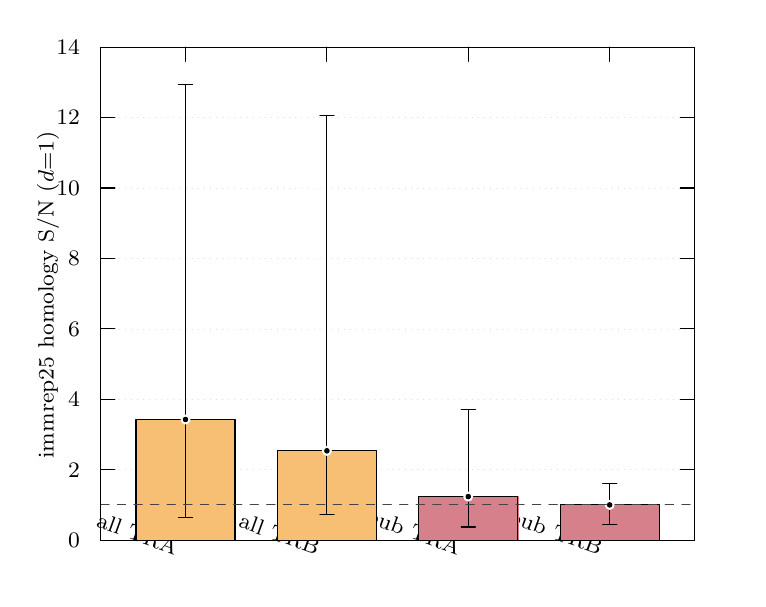
\begin{tikzpicture}[gnuplot]
%% generated with GNUPLOT 6.0p4 (Lua 5.5; terminal rev. Jun 2020, script rev. 120)
%% Fri Jul  3 23:53:18 2026
\tikzset{every node/.append style={font={\fontsize{8.0pt}{9.6pt}\selectfont}}}
\path (0.000,0.000) rectangle (9.000,7.000);
\gpcolor{rgb color={0.867,0.867,0.867}}
\gpsetlinetype{gp lt axes}
\gpsetdashtype{gp dt axes}
\gpsetlinewidth{0.50}
\draw[gp path] (0.907,0.492)--(8.448,0.492);
\gpcolor{color=gp lt color border}
\gpsetlinetype{gp lt border}
\gpsetdashtype{gp dt solid}
\gpsetlinewidth{1.00}
\draw[gp path] (0.907,0.492)--(1.087,0.492);
\draw[gp path] (8.448,0.492)--(8.268,0.492);
\node[gp node right] at (0.760,0.492) {$0$};
\gpcolor{rgb color={0.867,0.867,0.867}}
\gpsetlinetype{gp lt axes}
\gpsetdashtype{gp dt axes}
\gpsetlinewidth{0.50}
\draw[gp path] (0.907,1.386)--(8.448,1.386);
\gpcolor{color=gp lt color border}
\gpsetlinetype{gp lt border}
\gpsetdashtype{gp dt solid}
\gpsetlinewidth{1.00}
\draw[gp path] (0.907,1.386)--(1.087,1.386);
\draw[gp path] (8.448,1.386)--(8.268,1.386);
\node[gp node right] at (0.760,1.386) {$2$};
\gpcolor{rgb color={0.867,0.867,0.867}}
\gpsetlinetype{gp lt axes}
\gpsetdashtype{gp dt axes}
\gpsetlinewidth{0.50}
\draw[gp path] (0.907,2.281)--(8.448,2.281);
\gpcolor{color=gp lt color border}
\gpsetlinetype{gp lt border}
\gpsetdashtype{gp dt solid}
\gpsetlinewidth{1.00}
\draw[gp path] (0.907,2.281)--(1.087,2.281);
\draw[gp path] (8.448,2.281)--(8.268,2.281);
\node[gp node right] at (0.760,2.281) {$4$};
\gpcolor{rgb color={0.867,0.867,0.867}}
\gpsetlinetype{gp lt axes}
\gpsetdashtype{gp dt axes}
\gpsetlinewidth{0.50}
\draw[gp path] (0.907,3.175)--(8.448,3.175);
\gpcolor{color=gp lt color border}
\gpsetlinetype{gp lt border}
\gpsetdashtype{gp dt solid}
\gpsetlinewidth{1.00}
\draw[gp path] (0.907,3.175)--(1.087,3.175);
\draw[gp path] (8.448,3.175)--(8.268,3.175);
\node[gp node right] at (0.760,3.175) {$6$};
\gpcolor{rgb color={0.867,0.867,0.867}}
\gpsetlinetype{gp lt axes}
\gpsetdashtype{gp dt axes}
\gpsetlinewidth{0.50}
\draw[gp path] (0.907,4.070)--(8.448,4.070);
\gpcolor{color=gp lt color border}
\gpsetlinetype{gp lt border}
\gpsetdashtype{gp dt solid}
\gpsetlinewidth{1.00}
\draw[gp path] (0.907,4.070)--(1.087,4.070);
\draw[gp path] (8.448,4.070)--(8.268,4.070);
\node[gp node right] at (0.760,4.070) {$8$};
\gpcolor{rgb color={0.867,0.867,0.867}}
\gpsetlinetype{gp lt axes}
\gpsetdashtype{gp dt axes}
\gpsetlinewidth{0.50}
\draw[gp path] (0.907,4.964)--(8.448,4.964);
\gpcolor{color=gp lt color border}
\gpsetlinetype{gp lt border}
\gpsetdashtype{gp dt solid}
\gpsetlinewidth{1.00}
\draw[gp path] (0.907,4.964)--(1.087,4.964);
\draw[gp path] (8.448,4.964)--(8.268,4.964);
\node[gp node right] at (0.760,4.964) {$10$};
\gpcolor{rgb color={0.867,0.867,0.867}}
\gpsetlinetype{gp lt axes}
\gpsetdashtype{gp dt axes}
\gpsetlinewidth{0.50}
\draw[gp path] (0.907,5.859)--(8.448,5.859);
\gpcolor{color=gp lt color border}
\gpsetlinetype{gp lt border}
\gpsetdashtype{gp dt solid}
\gpsetlinewidth{1.00}
\draw[gp path] (0.907,5.859)--(1.087,5.859);
\draw[gp path] (8.448,5.859)--(8.268,5.859);
\node[gp node right] at (0.760,5.859) {$12$};
\gpcolor{rgb color={0.867,0.867,0.867}}
\gpsetlinetype{gp lt axes}
\gpsetdashtype{gp dt axes}
\gpsetlinewidth{0.50}
\draw[gp path] (0.907,6.753)--(8.448,6.753);
\gpcolor{color=gp lt color border}
\gpsetlinetype{gp lt border}
\gpsetdashtype{gp dt solid}
\gpsetlinewidth{1.00}
\draw[gp path] (0.907,6.753)--(1.087,6.753);
\draw[gp path] (8.448,6.753)--(8.268,6.753);
\node[gp node right] at (0.760,6.753) {$14$};
\draw[gp path] (1.984,0.492)--(1.984,0.672);
\draw[gp path] (1.984,6.753)--(1.984,6.573);
\node[gp node right,rotate=-20.0] at (1.984,0.345) {all TRA};
\draw[gp path] (3.780,0.492)--(3.780,0.672);
\draw[gp path] (3.780,6.753)--(3.780,6.573);
\node[gp node right,rotate=-20.0] at (3.780,0.345) {all TRB};
\draw[gp path] (5.575,0.492)--(5.575,0.672);
\draw[gp path] (5.575,6.753)--(5.575,6.573);
\node[gp node right,rotate=-20.0] at (5.575,0.345) {non-pub TRA};
\draw[gp path] (7.371,0.492)--(7.371,0.672);
\draw[gp path] (7.371,6.753)--(7.371,6.573);
\node[gp node right,rotate=-20.0] at (7.371,0.345) {non-pub TRB};
\draw[gp path] (0.907,6.753)--(0.907,0.492)--(8.448,0.492)--(8.448,6.753)--cycle;
\gpfill{rgb color={0.937,0.541,0.000},color=.!55} (1.356,0.492)--(2.614,0.492)--(2.614,2.025)--(1.356,2.025)--cycle;
\draw[gp path] (1.356,0.492)--(1.356,2.024)--(2.613,2.024)--(2.613,0.492)--cycle;
\gpfill{rgb color={0.937,0.541,0.000},color=.!55} (3.151,0.492)--(4.409,0.492)--(4.409,1.627)--(3.151,1.627)--cycle;
\draw[gp path] (3.151,0.492)--(3.151,1.626)--(4.408,1.626)--(4.408,0.492)--cycle;
\gpfill{rgb color={0.698,0.094,0.169},color=.!55} (4.947,0.492)--(6.205,0.492)--(6.205,1.046)--(4.947,1.046)--cycle;
\draw[gp path] (4.947,0.492)--(4.947,1.045)--(6.204,1.045)--(6.204,0.492)--cycle;
\gpfill{rgb color={0.698,0.094,0.169},color=.!55} (6.742,0.492)--(8.000,0.492)--(8.000,0.940)--(6.742,0.940)--cycle;
\draw[gp path] (6.742,0.492)--(6.742,0.939)--(7.999,0.939)--(7.999,0.492)--cycle;
\gpcolor{rgb color={0.000,0.000,0.000}}
\draw[gp path] (1.984,0.784)--(1.984,6.279);
\draw[gp path] (1.894,0.784)--(2.074,0.784);
\draw[gp path] (1.894,6.279)--(2.074,6.279);
\draw[gp path] (3.780,0.816)--(3.780,5.886);
\draw[gp path] (3.690,0.816)--(3.870,0.816);
\draw[gp path] (3.690,5.886)--(3.870,5.886);
\draw[gp path] (5.575,0.658)--(5.575,2.150);
\draw[gp path] (5.485,0.658)--(5.665,0.658);
\draw[gp path] (5.485,2.150)--(5.665,2.150);
\draw[gp path] (7.371,0.688)--(7.371,1.208);
\draw[gp path] (7.281,0.688)--(7.461,0.688);
\draw[gp path] (7.281,1.208)--(7.461,1.208);
\gpcolor{color=gpbgfillcolor}
\gpsetpointsize{4.00}
\gp3point{gp mark 7}{}{(1.984,2.024)}
\gpcolor{rgb color={0.000,0.000,0.000}}
\gpsetpointsize{2.00}
\gp3point{gp mark 7}{}{(1.984,2.024)}
\gpcolor{color=gpbgfillcolor}
\gpsetpointsize{4.00}
\gp3point{gp mark 7}{}{(3.780,1.626)}
\gpcolor{rgb color={0.000,0.000,0.000}}
\gpsetpointsize{2.00}
\gp3point{gp mark 7}{}{(3.780,1.626)}
\gpcolor{color=gpbgfillcolor}
\gpsetpointsize{4.00}
\gp3point{gp mark 7}{}{(5.575,1.045)}
\gpcolor{rgb color={0.000,0.000,0.000}}
\gpsetpointsize{2.00}
\gp3point{gp mark 7}{}{(5.575,1.045)}
\gpcolor{color=gpbgfillcolor}
\gpsetpointsize{4.00}
\gp3point{gp mark 7}{}{(7.371,0.939)}
\gpcolor{rgb color={0.000,0.000,0.000}}
\gpsetpointsize{2.00}
\gp3point{gp mark 7}{}{(7.371,0.939)}
\gpcolor{rgb color={0.267,0.267,0.267}}
\gpsetdashtype{gp dt 2}
\draw[gp path] (0.907,0.939)--(0.983,0.939)--(1.059,0.939)--(1.136,0.939)--(1.212,0.939)%
  --(1.288,0.939)--(1.364,0.939)--(1.440,0.939)--(1.516,0.939)--(1.593,0.939)--(1.669,0.939)%
  --(1.745,0.939)--(1.821,0.939)--(1.897,0.939)--(1.973,0.939)--(2.050,0.939)--(2.126,0.939)%
  --(2.202,0.939)--(2.278,0.939)--(2.354,0.939)--(2.430,0.939)--(2.507,0.939)--(2.583,0.939)%
  --(2.659,0.939)--(2.735,0.939)--(2.811,0.939)--(2.887,0.939)--(2.964,0.939)--(3.040,0.939)%
  --(3.116,0.939)--(3.192,0.939)--(3.268,0.939)--(3.344,0.939)--(3.421,0.939)--(3.497,0.939)%
  --(3.573,0.939)--(3.649,0.939)--(3.725,0.939)--(3.802,0.939)--(3.878,0.939)--(3.954,0.939)%
  --(4.030,0.939)--(4.106,0.939)--(4.182,0.939)--(4.259,0.939)--(4.335,0.939)--(4.411,0.939)%
  --(4.487,0.939)--(4.563,0.939)--(4.639,0.939)--(4.716,0.939)--(4.792,0.939)--(4.868,0.939)%
  --(4.944,0.939)--(5.020,0.939)--(5.096,0.939)--(5.173,0.939)--(5.249,0.939)--(5.325,0.939)%
  --(5.401,0.939)--(5.477,0.939)--(5.553,0.939)--(5.630,0.939)--(5.706,0.939)--(5.782,0.939)%
  --(5.858,0.939)--(5.934,0.939)--(6.011,0.939)--(6.087,0.939)--(6.163,0.939)--(6.239,0.939)%
  --(6.315,0.939)--(6.391,0.939)--(6.468,0.939)--(6.544,0.939)--(6.620,0.939)--(6.696,0.939)%
  --(6.772,0.939)--(6.848,0.939)--(6.925,0.939)--(7.001,0.939)--(7.077,0.939)--(7.153,0.939)%
  --(7.229,0.939)--(7.305,0.939)--(7.382,0.939)--(7.458,0.939)--(7.534,0.939)--(7.610,0.939)%
  --(7.686,0.939)--(7.762,0.939)--(7.839,0.939)--(7.915,0.939)--(7.991,0.939)--(8.067,0.939)%
  --(8.143,0.939)--(8.219,0.939)--(8.296,0.939)--(8.372,0.939)--(8.448,0.939);
\gpcolor{color=gp lt color border}
\gpsetdashtype{gp dt solid}
\draw[gp path] (0.907,6.753)--(0.907,0.492)--(8.448,0.492)--(8.448,6.753)--cycle;
\node[gp node center,rotate=-270.0] at (0.232,3.622) {immrep25 homology S/N ($d{=}1$)};
%% coordinates of the plot area
\gpdefrectangularnode{gp plot 1}{\pgfpoint{0.907cm}{0.492cm}}{\pgfpoint{8.448cm}{6.753cm}}
\end{tikzpicture}
%% gnuplot variables

\caption{immrep25 homology S/N ($d{=}1$) for all positives vs.\ non-public
positives (Hamming $\le 1$ to references removed). Removing public TCRs drives S/N
to the noise floor (dashed line).}
\label{fig:pub}
\end{figure}

\section{Neighbourhood pgen (generation degree)}\label{sec:degree}

Point $P_{\text{gen}}$ controls how likely a single CDR3 is to be generated, but chance
homology depends on how many likely \emph{neighbours} a sequence has. Following
mirpy~\cite{mirpy}, we quantify this with the \emph{1-mm neighbourhood pgen}---the
generation probability of all CDR3s within Hamming distance $1$, computed exactly with
OLGA's wildcard identity (\texttt{compute\_hamming\_dist\_1\_pgen}; terminal anchor
positions skipped). Figure~\ref{fig:pgen1mm} shows the per-chain distributions.

\paragraph{The pgen-matched control also matches degree.} immrep25 and its
per-epitope $P_{\text{gen}}$-matched OLGA control (pgen-ladder) have essentially identical
neighbourhood-pgen distributions (median $\Delta\log_{10}\approx 0.04$ on TCR$\alpha$,
$0.07$ on TCR$\beta$; orange and red curves overlap). Matching the point pgen therefore
already matches the generation degree, so the control is valid for homology matchability
and immrep25's residual homology is \emph{not} a neighbourhood-density artefact---consistent
with its being publicity (\S\ref{sec:publicity}), which is removed by chain, not by degree.

\paragraph{Degree spans a decade, yet homology S/N stays at the floor.} Absolute degree
differs strongly with how the real repertoire is sampled, and both extremes are shown.
Sampled uniformly over \emph{unique} clonotypes (AIRR random), the repertoire sits at
\emph{lower} neighbourhood pgen than pgen-weighted OLGA generation---its diversity is
dominated by low-pgen singletons. Sampled as the top clonotypes by \emph{clone
frequency} (AIRR rank-ladder), the public, expanded clones give the \emph{highest}
neighbourhood pgen of any cohort (median $\sim\!0.9$ dex above OLGA on TCR$\alpha$),
confirming that abundant real TCRs are indeed high-degree. Crucially, \emph{both} AIRR
variants sit at homology S/N ${\approx}1$ (Fig.~\ref{fig:hom}): the S/N is normalised
against a random re-partition of each cohort, so it measures epitope \emph{specificity},
not absolute degree. Generation degree and epitope-specific convergence are therefore
distinct axes---immrep25 is elevated on neither beyond publicity.

\begin{figure}[h]\centering
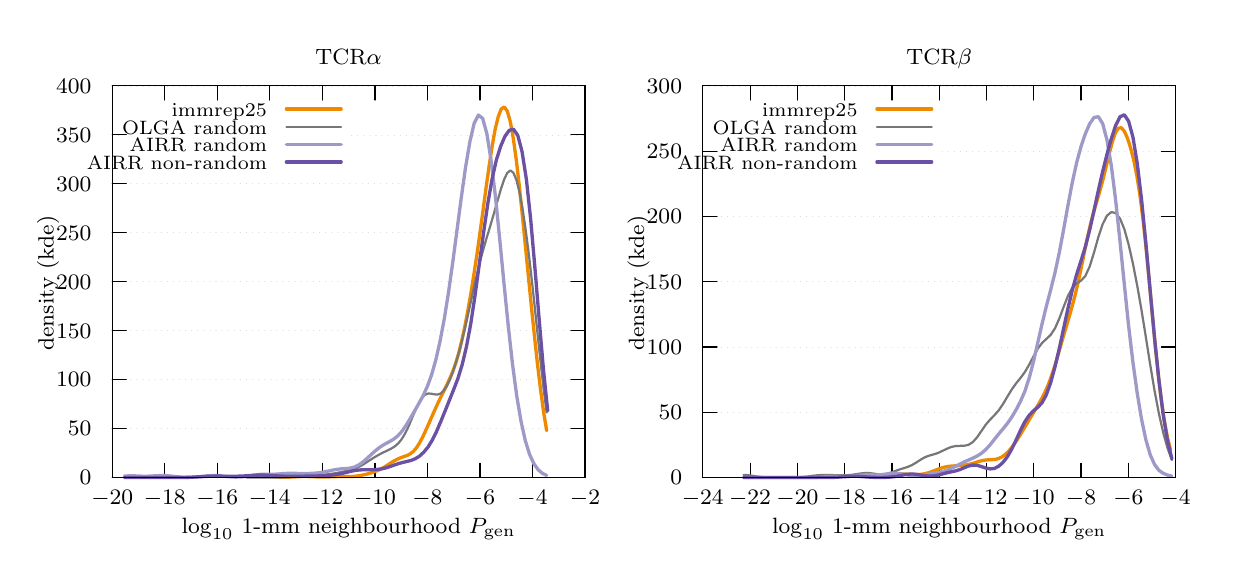
\begin{tikzpicture}[gnuplot]
%% generated with GNUPLOT 6.0p4 (Lua 5.5; terminal rev. Jun 2020, script rev. 120)
%% Sun Jul  5 05:56:43 2026
\tikzset{every node/.append style={font={\fontsize{8.0pt}{9.6pt}\selectfont}}}
\path (0.000,0.000) rectangle (15.000,6.500);
\gpcolor{rgb color={0.867,0.867,0.867}}
\gpsetlinetype{gp lt axes}
\gpsetdashtype{gp dt axes}
\gpsetlinewidth{0.50}
\draw[gp path] (1.054,0.787)--(7.058,0.787);
\gpcolor{color=gp lt color border}
\gpsetlinetype{gp lt border}
\gpsetdashtype{gp dt solid}
\gpsetlinewidth{1.00}
\draw[gp path] (1.054,0.787)--(1.234,0.787);
\draw[gp path] (7.058,0.787)--(6.878,0.787);
\node[gp node right,font={\fontsize{8.0pt}{9.6pt}\selectfont}] at (0.907,0.787) {$0$};
\gpcolor{rgb color={0.867,0.867,0.867}}
\gpsetlinetype{gp lt axes}
\gpsetdashtype{gp dt axes}
\gpsetlinewidth{0.50}
\draw[gp path] (1.054,1.409)--(7.058,1.409);
\gpcolor{color=gp lt color border}
\gpsetlinetype{gp lt border}
\gpsetdashtype{gp dt solid}
\gpsetlinewidth{1.00}
\draw[gp path] (1.054,1.409)--(1.234,1.409);
\draw[gp path] (7.058,1.409)--(6.878,1.409);
\node[gp node right,font={\fontsize{8.0pt}{9.6pt}\selectfont}] at (0.907,1.409) {$50$};
\gpcolor{rgb color={0.867,0.867,0.867}}
\gpsetlinetype{gp lt axes}
\gpsetdashtype{gp dt axes}
\gpsetlinewidth{0.50}
\draw[gp path] (1.054,2.031)--(7.058,2.031);
\gpcolor{color=gp lt color border}
\gpsetlinetype{gp lt border}
\gpsetdashtype{gp dt solid}
\gpsetlinewidth{1.00}
\draw[gp path] (1.054,2.031)--(1.234,2.031);
\draw[gp path] (7.058,2.031)--(6.878,2.031);
\node[gp node right,font={\fontsize{8.0pt}{9.6pt}\selectfont}] at (0.907,2.031) {$100$};
\gpcolor{rgb color={0.867,0.867,0.867}}
\gpsetlinetype{gp lt axes}
\gpsetdashtype{gp dt axes}
\gpsetlinewidth{0.50}
\draw[gp path] (1.054,2.652)--(7.058,2.652);
\gpcolor{color=gp lt color border}
\gpsetlinetype{gp lt border}
\gpsetdashtype{gp dt solid}
\gpsetlinewidth{1.00}
\draw[gp path] (1.054,2.652)--(1.234,2.652);
\draw[gp path] (7.058,2.652)--(6.878,2.652);
\node[gp node right,font={\fontsize{8.0pt}{9.6pt}\selectfont}] at (0.907,2.652) {$150$};
\gpcolor{rgb color={0.867,0.867,0.867}}
\gpsetlinetype{gp lt axes}
\gpsetdashtype{gp dt axes}
\gpsetlinewidth{0.50}
\draw[gp path] (1.054,3.274)--(7.058,3.274);
\gpcolor{color=gp lt color border}
\gpsetlinetype{gp lt border}
\gpsetdashtype{gp dt solid}
\gpsetlinewidth{1.00}
\draw[gp path] (1.054,3.274)--(1.234,3.274);
\draw[gp path] (7.058,3.274)--(6.878,3.274);
\node[gp node right,font={\fontsize{8.0pt}{9.6pt}\selectfont}] at (0.907,3.274) {$200$};
\gpcolor{rgb color={0.867,0.867,0.867}}
\gpsetlinetype{gp lt axes}
\gpsetdashtype{gp dt axes}
\gpsetlinewidth{0.50}
\draw[gp path] (1.054,3.896)--(7.058,3.896);
\gpcolor{color=gp lt color border}
\gpsetlinetype{gp lt border}
\gpsetdashtype{gp dt solid}
\gpsetlinewidth{1.00}
\draw[gp path] (1.054,3.896)--(1.234,3.896);
\draw[gp path] (7.058,3.896)--(6.878,3.896);
\node[gp node right,font={\fontsize{8.0pt}{9.6pt}\selectfont}] at (0.907,3.896) {$250$};
\gpcolor{rgb color={0.867,0.867,0.867}}
\gpsetlinetype{gp lt axes}
\gpsetdashtype{gp dt axes}
\gpsetlinewidth{0.50}
\draw[gp path] (1.054,4.518)--(7.058,4.518);
\gpcolor{color=gp lt color border}
\gpsetlinetype{gp lt border}
\gpsetdashtype{gp dt solid}
\gpsetlinewidth{1.00}
\draw[gp path] (1.054,4.518)--(1.234,4.518);
\draw[gp path] (7.058,4.518)--(6.878,4.518);
\node[gp node right,font={\fontsize{8.0pt}{9.6pt}\selectfont}] at (0.907,4.518) {$300$};
\gpcolor{rgb color={0.867,0.867,0.867}}
\gpsetlinetype{gp lt axes}
\gpsetdashtype{gp dt axes}
\gpsetlinewidth{0.50}
\draw[gp path] (1.054,5.139)--(1.201,5.139);
\draw[gp path] (4.090,5.139)--(7.058,5.139);
\gpcolor{color=gp lt color border}
\gpsetlinetype{gp lt border}
\gpsetdashtype{gp dt solid}
\gpsetlinewidth{1.00}
\draw[gp path] (1.054,5.139)--(1.234,5.139);
\draw[gp path] (7.058,5.139)--(6.878,5.139);
\node[gp node right,font={\fontsize{8.0pt}{9.6pt}\selectfont}] at (0.907,5.139) {$350$};
\gpcolor{rgb color={0.867,0.867,0.867}}
\gpsetlinetype{gp lt axes}
\gpsetdashtype{gp dt axes}
\gpsetlinewidth{0.50}
\draw[gp path] (1.054,5.761)--(7.058,5.761);
\gpcolor{color=gp lt color border}
\gpsetlinetype{gp lt border}
\gpsetdashtype{gp dt solid}
\gpsetlinewidth{1.00}
\draw[gp path] (1.054,5.761)--(1.234,5.761);
\draw[gp path] (7.058,5.761)--(6.878,5.761);
\node[gp node right,font={\fontsize{8.0pt}{9.6pt}\selectfont}] at (0.907,5.761) {$400$};
\draw[gp path] (1.054,0.787)--(1.054,0.967);
\draw[gp path] (1.054,5.761)--(1.054,5.581);
\node[gp node center,font={\fontsize{8.0pt}{9.6pt}\selectfont}] at (1.054,0.541) {$-20$};
\draw[gp path] (1.721,0.787)--(1.721,0.967);
\draw[gp path] (1.721,5.761)--(1.721,5.581);
\node[gp node center,font={\fontsize{8.0pt}{9.6pt}\selectfont}] at (1.721,0.541) {$-18$};
\draw[gp path] (2.388,0.787)--(2.388,0.967);
\draw[gp path] (2.388,5.761)--(2.388,5.581);
\node[gp node center,font={\fontsize{8.0pt}{9.6pt}\selectfont}] at (2.388,0.541) {$-16$};
\draw[gp path] (3.055,0.787)--(3.055,0.967);
\draw[gp path] (3.055,5.761)--(3.055,5.581);
\node[gp node center,font={\fontsize{8.0pt}{9.6pt}\selectfont}] at (3.055,0.541) {$-14$};
\draw[gp path] (3.722,0.787)--(3.722,0.967);
\draw[gp path] (3.722,5.761)--(3.722,5.581);
\node[gp node center,font={\fontsize{8.0pt}{9.6pt}\selectfont}] at (3.722,0.541) {$-12$};
\draw[gp path] (4.390,0.787)--(4.390,0.967);
\draw[gp path] (4.390,5.761)--(4.390,5.581);
\node[gp node center,font={\fontsize{8.0pt}{9.6pt}\selectfont}] at (4.390,0.541) {$-10$};
\draw[gp path] (5.057,0.787)--(5.057,0.967);
\draw[gp path] (5.057,5.761)--(5.057,5.581);
\node[gp node center,font={\fontsize{8.0pt}{9.6pt}\selectfont}] at (5.057,0.541) {$-8$};
\draw[gp path] (5.724,0.787)--(5.724,0.967);
\draw[gp path] (5.724,5.761)--(5.724,5.581);
\node[gp node center,font={\fontsize{8.0pt}{9.6pt}\selectfont}] at (5.724,0.541) {$-6$};
\draw[gp path] (6.391,0.787)--(6.391,0.967);
\draw[gp path] (6.391,5.761)--(6.391,5.581);
\node[gp node center,font={\fontsize{8.0pt}{9.6pt}\selectfont}] at (6.391,0.541) {$-4$};
\draw[gp path] (7.058,0.787)--(7.058,0.967);
\draw[gp path] (7.058,5.761)--(7.058,5.581);
\node[gp node center,font={\fontsize{8.0pt}{9.6pt}\selectfont}] at (7.058,0.541) {$-2$};
\draw[gp path] (1.054,5.761)--(1.054,0.787)--(7.058,0.787)--(7.058,5.761)--cycle;
\node[gp node right,font={\fontsize{7.0pt}{8.4pt}\selectfont}] at (3.136,5.468) {immrep25};
\gpcolor{rgb color={0.937,0.541,0.000}}
\gpsetlinewidth{3.00}
\draw[gp path] (3.265,5.468)--(3.961,5.468);
\draw[gp path] (2.761,0.802)--(2.800,0.803)--(2.838,0.804)--(2.876,0.804)--(2.915,0.804)%
  --(2.953,0.803)--(2.992,0.802)--(3.030,0.800)--(3.069,0.798)--(3.107,0.796)--(3.146,0.794)%
  --(3.184,0.792)--(3.223,0.791)--(3.261,0.791)--(3.300,0.792)--(3.338,0.793)--(3.377,0.795)%
  --(3.415,0.797)--(3.454,0.799)--(3.492,0.799)--(3.531,0.799)--(3.569,0.798)--(3.608,0.797)%
  --(3.646,0.795)--(3.685,0.794)--(3.723,0.793)--(3.762,0.793)--(3.800,0.795)--(3.838,0.796)%
  --(3.877,0.798)--(3.915,0.799)--(3.954,0.800)--(3.992,0.800)--(4.031,0.800)--(4.069,0.800)%
  --(4.108,0.801)--(4.146,0.804)--(4.185,0.809)--(4.223,0.816)--(4.262,0.824)--(4.300,0.834)%
  --(4.339,0.845)--(4.377,0.858)--(4.416,0.873)--(4.454,0.890)--(4.493,0.910)--(4.531,0.933)%
  --(4.570,0.958)--(4.608,0.983)--(4.647,1.006)--(4.685,1.025)--(4.724,1.041)--(4.762,1.054)%
  --(4.801,1.068)--(4.839,1.088)--(4.877,1.118)--(4.916,1.163)--(4.954,1.222)--(4.993,1.294)%
  --(5.031,1.376)--(5.070,1.462)--(5.108,1.550)--(5.147,1.638)--(5.185,1.722)--(5.224,1.803)%
  --(5.262,1.881)--(5.301,1.959)--(5.339,2.040)--(5.378,2.132)--(5.416,2.240)--(5.455,2.371)%
  --(5.493,2.527)--(5.532,2.707)--(5.570,2.909)--(5.609,3.130)--(5.647,3.369)--(5.686,3.625)%
  --(5.724,3.897)--(5.763,4.181)--(5.801,4.466)--(5.840,4.742)--(5.878,4.993)--(5.916,5.206)%
  --(5.955,5.367)--(5.993,5.466)--(6.032,5.493)--(6.070,5.441)--(6.109,5.307)--(6.147,5.094)%
  --(6.186,4.814)--(6.224,4.480)--(6.263,4.111)--(6.301,3.724)--(6.340,3.331)--(6.378,2.943)%
  --(6.417,2.570)--(6.455,2.218)--(6.494,1.898)--(6.532,1.618)--(6.571,1.382);
\gpcolor{color=gp lt color border}
\node[gp node right,font={\fontsize{7.0pt}{8.4pt}\selectfont}] at (3.136,5.243) {OLGA random};
\gpcolor{rgb color={0.467,0.467,0.467}}
\gpsetlinewidth{2.00}
\draw[gp path] (3.265,5.243)--(3.961,5.243);
\draw[gp path] (2.761,0.787)--(2.800,0.787)--(2.838,0.787)--(2.876,0.787)--(2.915,0.787)%
  --(2.953,0.787)--(2.992,0.787)--(3.030,0.787)--(3.069,0.787)--(3.107,0.787)--(3.146,0.788)%
  --(3.184,0.788)--(3.223,0.789)--(3.261,0.791)--(3.300,0.793)--(3.338,0.796)--(3.377,0.800)%
  --(3.415,0.804)--(3.454,0.808)--(3.492,0.811)--(3.531,0.814)--(3.569,0.816)--(3.608,0.817)%
  --(3.646,0.818)--(3.685,0.820)--(3.723,0.822)--(3.762,0.825)--(3.800,0.829)--(3.838,0.834)%
  --(3.877,0.840)--(3.915,0.847)--(3.954,0.855)--(3.992,0.863)--(4.031,0.871)--(4.069,0.880)%
  --(4.108,0.891)--(4.146,0.905)--(4.185,0.922)--(4.223,0.942)--(4.262,0.966)--(4.300,0.991)%
  --(4.339,1.016)--(4.377,1.040)--(4.416,1.063)--(4.454,1.084)--(4.493,1.104)--(4.531,1.122)%
  --(4.570,1.141)--(4.608,1.161)--(4.647,1.186)--(4.685,1.220)--(4.724,1.266)--(4.762,1.327)%
  --(4.801,1.401)--(4.839,1.488)--(4.877,1.580)--(4.916,1.669)--(4.954,1.747)--(4.993,1.805)%
  --(5.031,1.841)--(5.070,1.854)--(5.108,1.851)--(5.147,1.843)--(5.185,1.841)--(5.224,1.854)%
  --(5.262,1.889)--(5.301,1.946)--(5.339,2.025)--(5.378,2.124)--(5.416,2.239)--(5.455,2.370)%
  --(5.493,2.516)--(5.532,2.676)--(5.570,2.847)--(5.609,3.024)--(5.647,3.201)--(5.686,3.370)%
  --(5.724,3.528)--(5.763,3.673)--(5.801,3.806)--(5.840,3.934)--(5.878,4.062)--(5.916,4.194)%
  --(5.955,4.329)--(5.993,4.461)--(6.032,4.575)--(6.070,4.655)--(6.109,4.687)--(6.147,4.659)%
  --(6.186,4.569)--(6.224,4.417)--(6.263,4.210)--(6.301,3.955)--(6.340,3.659)--(6.378,3.330)%
  --(6.417,2.977)--(6.455,2.612)--(6.494,2.252)--(6.532,1.913)--(6.571,1.612);
\gpcolor{color=gp lt color border}
\node[gp node right,font={\fontsize{7.0pt}{8.4pt}\selectfont}] at (3.136,5.018) {AIRR random};
\gpcolor{rgb color={0.620,0.604,0.784}}
\gpsetlinewidth{3.00}
\draw[gp path] (3.265,5.018)--(3.961,5.018);
\draw[gp path] (1.208,0.806)--(1.262,0.808)--(1.316,0.808)--(1.370,0.807)--(1.424,0.804)%
  --(1.479,0.803)--(1.533,0.805)--(1.587,0.808)--(1.641,0.811)--(1.695,0.812)--(1.749,0.810)%
  --(1.804,0.805)--(1.858,0.799)--(1.912,0.794)--(1.966,0.790)--(2.020,0.789)--(2.074,0.790)%
  --(2.129,0.794)--(2.183,0.799)--(2.237,0.804)--(2.291,0.810)--(2.345,0.812)--(2.400,0.810)%
  --(2.454,0.805)--(2.508,0.799)--(2.562,0.795)--(2.616,0.792)--(2.670,0.793)--(2.725,0.798)%
  --(2.779,0.805)--(2.833,0.814)--(2.887,0.822)--(2.941,0.827)--(2.995,0.828)--(3.050,0.828)%
  --(3.104,0.828)--(3.158,0.831)--(3.212,0.836)--(3.266,0.839)--(3.320,0.841)--(3.375,0.840)%
  --(3.429,0.838)--(3.483,0.837)--(3.537,0.838)--(3.591,0.840)--(3.645,0.844)--(3.700,0.850)%
  --(3.754,0.860)--(3.808,0.871)--(3.862,0.883)--(3.916,0.892)--(3.970,0.898)--(4.025,0.901)%
  --(4.079,0.907)--(4.133,0.921)--(4.187,0.948)--(4.241,0.987)--(4.295,1.035)--(4.350,1.086)%
  --(4.404,1.134)--(4.458,1.176)--(4.512,1.209)--(4.566,1.238)--(4.621,1.270)--(4.675,1.311)%
  --(4.729,1.369)--(4.783,1.446)--(4.837,1.535)--(4.891,1.629)--(4.946,1.724)--(5.000,1.823)%
  --(5.054,1.940)--(5.108,2.087)--(5.162,2.277)--(5.216,2.514)--(5.271,2.804)--(5.325,3.144)%
  --(5.379,3.527)--(5.433,3.936)--(5.487,4.346)--(5.541,4.729)--(5.596,5.054)--(5.650,5.285)%
  --(5.704,5.390)--(5.758,5.348)--(5.812,5.150)--(5.866,4.807)--(5.921,4.346)--(5.975,3.810)%
  --(6.029,3.250)--(6.083,2.711)--(6.137,2.228)--(6.191,1.820)--(6.246,1.497)--(6.300,1.253)%
  --(6.354,1.080)--(6.408,0.963)--(6.462,0.887)--(6.516,0.840)--(6.571,0.814);
\gpcolor{color=gp lt color border}
\node[gp node right,font={\fontsize{7.0pt}{8.4pt}\selectfont}] at (3.136,4.793) {AIRR non-random};
\gpcolor{rgb color={0.416,0.318,0.639}}
\draw[gp path] (3.265,4.793)--(3.961,4.793);
\draw[gp path] (1.208,0.787)--(1.262,0.787)--(1.316,0.787)--(1.371,0.787)--(1.425,0.787)%
  --(1.479,0.787)--(1.534,0.787)--(1.588,0.787)--(1.642,0.787)--(1.697,0.787)--(1.751,0.787)%
  --(1.805,0.787)--(1.859,0.787)--(1.914,0.787)--(1.968,0.788)--(2.022,0.789)--(2.077,0.792)%
  --(2.131,0.795)--(2.185,0.798)--(2.240,0.801)--(2.294,0.803)--(2.348,0.804)--(2.403,0.805)%
  --(2.457,0.804)--(2.511,0.804)--(2.565,0.803)--(2.620,0.803)--(2.674,0.805)--(2.728,0.807)%
  --(2.783,0.811)--(2.837,0.814)--(2.891,0.817)--(2.946,0.818)--(3.000,0.817)--(3.054,0.814)%
  --(3.109,0.810)--(3.163,0.807)--(3.217,0.805)--(3.271,0.803)--(3.326,0.802)--(3.380,0.802)%
  --(3.434,0.802)--(3.489,0.804)--(3.543,0.805)--(3.597,0.806)--(3.652,0.807)--(3.706,0.809)%
  --(3.760,0.811)--(3.815,0.815)--(3.869,0.821)--(3.923,0.829)--(3.977,0.840)--(4.032,0.853)%
  --(4.086,0.866)--(4.140,0.877)--(4.195,0.883)--(4.249,0.886)--(4.303,0.886)--(4.358,0.886)%
  --(4.412,0.889)--(4.466,0.895)--(4.520,0.907)--(4.575,0.924)--(4.629,0.943)--(4.683,0.962)%
  --(4.738,0.977)--(4.792,0.990)--(4.846,1.003)--(4.901,1.025)--(4.955,1.058)--(5.009,1.108)%
  --(5.064,1.174)--(5.118,1.262)--(5.172,1.371)--(5.226,1.498)--(5.281,1.633)--(5.335,1.768)%
  --(5.389,1.902)--(5.444,2.046)--(5.498,2.221)--(5.552,2.448)--(5.607,2.742)--(5.661,3.098)%
  --(5.715,3.496)--(5.770,3.899)--(5.824,4.269)--(5.878,4.580)--(5.932,4.820)--(5.987,4.995)%
  --(6.041,5.120)--(6.095,5.196)--(6.150,5.210)--(6.204,5.131)--(6.258,4.927)--(6.313,4.575)%
  --(6.367,4.074)--(6.421,3.457)--(6.476,2.790)--(6.530,2.158)--(6.584,1.634);
\gpcolor{color=gp lt color border}
\gpsetlinewidth{1.00}
\draw[gp path] (1.054,5.761)--(1.054,0.787)--(7.058,0.787)--(7.058,5.761)--cycle;
\node[gp node center,rotate=-270.0,font={\fontsize{8.0pt}{9.6pt}\selectfont}] at (0.232,3.274) {density (kde)};
\node[gp node center,font={\fontsize{8.0pt}{9.6pt}\selectfont}] at (4.056,0.172) {$\log_{10}$ 1-mm neighbourhood $P_\mathrm{gen}$};
\node[gp node center,font={\fontsize{8.0pt}{9.6pt}\selectfont}] at (4.056,6.130) {TCR$\alpha$};
%% coordinates of the plot area
\gpdefrectangularnode{gp plot 1}{\pgfpoint{1.054cm}{0.787cm}}{\pgfpoint{7.058cm}{5.761cm}}
\gpcolor{rgb color={0.867,0.867,0.867}}
\gpsetlinetype{gp lt axes}
\gpsetdashtype{gp dt axes}
\gpsetlinewidth{0.50}
\draw[gp path] (8.554,0.787)--(14.558,0.787);
\gpcolor{color=gp lt color border}
\gpsetlinetype{gp lt border}
\gpsetdashtype{gp dt solid}
\gpsetlinewidth{1.00}
\draw[gp path] (8.554,0.787)--(8.734,0.787);
\draw[gp path] (14.558,0.787)--(14.378,0.787);
\node[gp node right,font={\fontsize{8.0pt}{9.6pt}\selectfont}] at (8.407,0.787) {$0$};
\gpcolor{rgb color={0.867,0.867,0.867}}
\gpsetlinetype{gp lt axes}
\gpsetdashtype{gp dt axes}
\gpsetlinewidth{0.50}
\draw[gp path] (8.554,1.616)--(14.558,1.616);
\gpcolor{color=gp lt color border}
\gpsetlinetype{gp lt border}
\gpsetdashtype{gp dt solid}
\gpsetlinewidth{1.00}
\draw[gp path] (8.554,1.616)--(8.734,1.616);
\draw[gp path] (14.558,1.616)--(14.378,1.616);
\node[gp node right,font={\fontsize{8.0pt}{9.6pt}\selectfont}] at (8.407,1.616) {$50$};
\gpcolor{rgb color={0.867,0.867,0.867}}
\gpsetlinetype{gp lt axes}
\gpsetdashtype{gp dt axes}
\gpsetlinewidth{0.50}
\draw[gp path] (8.554,2.445)--(14.558,2.445);
\gpcolor{color=gp lt color border}
\gpsetlinetype{gp lt border}
\gpsetdashtype{gp dt solid}
\gpsetlinewidth{1.00}
\draw[gp path] (8.554,2.445)--(8.734,2.445);
\draw[gp path] (14.558,2.445)--(14.378,2.445);
\node[gp node right,font={\fontsize{8.0pt}{9.6pt}\selectfont}] at (8.407,2.445) {$100$};
\gpcolor{rgb color={0.867,0.867,0.867}}
\gpsetlinetype{gp lt axes}
\gpsetdashtype{gp dt axes}
\gpsetlinewidth{0.50}
\draw[gp path] (8.554,3.274)--(14.558,3.274);
\gpcolor{color=gp lt color border}
\gpsetlinetype{gp lt border}
\gpsetdashtype{gp dt solid}
\gpsetlinewidth{1.00}
\draw[gp path] (8.554,3.274)--(8.734,3.274);
\draw[gp path] (14.558,3.274)--(14.378,3.274);
\node[gp node right,font={\fontsize{8.0pt}{9.6pt}\selectfont}] at (8.407,3.274) {$150$};
\gpcolor{rgb color={0.867,0.867,0.867}}
\gpsetlinetype{gp lt axes}
\gpsetdashtype{gp dt axes}
\gpsetlinewidth{0.50}
\draw[gp path] (8.554,4.103)--(14.558,4.103);
\gpcolor{color=gp lt color border}
\gpsetlinetype{gp lt border}
\gpsetdashtype{gp dt solid}
\gpsetlinewidth{1.00}
\draw[gp path] (8.554,4.103)--(8.734,4.103);
\draw[gp path] (14.558,4.103)--(14.378,4.103);
\node[gp node right,font={\fontsize{8.0pt}{9.6pt}\selectfont}] at (8.407,4.103) {$200$};
\gpcolor{rgb color={0.867,0.867,0.867}}
\gpsetlinetype{gp lt axes}
\gpsetdashtype{gp dt axes}
\gpsetlinewidth{0.50}
\draw[gp path] (8.554,4.932)--(8.701,4.932);
\draw[gp path] (11.590,4.932)--(14.558,4.932);
\gpcolor{color=gp lt color border}
\gpsetlinetype{gp lt border}
\gpsetdashtype{gp dt solid}
\gpsetlinewidth{1.00}
\draw[gp path] (8.554,4.932)--(8.734,4.932);
\draw[gp path] (14.558,4.932)--(14.378,4.932);
\node[gp node right,font={\fontsize{8.0pt}{9.6pt}\selectfont}] at (8.407,4.932) {$250$};
\gpcolor{rgb color={0.867,0.867,0.867}}
\gpsetlinetype{gp lt axes}
\gpsetdashtype{gp dt axes}
\gpsetlinewidth{0.50}
\draw[gp path] (8.554,5.761)--(14.558,5.761);
\gpcolor{color=gp lt color border}
\gpsetlinetype{gp lt border}
\gpsetdashtype{gp dt solid}
\gpsetlinewidth{1.00}
\draw[gp path] (8.554,5.761)--(8.734,5.761);
\draw[gp path] (14.558,5.761)--(14.378,5.761);
\node[gp node right,font={\fontsize{8.0pt}{9.6pt}\selectfont}] at (8.407,5.761) {$300$};
\draw[gp path] (8.554,0.787)--(8.554,0.967);
\draw[gp path] (8.554,5.761)--(8.554,5.581);
\node[gp node center,font={\fontsize{8.0pt}{9.6pt}\selectfont}] at (8.554,0.541) {$-24$};
\draw[gp path] (9.154,0.787)--(9.154,0.967);
\draw[gp path] (9.154,5.761)--(9.154,5.581);
\node[gp node center,font={\fontsize{8.0pt}{9.6pt}\selectfont}] at (9.154,0.541) {$-22$};
\draw[gp path] (9.755,0.787)--(9.755,0.967);
\draw[gp path] (9.755,5.761)--(9.755,5.581);
\node[gp node center,font={\fontsize{8.0pt}{9.6pt}\selectfont}] at (9.755,0.541) {$-20$};
\draw[gp path] (10.355,0.787)--(10.355,0.967);
\draw[gp path] (10.355,5.761)--(10.355,5.581);
\node[gp node center,font={\fontsize{8.0pt}{9.6pt}\selectfont}] at (10.355,0.541) {$-18$};
\draw[gp path] (10.956,0.787)--(10.956,0.967);
\draw[gp path] (10.956,5.761)--(10.956,5.581);
\node[gp node center,font={\fontsize{8.0pt}{9.6pt}\selectfont}] at (10.956,0.541) {$-16$};
\draw[gp path] (11.556,0.787)--(11.556,0.967);
\draw[gp path] (11.556,5.761)--(11.556,5.581);
\node[gp node center,font={\fontsize{8.0pt}{9.6pt}\selectfont}] at (11.556,0.541) {$-14$};
\draw[gp path] (12.156,0.787)--(12.156,0.967);
\draw[gp path] (12.156,5.761)--(12.156,5.581);
\node[gp node center,font={\fontsize{8.0pt}{9.6pt}\selectfont}] at (12.156,0.541) {$-12$};
\draw[gp path] (12.757,0.787)--(12.757,0.967);
\draw[gp path] (12.757,5.761)--(12.757,5.581);
\node[gp node center,font={\fontsize{8.0pt}{9.6pt}\selectfont}] at (12.757,0.541) {$-10$};
\draw[gp path] (13.357,0.787)--(13.357,0.967);
\draw[gp path] (13.357,5.761)--(13.357,5.581);
\node[gp node center,font={\fontsize{8.0pt}{9.6pt}\selectfont}] at (13.357,0.541) {$-8$};
\draw[gp path] (13.958,0.787)--(13.958,0.967);
\draw[gp path] (13.958,5.761)--(13.958,5.581);
\node[gp node center,font={\fontsize{8.0pt}{9.6pt}\selectfont}] at (13.958,0.541) {$-6$};
\draw[gp path] (14.558,0.787)--(14.558,0.967);
\draw[gp path] (14.558,5.761)--(14.558,5.581);
\node[gp node center,font={\fontsize{8.0pt}{9.6pt}\selectfont}] at (14.558,0.541) {$-4$};
\draw[gp path] (8.554,5.761)--(8.554,0.787)--(14.558,0.787)--(14.558,5.761)--cycle;
\node[gp node right,font={\fontsize{7.0pt}{8.4pt}\selectfont}] at (10.636,5.468) {immrep25};
\gpcolor{rgb color={0.937,0.541,0.000}}
\gpsetlinewidth{3.00}
\draw[gp path] (10.765,5.468)--(11.461,5.468);
\draw[gp path] (10.634,0.804)--(10.673,0.803)--(10.712,0.801)--(10.751,0.799)--(10.790,0.797)%
  --(10.829,0.797)--(10.868,0.800)--(10.907,0.805)--(10.946,0.811)--(10.985,0.819)--(11.024,0.825)%
  --(11.063,0.830)--(11.102,0.831)--(11.141,0.830)--(11.180,0.828)--(11.219,0.825)--(11.258,0.824)%
  --(11.297,0.825)--(11.336,0.829)--(11.375,0.836)--(11.414,0.846)--(11.453,0.859)--(11.492,0.874)%
  --(11.531,0.889)--(11.570,0.903)--(11.609,0.915)--(11.648,0.924)--(11.687,0.930)--(11.726,0.933)%
  --(11.765,0.936)--(11.804,0.938)--(11.843,0.941)--(11.882,0.945)--(11.921,0.951)--(11.960,0.960)%
  --(11.999,0.971)--(12.038,0.984)--(12.077,0.996)--(12.116,1.005)--(12.155,1.010)--(12.194,1.012)%
  --(12.233,1.014)--(12.272,1.018)--(12.311,1.029)--(12.350,1.047)--(12.389,1.075)--(12.428,1.111)%
  --(12.467,1.156)--(12.506,1.208)--(12.545,1.266)--(12.584,1.328)--(12.623,1.393)--(12.662,1.458)%
  --(12.701,1.524)--(12.740,1.589)--(12.779,1.654)--(12.818,1.719)--(12.857,1.788)--(12.896,1.864)%
  --(12.935,1.951)--(12.974,2.053)--(13.013,2.169)--(13.052,2.298)--(13.091,2.434)--(13.130,2.570)%
  --(13.169,2.702)--(13.208,2.833)--(13.246,2.968)--(13.285,3.116)--(13.324,3.283)--(13.363,3.467)%
  --(13.402,3.660)--(13.441,3.846)--(13.480,4.015)--(13.519,4.163)--(13.558,4.296)--(13.597,4.429)%
  --(13.636,4.572)--(13.675,4.730)--(13.714,4.893)--(13.753,5.044)--(13.792,5.160)--(13.831,5.224)%
  --(13.870,5.229)--(13.909,5.182)--(13.948,5.093)--(13.987,4.972)--(14.026,4.820)--(14.065,4.627)%
  --(14.104,4.382)--(14.143,4.076)--(14.182,3.713)--(14.221,3.308)--(14.260,2.885)--(14.299,2.472)%
  --(14.338,2.094)--(14.377,1.769)--(14.416,1.503)--(14.455,1.294)--(14.494,1.135);
\gpcolor{color=gp lt color border}
\node[gp node right,font={\fontsize{7.0pt}{8.4pt}\selectfont}] at (10.636,5.243) {OLGA random};
\gpcolor{rgb color={0.467,0.467,0.467}}
\gpsetlinewidth{2.00}
\draw[gp path] (10.765,5.243)--(11.461,5.243);
\draw[gp path] (9.071,0.820)--(9.126,0.817)--(9.181,0.809)--(9.236,0.801)--(9.291,0.794)%
  --(9.346,0.790)--(9.401,0.788)--(9.456,0.787)--(9.511,0.787)--(9.566,0.787)--(9.621,0.787)%
  --(9.676,0.787)--(9.731,0.788)--(9.786,0.791)--(9.841,0.795)--(9.895,0.801)--(9.950,0.809)%
  --(10.005,0.815)--(10.060,0.819)--(10.115,0.820)--(10.170,0.819)--(10.225,0.817)--(10.280,0.816)%
  --(10.335,0.815)--(10.390,0.817)--(10.445,0.821)--(10.500,0.829)--(10.555,0.838)--(10.610,0.844)%
  --(10.665,0.844)--(10.720,0.837)--(10.775,0.829)--(10.830,0.826)--(10.885,0.833)--(10.939,0.848)%
  --(10.994,0.868)--(11.049,0.888)--(11.104,0.905)--(11.159,0.923)--(11.214,0.947)--(11.269,0.980)%
  --(11.324,1.016)--(11.379,1.047)--(11.434,1.067)--(11.489,1.082)--(11.544,1.100)--(11.599,1.126)%
  --(11.654,1.153)--(11.709,1.175)--(11.764,1.186)--(11.819,1.189)--(11.874,1.190)--(11.928,1.202)%
  --(11.983,1.237)--(12.038,1.299)--(12.093,1.379)--(12.148,1.459)--(12.203,1.523)--(12.258,1.579)%
  --(12.313,1.642)--(12.368,1.723)--(12.423,1.816)--(12.478,1.906)--(12.533,1.983)--(12.588,2.051)%
  --(12.643,2.125)--(12.698,2.219)--(12.753,2.325)--(12.808,2.424)--(12.863,2.497)--(12.917,2.547)%
  --(12.972,2.599)--(13.027,2.683)--(13.082,2.808)--(13.137,2.956)--(13.192,3.096)--(13.247,3.196)%
  --(13.302,3.252)--(13.357,3.287)--(13.412,3.347)--(13.467,3.467)--(13.522,3.644)--(13.577,3.840)%
  --(13.632,4.005)--(13.687,4.113)--(13.742,4.158)--(13.797,4.146)--(13.852,4.076)--(13.907,3.942)%
  --(13.961,3.748)--(14.016,3.505)--(14.071,3.223)--(14.126,2.908)--(14.181,2.566)--(14.236,2.218)%
  --(14.291,1.889)--(14.346,1.599)--(14.401,1.356)--(14.456,1.159)--(14.511,1.010);
\gpcolor{color=gp lt color border}
\node[gp node right,font={\fontsize{7.0pt}{8.4pt}\selectfont}] at (10.636,5.018) {AIRR random};
\gpcolor{rgb color={0.620,0.604,0.784}}
\gpsetlinewidth{3.00}
\draw[gp path] (10.765,5.018)--(11.461,5.018);
\draw[gp path] (9.071,0.787)--(9.126,0.787)--(9.181,0.787)--(9.236,0.787)--(9.291,0.787)%
  --(9.346,0.787)--(9.401,0.787)--(9.456,0.787)--(9.511,0.787)--(9.566,0.787)--(9.621,0.787)%
  --(9.676,0.787)--(9.731,0.787)--(9.786,0.787)--(9.841,0.787)--(9.895,0.787)--(9.950,0.788)%
  --(10.005,0.789)--(10.060,0.792)--(10.115,0.796)--(10.170,0.800)--(10.225,0.803)--(10.280,0.804)%
  --(10.335,0.802)--(10.390,0.801)--(10.445,0.803)--(10.500,0.809)--(10.555,0.816)--(10.610,0.820)%
  --(10.665,0.821)--(10.720,0.820)--(10.775,0.820)--(10.830,0.824)--(10.885,0.831)--(10.939,0.838)%
  --(10.994,0.841)--(11.049,0.838)--(11.104,0.830)--(11.159,0.819)--(11.214,0.811)--(11.269,0.808)%
  --(11.324,0.812)--(11.379,0.820)--(11.434,0.831)--(11.489,0.841)--(11.544,0.851)--(11.599,0.863)%
  --(11.654,0.880)--(11.709,0.903)--(11.764,0.930)--(11.819,0.958)--(11.874,0.985)--(11.928,1.009)%
  --(11.983,1.033)--(12.038,1.060)--(12.093,1.095)--(12.148,1.143)--(12.203,1.203)--(12.258,1.273)%
  --(12.313,1.342)--(12.368,1.407)--(12.423,1.475)--(12.478,1.555)--(12.533,1.648)--(12.588,1.754)%
  --(12.643,1.881)--(12.698,2.047)--(12.753,2.258)--(12.808,2.500)--(12.863,2.742)--(12.917,2.963)%
  --(12.972,3.171)--(13.027,3.391)--(13.082,3.648)--(13.137,3.942)--(13.192,4.249)--(13.247,4.538)%
  --(13.302,4.788)--(13.357,4.991)--(13.412,5.153)--(13.467,5.279)--(13.522,5.359)--(13.577,5.370)%
  --(13.632,5.281)--(13.687,5.073)--(13.742,4.745)--(13.797,4.307)--(13.852,3.788)--(13.907,3.240)%
  --(13.961,2.716)--(14.016,2.252)--(14.071,1.856)--(14.126,1.526)--(14.181,1.265)--(14.236,1.075)%
  --(14.291,0.952)--(14.346,0.879)--(14.401,0.840)--(14.456,0.818)--(14.511,0.804);
\gpcolor{color=gp lt color border}
\node[gp node right,font={\fontsize{7.0pt}{8.4pt}\selectfont}] at (10.636,4.793) {AIRR non-random};
\gpcolor{rgb color={0.416,0.318,0.639}}
\draw[gp path] (10.765,4.793)--(11.461,4.793);
\draw[gp path] (9.071,0.787)--(9.126,0.787)--(9.181,0.787)--(9.236,0.787)--(9.291,0.787)%
  --(9.346,0.787)--(9.401,0.787)--(9.456,0.787)--(9.511,0.787)--(9.566,0.787)--(9.621,0.787)%
  --(9.676,0.787)--(9.731,0.787)--(9.786,0.787)--(9.841,0.787)--(9.895,0.787)--(9.950,0.787)%
  --(10.005,0.787)--(10.060,0.787)--(10.115,0.787)--(10.170,0.788)--(10.225,0.789)--(10.280,0.792)%
  --(10.335,0.796)--(10.390,0.800)--(10.445,0.803)--(10.500,0.803)--(10.555,0.800)--(10.610,0.796)%
  --(10.665,0.792)--(10.720,0.789)--(10.775,0.788)--(10.830,0.788)--(10.885,0.789)--(10.939,0.793)%
  --(10.994,0.799)--(11.049,0.809)--(11.104,0.820)--(11.159,0.829)--(11.214,0.832)--(11.269,0.827)%
  --(11.324,0.818)--(11.379,0.809)--(11.434,0.805)--(11.489,0.808)--(11.544,0.818)--(11.599,0.833)%
  --(11.654,0.847)--(11.709,0.859)--(11.764,0.871)--(11.819,0.888)--(11.874,0.911)--(11.928,0.933)%
  --(11.983,0.945)--(12.038,0.942)--(12.093,0.926)--(12.148,0.907)--(12.203,0.896)--(12.258,0.903)%
  --(12.313,0.931)--(12.368,0.981)--(12.423,1.053)--(12.478,1.150)--(12.533,1.265)--(12.588,1.385)%
  --(12.643,1.494)--(12.698,1.577)--(12.753,1.634)--(12.808,1.679)--(12.863,1.738)--(12.917,1.839)%
  --(12.972,1.993)--(13.027,2.194)--(13.082,2.430)--(13.137,2.685)--(13.192,2.939)--(13.247,3.171)%
  --(13.302,3.368)--(13.357,3.540)--(13.412,3.718)--(13.467,3.931)--(13.522,4.177)--(13.577,4.433)%
  --(13.632,4.674)--(13.687,4.893)--(13.742,5.092)--(13.797,5.258)--(13.852,5.368)--(13.907,5.393)%
  --(13.961,5.313)--(14.016,5.111)--(14.071,4.778)--(14.126,4.317)--(14.181,3.757)--(14.236,3.150)%
  --(14.291,2.556)--(14.346,2.024)--(14.401,1.583)--(14.456,1.249)--(14.511,1.023);
\gpcolor{color=gp lt color border}
\gpsetlinewidth{1.00}
\draw[gp path] (8.554,5.761)--(8.554,0.787)--(14.558,0.787)--(14.558,5.761)--cycle;
\node[gp node center,rotate=-270.0,font={\fontsize{8.0pt}{9.6pt}\selectfont}] at (7.732,3.274) {density (kde)};
\node[gp node center,font={\fontsize{8.0pt}{9.6pt}\selectfont}] at (11.556,0.172) {$\log_{10}$ 1-mm neighbourhood $P_\mathrm{gen}$};
\node[gp node center,font={\fontsize{8.0pt}{9.6pt}\selectfont}] at (11.556,6.130) {TCR$\beta$};
%% coordinates of the plot area
\gpdefrectangularnode{gp plot 2}{\pgfpoint{8.554cm}{0.787cm}}{\pgfpoint{14.558cm}{5.761cm}}
\end{tikzpicture}
%% gnuplot variables

\caption{1-mm neighbourhood $P_{\text{gen}}$ (kernel density) per chain. immrep25
overlaps its pgen-matched OLGA control (degree is controlled). The real AIRR repertoire
spans a decade of degree by sampling---lowest for unique clonotypes, highest for the
abundant top-frequency clones---yet both sit at homology S/N${\approx}1$
(Fig.~\ref{fig:hom}).}
\label{fig:pgen1mm}
\end{figure}

\section{Conclusion}\label{sec:conclusion}

Across both probes and both chains the calibration cohorts recover the expected
order, and the immrep25 positives fall at the bottom, just above the two OLGA random
floors and one to three orders of magnitude below every quality cohort
(Fig.~\ref{fig:ladder}). Their weak homology is contributed by public TCRs and
collapses to the floor when those are removed; their inter-chain pairing shows
essentially no coupling. We therefore find \emph{no meaningful epitope-specific
signal---in homology or chain pairing---among the immrep25 positives beyond noise and
publicity}, consistent with the benchmark's own finding that models do not exceed
random guessing on unseen peptides~\cite{Richardson2026}.

\begin{figure}[h]\centering
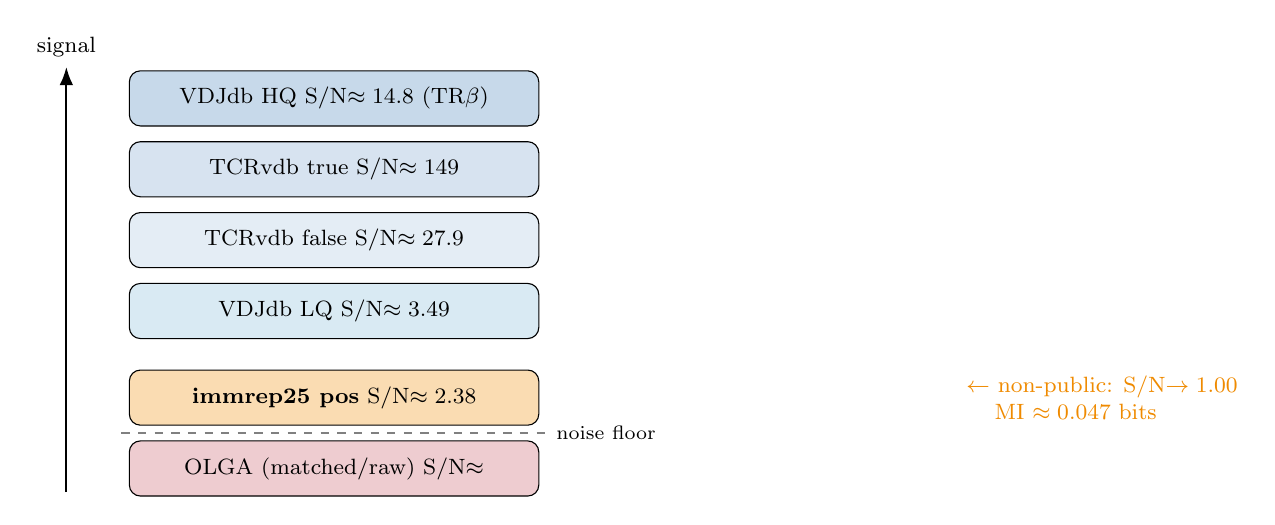
\begin{tikzpicture}[font=\footnotesize,>=Latex,
  rung/.style={draw,rounded corners,minimum width=52mm,minimum height=7mm,align=center}]
\definecolor{sig}{HTML}{2166ac}\definecolor{weak}{HTML}{67a9cf}
\definecolor{noise}{HTML}{b2182b}\definecolor{test}{HTML}{ef8a00}
\node[rung,fill=sig!25]  (a) at (0,5.0) {VDJdb HQ \hfill S/N$\approx\hqHomB$ (TR$\beta$)};
\node[rung,fill=sig!18]  (b) at (0,4.1) {TCRvdb true \hfill S/N$\approx\trueHomB$};
\node[rung,fill=sig!12]  (c) at (0,3.2) {TCRvdb false \hfill S/N$\approx\falseHomB$};
\node[rung,fill=weak!25] (d) at (0,2.3) {VDJdb LQ \hfill S/N$\approx\lqHomB$};
\node[rung,fill=test!30] (e) at (0,1.2) {\textbf{immrep25 pos} \hfill S/N$\approx\immHomB$};
\node[rung,fill=noise!22](f) at (0,0.3) {OLGA (matched/raw) \hfill S/N$\approx\olgaMHomB$};
\draw[->,thick] (-3.4,0.0) -- (-3.4,5.4) node[above,align=center]{signal};
\draw[dashed,gray] (-2.7,0.75) -- (2.7,0.75) node[right,black]{\scriptsize noise floor};
\node[test,right=1mm of e,xshift=52mm,align=left]
  {$\leftarrow$ non-public: S/N$\to\npHomB$\\\phantom{x}\ \ MI $\approx\immMi$ bits};
\end{tikzpicture}
\caption{Signal-to-noise ladder (TR$\beta$ homology, one-vs-many). The immrep25
positives sit one rung above the random floor; stripping public TCRs lowers them
onto it.}
\label{fig:ladder}
\end{figure}

\paragraph{Caveats.} TCRvdb true/false separate less than expected because
$p_{\text{adj}}$ scores differential enrichment in one screen rather than absence of
specificity, so ``false'' still contains epitope-associated TCRs; and TCRvdb and
VDJdb-HQ rest on only 2 and 5 epitopes respectively, so their absolute S/N is
uncertain (wide CIs). Neither affects immrep25, whose 20 epitopes place it just above
the OLGA floor on every probe. Reproduce with \texttt{bash scripts/fetch\_vdjdb.sh};
\texttt{python src/build\_olga.py}; \texttt{python run\_audit.py}; \texttt{make}.


\bibliographystyle{unsrt}
\bibliography{refs}
\end{document}
